\chapter{Estado da arte} \label{capitulo_2}

Esse capítulo detalha a modelagem geológica implícita com funções distância assinaladas, desde o cálculo das distâncias até a avaliação de incerteza dos modelos geológicos.

O fluxo de trabalho e os diferentes métodos disponíveis na literatura serão apresentados com exemplos práticos em um banco de dados tridimensional sintético que emula um depósito de cobre pórfiro. Pode ser encontrado na íntegra, com toda a memória de cálculo \href{https://drive.google.com/open?id=1JLRrOtOzDVCEpqnG8Ik95xws7Dw6MBvJ}{aqui}

\section{O banco de dados}

O banco de dados categóricos contém 72 furos totalizando 3349 amostras distribuídas entre 3 diferentes categorias conforme o histograma da \autoref{hist_geo}.

\begin{figure}[!htb]
	\caption{\label{hist_geo}Histograma do banco de dados.}
	\begin{center}
		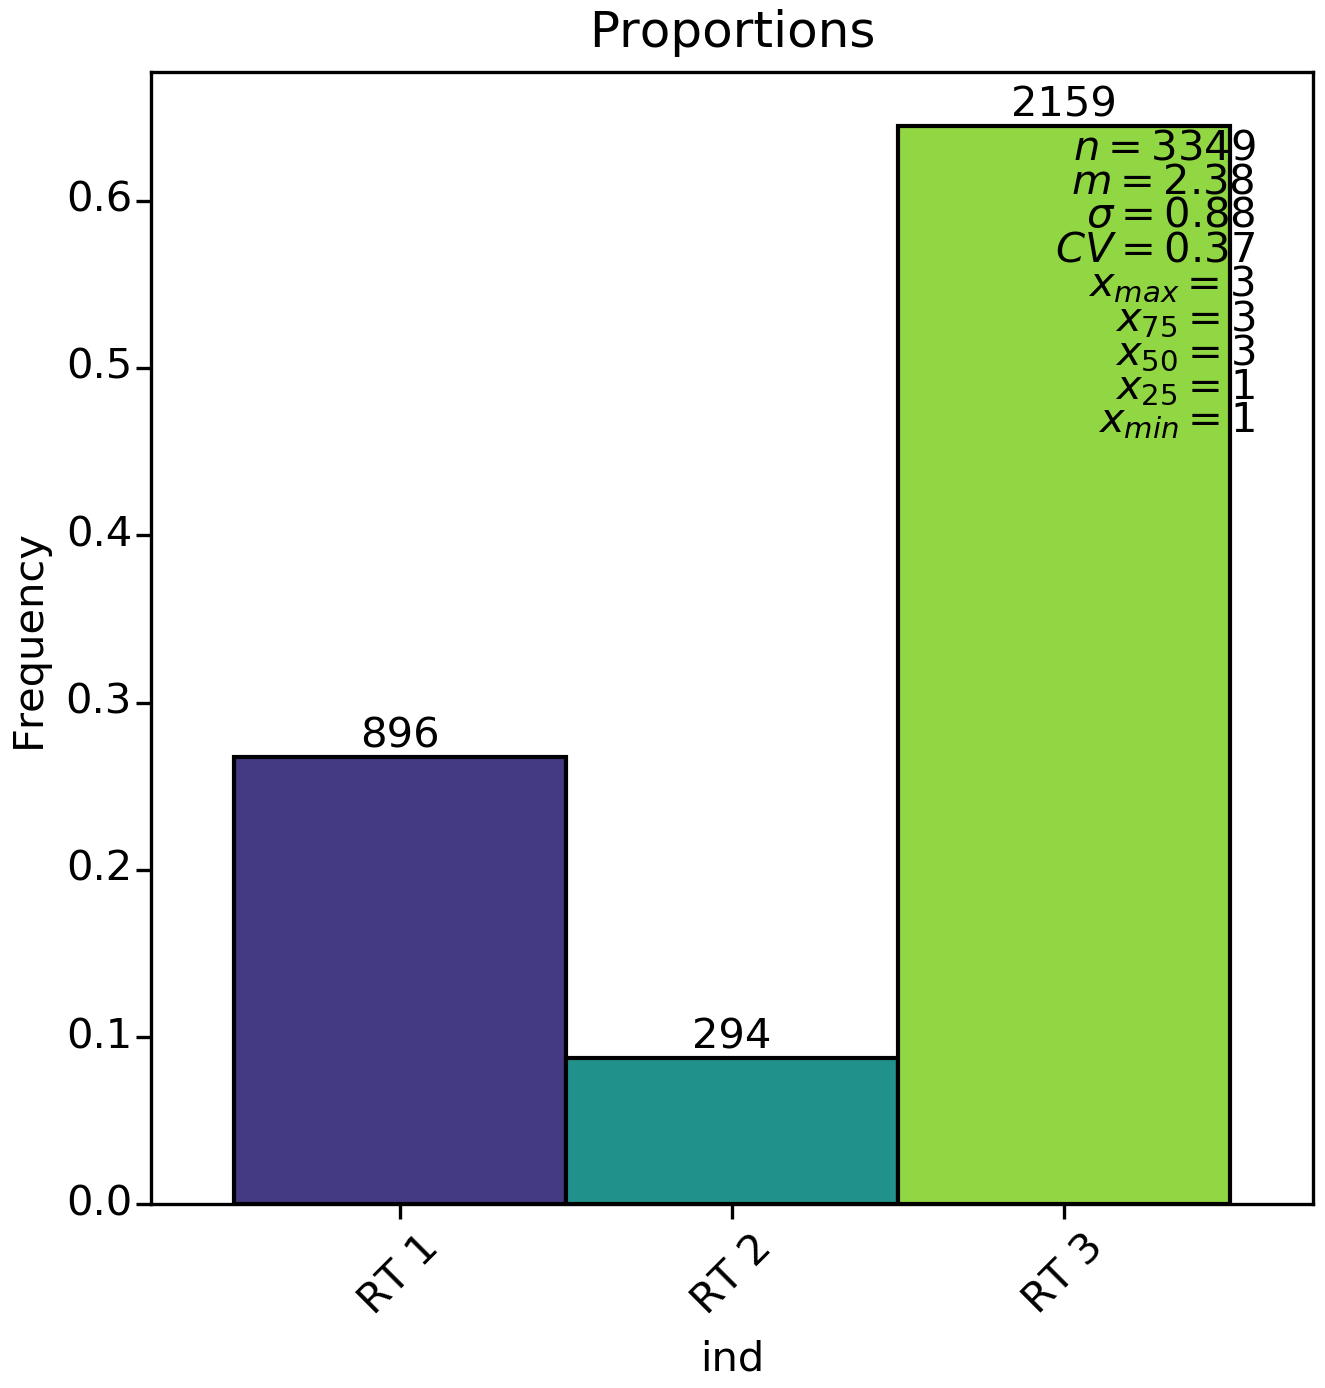
\includegraphics[width=0.5\textwidth]{capitulo_2/prop_hist.png}
	\end{center}
	%\legend{Modificado de \citeonline{martin2017implicitmodeling}}
\end{figure}

A \autoref{dataset} mostra a posição espacial das amostras do banco de dados tridimenional.

\begin{figure}[!htb]
	\caption{\label{dataset}Vista das amostras.}
	\begin{center}
		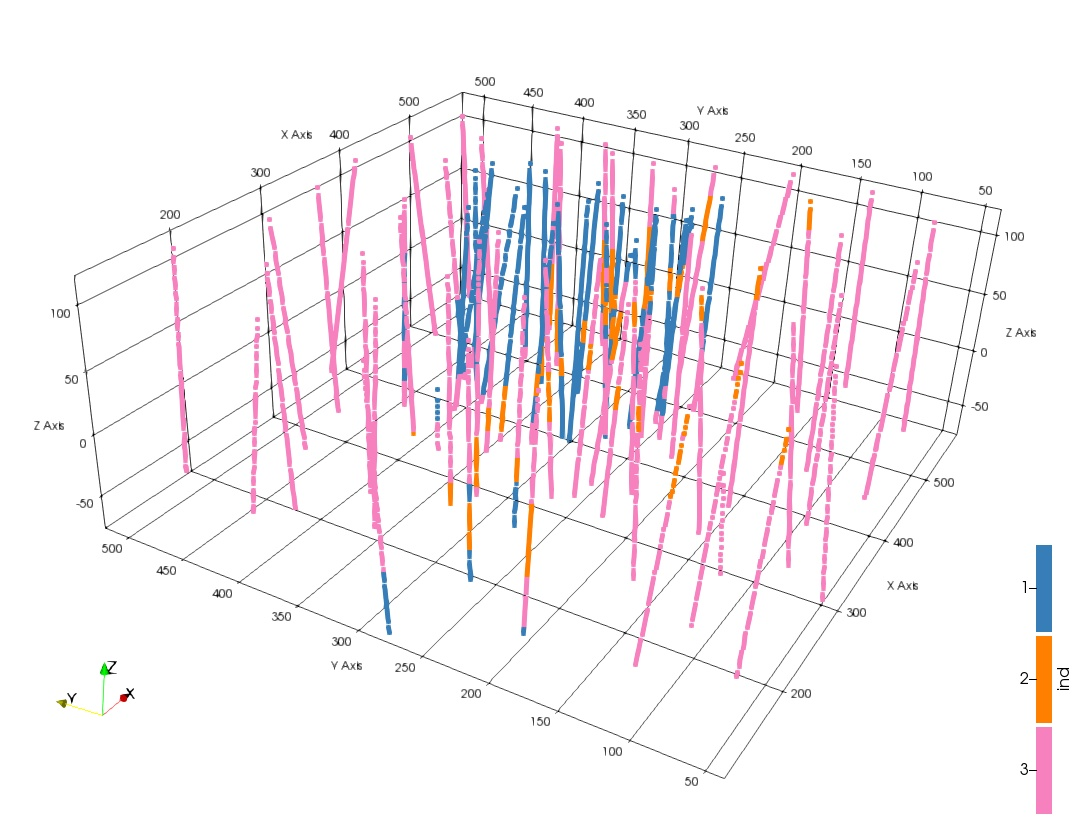
\includegraphics[width=0.8\textwidth]{capitulo_2/dados.jpeg}
	\end{center}
	%\legend{Modificado de \citeonline{martin2017implicitmodeling}}
\end{figure}

\section{A função distância assinalada}

A modelagem implícita é geralmente aplicada à variáveis categóricas que representam diferentes litologias do depósito mineral para definir a localização, extensão e geometria dos corpos minerais. A variável de indicadores deve ser codificada em uma função volumétrica e interpolada exaustivamente para todos os locais de interesse. A função distância assinalada \cite{osherlevelsetmethods}  é a função volume mais utilizada na modelagem implícita de variáveis categóricas.

\subsection{Calculando a função distância assinalada}

O primeiro passo no cálculo das distâncias assinaladas é transformar as amostras ${z(u_\alpha),\alpha=1,...,n}$ em indicadores binários de acordo com a \autoref{eq_ind}, especificando se a amostra pertence ou não ao domínio $k$ que está sendo modelado.

\begin{equation}
	i_k(u_\alpha)=\begin{cases}
	1,\:\textrm{se}\:z(u_\alpha)\:\textrm{se pertence ao domínio $k$}\\
	0,\:\textrm{se}\:z(u_\alpha)\:\textrm{caso contrário}\end{cases}
    \label{eq_ind}
\end{equation}

A \autoref{ind} mostra as amostras codificadas em indicadores para cada uma das três categorias do banco de dados.

\begin{figure}
    \caption{Amostras codificadas em indicadores para cada uma das três categorias do banco de dados.} \label{ind}
     \centering
     \subfloat[][Categoria 1]{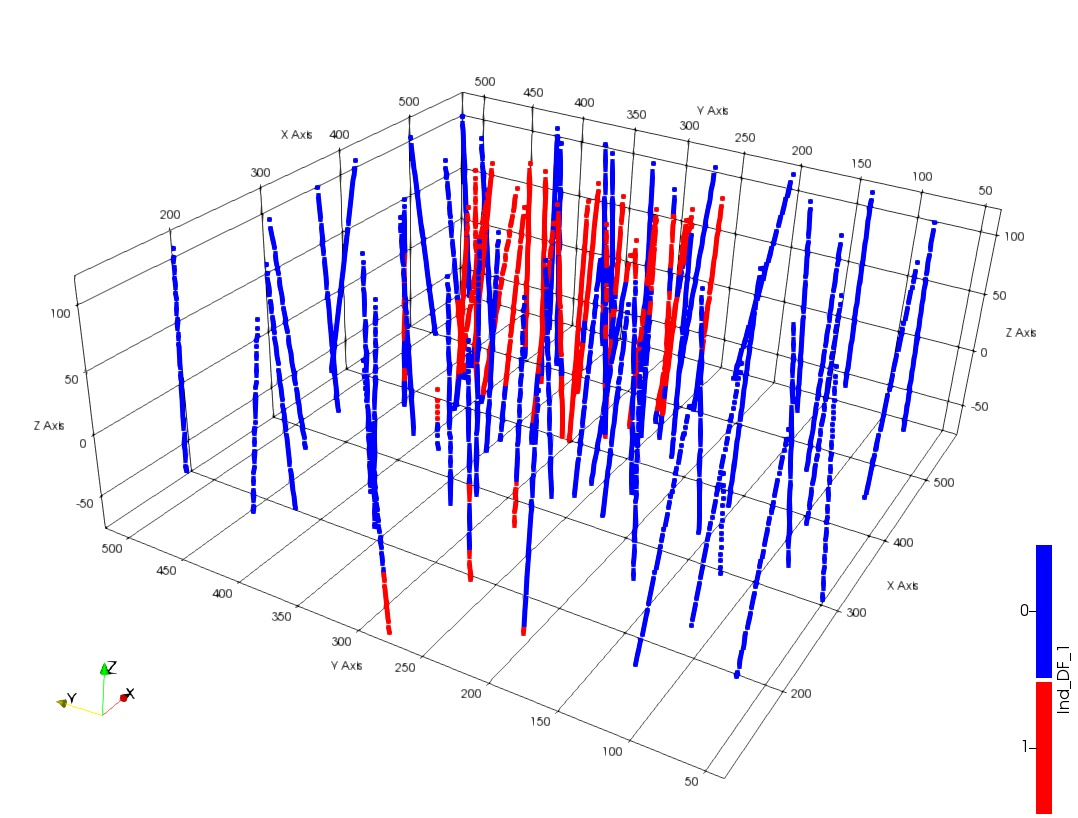
\includegraphics[width=.3\textwidth]{capitulo_2/inddf1.jpeg}\label{<figure1>}}
     \subfloat[][Categoria 2]{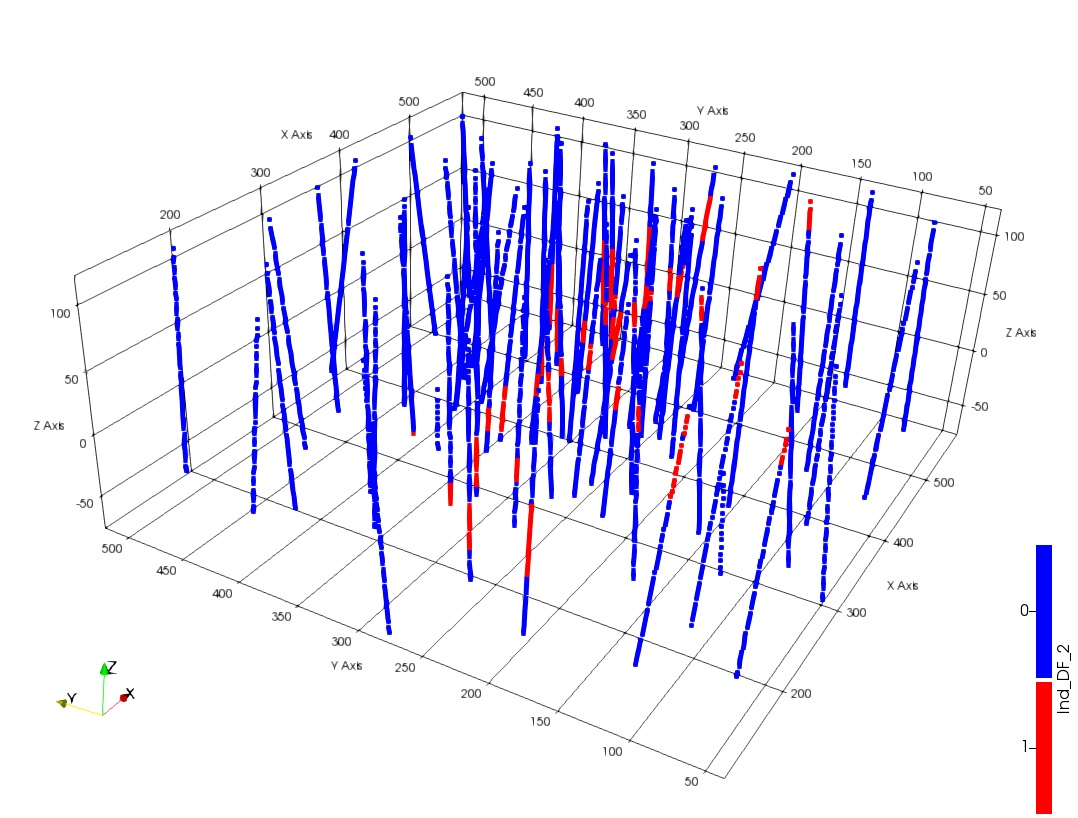
\includegraphics[width=.3\textwidth]{capitulo_2/inddf2.jpeg}\label{<figure2>}}
     \subfloat[][Categoria 3]{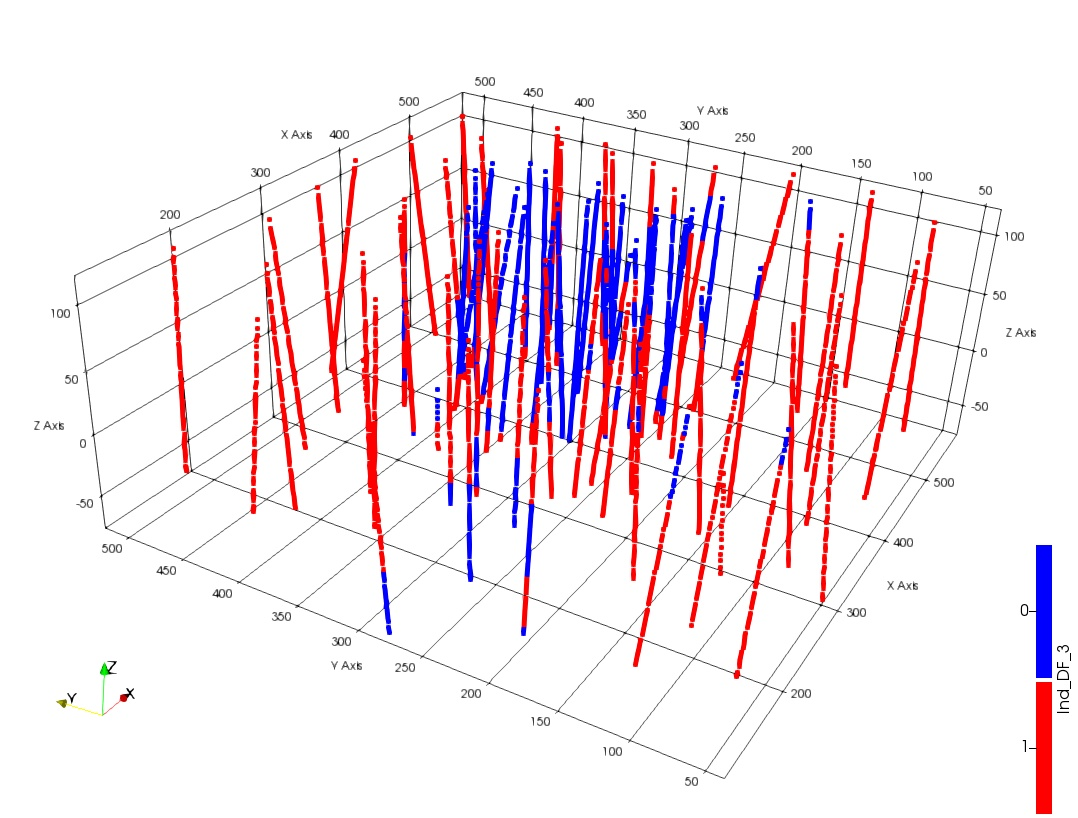
\includegraphics[width=.3\textwidth]{capitulo_2/inddf3.jpeg}\label{<figure2>}}
\end{figure}

O segundo passo é o cálculo das distâncias assinaladas. Para cada ponto amostral, a menor distância euclideana até um outro ponto amostral que pertence à um indicador oposto é computada, e esse valor atribuído àquele ponto, com o sinal negativo caso pertença ao domínio modelado e com o sinal positivo, caso contrário como ilustrado na \autoref{2d_ex}. 

\begin{figure}[!htb]
	\caption{\label{2d_ex}Ilustração esquemática mostrando o cálculo das distâncias assinaladas.}
	\begin{center}
		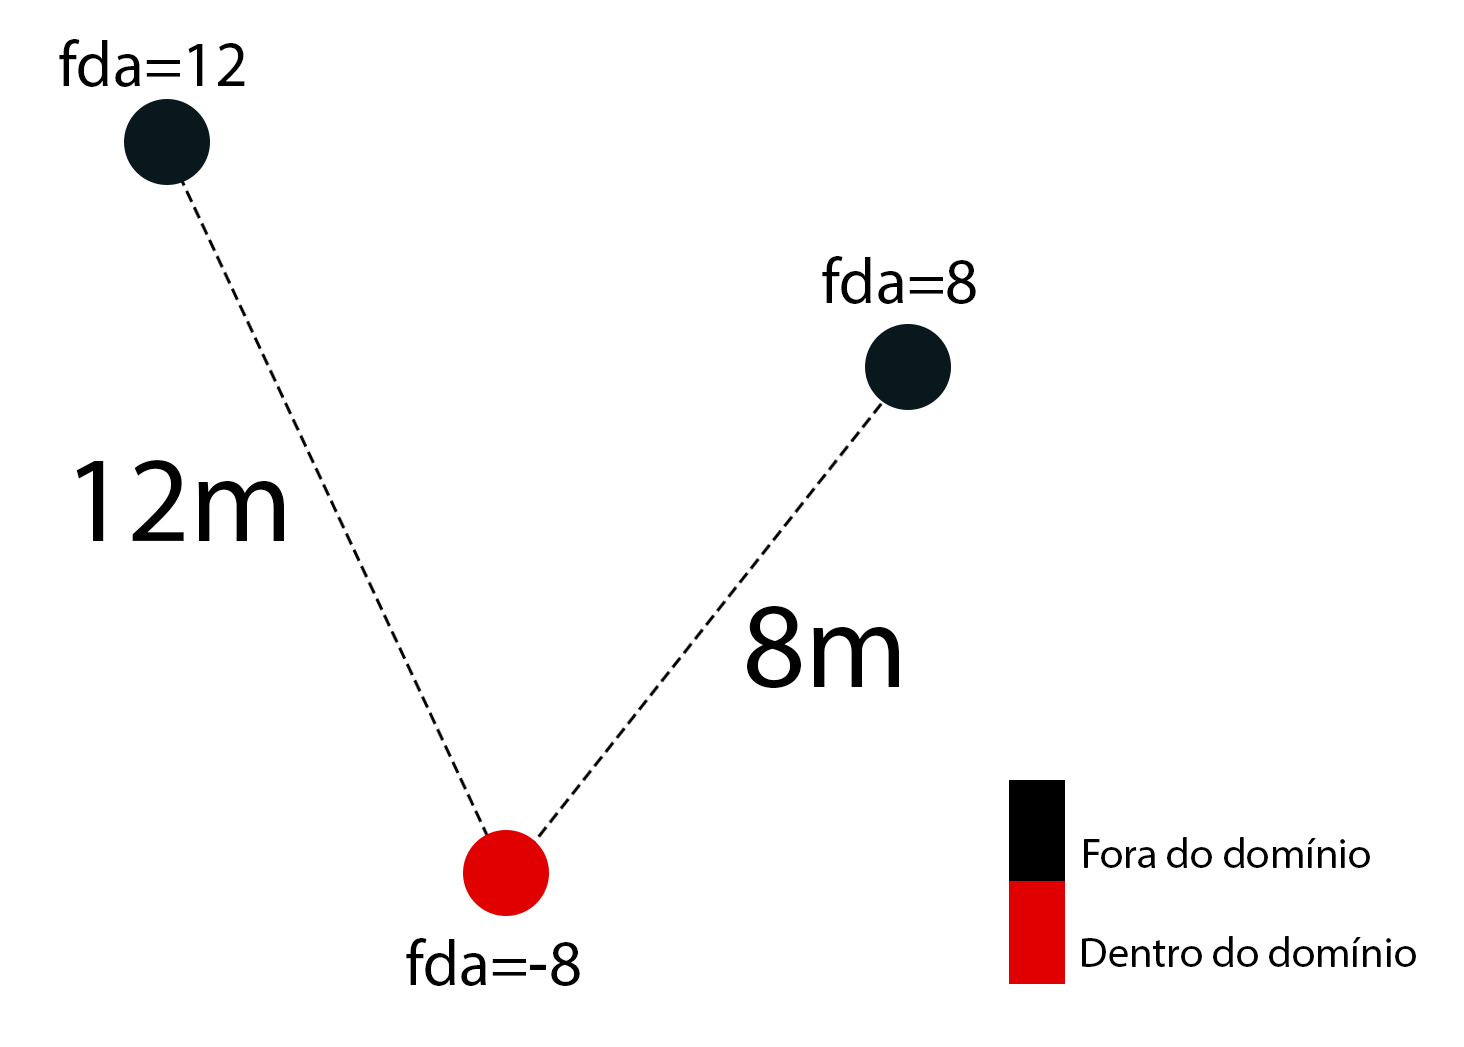
\includegraphics[width=0.6\textwidth]{capitulo_2/2d_ex.jpg}
	\end{center}
	%\legend{Modificado de \citeonline{martin2017implicitmodeling}}
\end{figure}

Desse modo, o valor da função distância assinalada $d_k$ para a o domínio $k$ modelado no local $u_\alpha$ é:

\begin{equation}
	d_k(u_\alpha)=\begin{cases}
	-\parallel u_\alpha-u_\beta\parallel,\:\textrm{se $u_\alpha$ pertence ao domínio}\\
	+\parallel u_\alpha-u_\beta\parallel,\:\textrm{se $u_\alpha$ não pertence ao domínio}\end{cases}
    \label{eq_mult_sg}
\end{equation}

O local $u_\beta$ corresponde à amostra mais próxima codificada com um indicador diferente de $u_\alpha$.

A função distância assinalada calculada para cada umas das categorias do banco de dados é vista na \autoref{indcalc}.

\begin{figure}
    \caption{Distâncias assinaladas calculadas para cada uma das categorias do banco de dados.} \label{indcalc}
     \centering
     \subfloat[][Categoria 1]{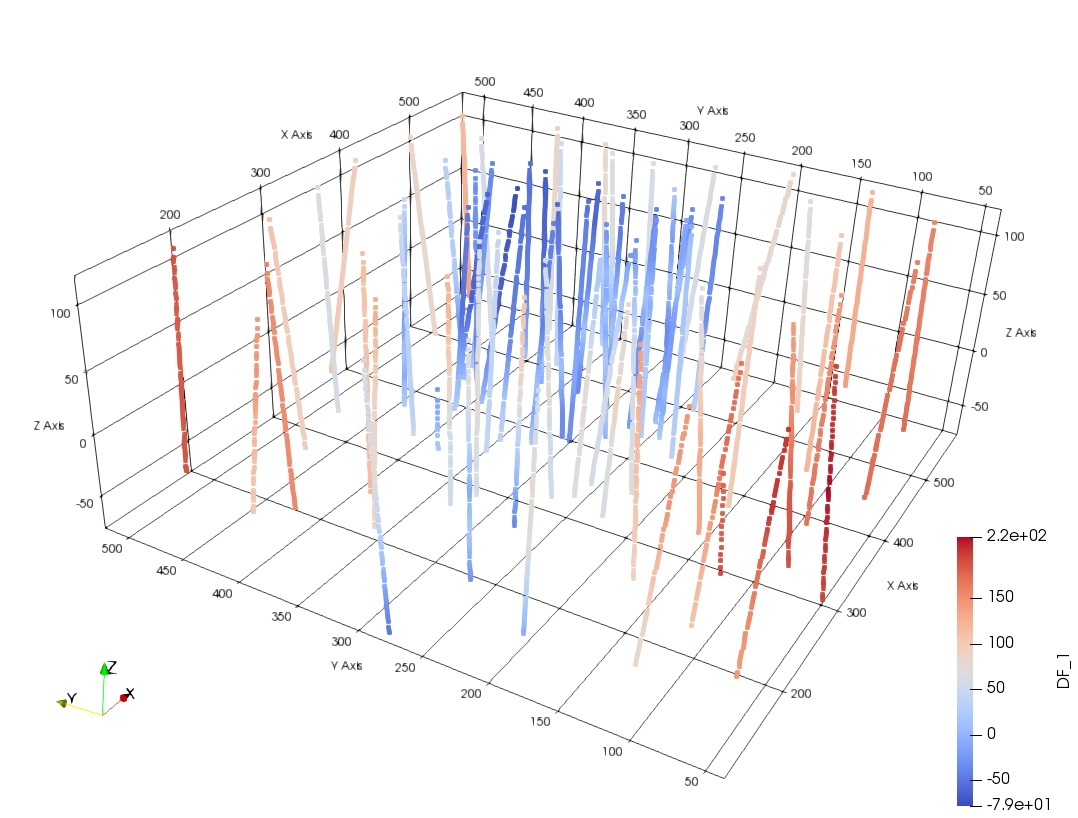
\includegraphics[width=.3\textwidth]{capitulo_2/df1.jpeg}\label{<figure1>}}
     \subfloat[][Categoria 2]{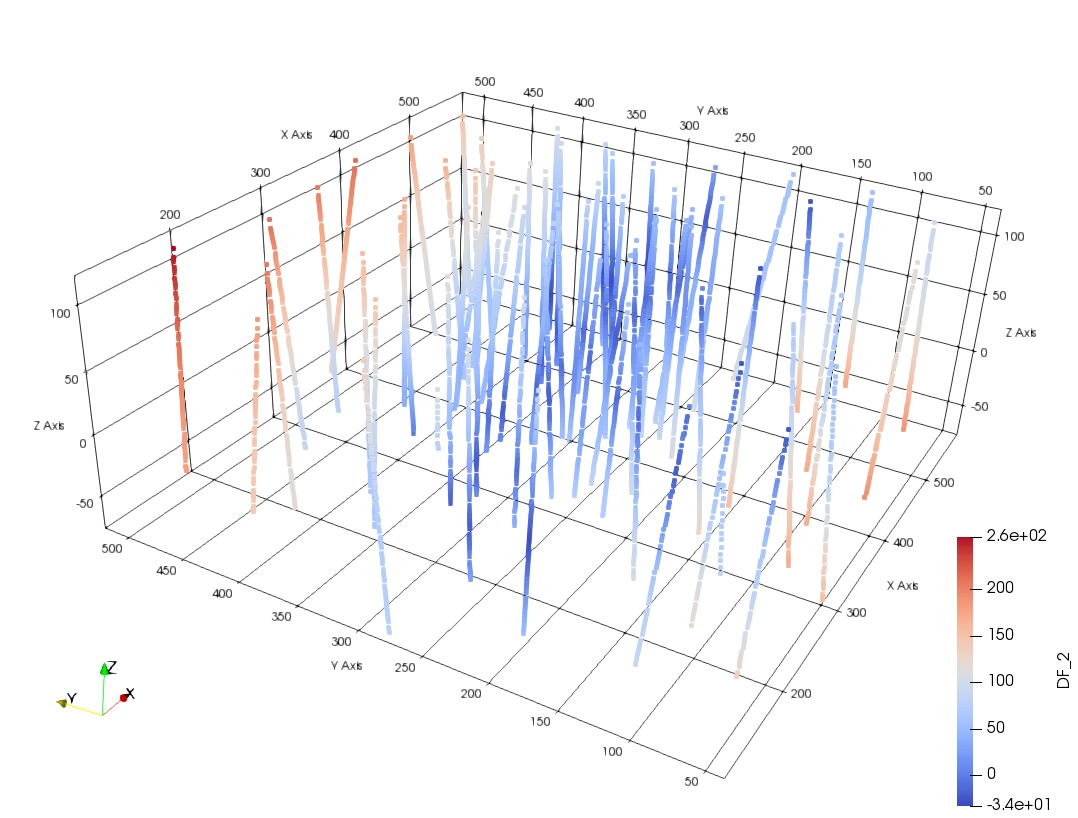
\includegraphics[width=.3\textwidth]{capitulo_2/df2.jpeg}\label{<figure2>}}
     \subfloat[][Categoria 3]{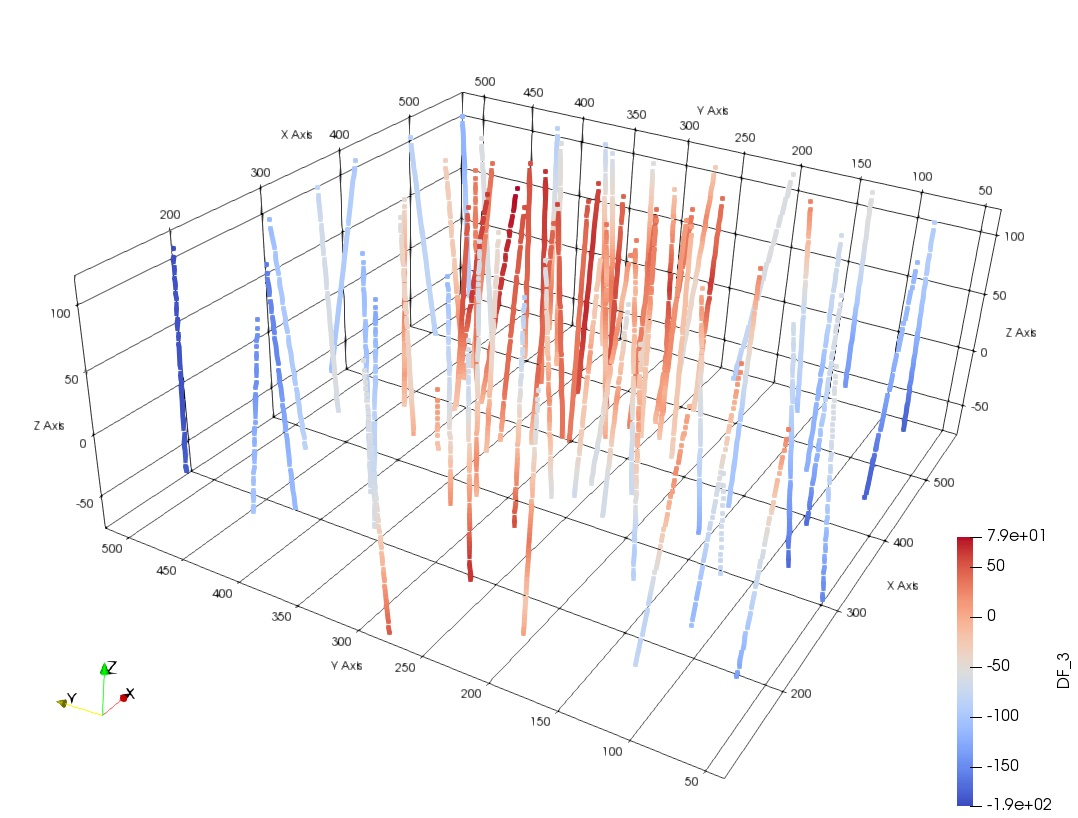
\includegraphics[width=.3\textwidth]{capitulo_2/df3.jpeg}\label{<figure2>}}
\end{figure}

Para corpos geológicos que se estendem muito mais em uma direção em relação às demais, como os corpos tabulares por exemplo, as distâncias calculadas podem ser anisotrópicas. Sendo assim, as coordenadas originais $x$, $y$ e $z$ dos dados devem ser rotacionadas e/ou contraídas/dilatadas, a partir da transformação da \autoref{eq_rot_matrix}. Então, as distâncias euclideanas (\autoref{eq_mult_sg}) são calculadas normalmente para as novas coordenadas $x''$, $y''$, $z''$.

\begin{equation}
\resizebox{.9 \textwidth}{!}{%
$
\begin{bmatrix} x'' \\ y'' \\ z'' \end{bmatrix} = \begin{bmatrix} \frac{1}{a_{max}} & 0 & 0 \\ 0 & \frac{1}{a_{min}} & 0 \\ 0 & 0 & \frac{1}{a_{vert}} \end{bmatrix} \\ \begin{bmatrix}\cos\alpha\cos\phi-\sin\alpha\sin\beta\sin\phi & -\sin\alpha\cos\phi-\cos\alpha\sin\beta\sin\phi & \cos\beta\sin\phi \\ \sin\alpha\cos\beta & \cos\alpha\cos\beta & \sin\beta \\ -\cos\alpha\sin\phi-\sin\alpha\sin\beta\cos\phi & \sin\alpha\sin\phi-\cos\alpha\sin\beta\cos\phi & \cos\beta\cos\phi \end{bmatrix} \begin{bmatrix} x \\ y \\ z \end{bmatrix}
$
}
\label{eq_rot_matrix}
\end{equation}

Onde $a_{max}$, $a_{min}$ e $a_{vert}$ são as dimensões dos eixos máximo, médio e mínimo de anisotropia, e $\alpha$, $\beta$ e $\phi$, os ângulos de azimute, mergulho e \textit{rake}, respectivamente.

\section{Variografia das distâncias calculadas}

No caso das distâncias assinaladas, obter um modelo de covariância a partir dos variogramas experimentais não é trivial. Distâncias assinaladas não são estacionárias, o variograma não se estabiliza em um patamar. Além disso, o caráter extremamente contínuo das distâncias torna a identificação analítica das direções principais um processo embaraçoso.

\citeonline{manchuck_deutsch_Geometric} sugerem alternativas para modelagem do variograma das distâncias:

\begin{itemize}
    \item Treinar o variograma usando validação cruzada;
    \item Tentar modelar interativamente os variogramas experimentais;
    \item Calcular e modelar os variogramas para as propriedades de indicadores e transformá-los em um equivalente gaussiano para as distâncias assinaladas;
    \item inferir um modelo de covariância plausível a partir de mapas delineados a mão.
\end{itemize}

O alcance do variograma, juntamente com a anisotropia, controlam a extensão e forma dos domínios modelados. Os variogramas experimentais das distâncias assinaladas nunca exibem efeito pepita. Porém, pode ser adicionado arbitrariamente pelo usuário para controlar a interconectividade dos domínios, adicionar ruído ao modelo quando desejável e controlar a extrapolação que pode ser ser excessiva em alguns casos devido à alta continuidade dos modelos Gaussianos.

Os variogramas experimentais das distâncias assinaladas e dos indicadores foram calculados para todas as categorias do banco de dados. A categoria 1 
é uma intrusão vertical. Então foi calculado o variograma omnidirecional no plano horizontal e na direção vertical. A categoria 2 é um intrusão tabular (veio) com direção N351 e mergulho -48. Sendo assim, foi calculado o variograma experimental omnidirecional no plano de atitude e na direção perpendicular ao plano. A categoria 3 é a rocha encaixante, as direções foram as mesmas da categoria 1. A \autoref{par_calc} mostra os parâmetros usados no cálculo dos variogramas experimentais das distâncias assinaladas e dos indicadores.

\begin{table}[]
\centering
\resizebox{\textwidth}{!}{%
\begin{tabular}{cccccc}
Número de lags & Distância do lag & Tolerância linear & Tolerância do azimute & Tolerância do mergulho & Banda horizontal \\ \hline
50            & 5m               & 2.5m              & 90                   & 22.5                  & 20m              \\ \hline
\end{tabular}%
}
\caption{Parâmetros de cálculo dos variogramas experimentais.} \label{par_calc}
\end{table}

O modelo mais indicado para modelar o variograma das distâncias assinaladas é o modelo Gaussiano. A \autoref{sd_var} mostra os variogramas experimentais e modelos ajustados das distâncias assinaladas para cada uma das categorias do banco de dados. Os modelos foram ajustados de forma automática pelo software PyGeostat, com efeito pepita de 0.01 (para evitar instabilidades nas matrizes de krigagem), uma estrutura Gaussiana, patamar estandardizado e com um máximo de 2500 iterações.  

\begin{figure} 
\caption{Variogramas experimentais das distâncias assinaladas e modelos para cada uma das categorias do banco de dados.} \label{sd_var}
     \centering
     \subfloat[][Categoria 1]{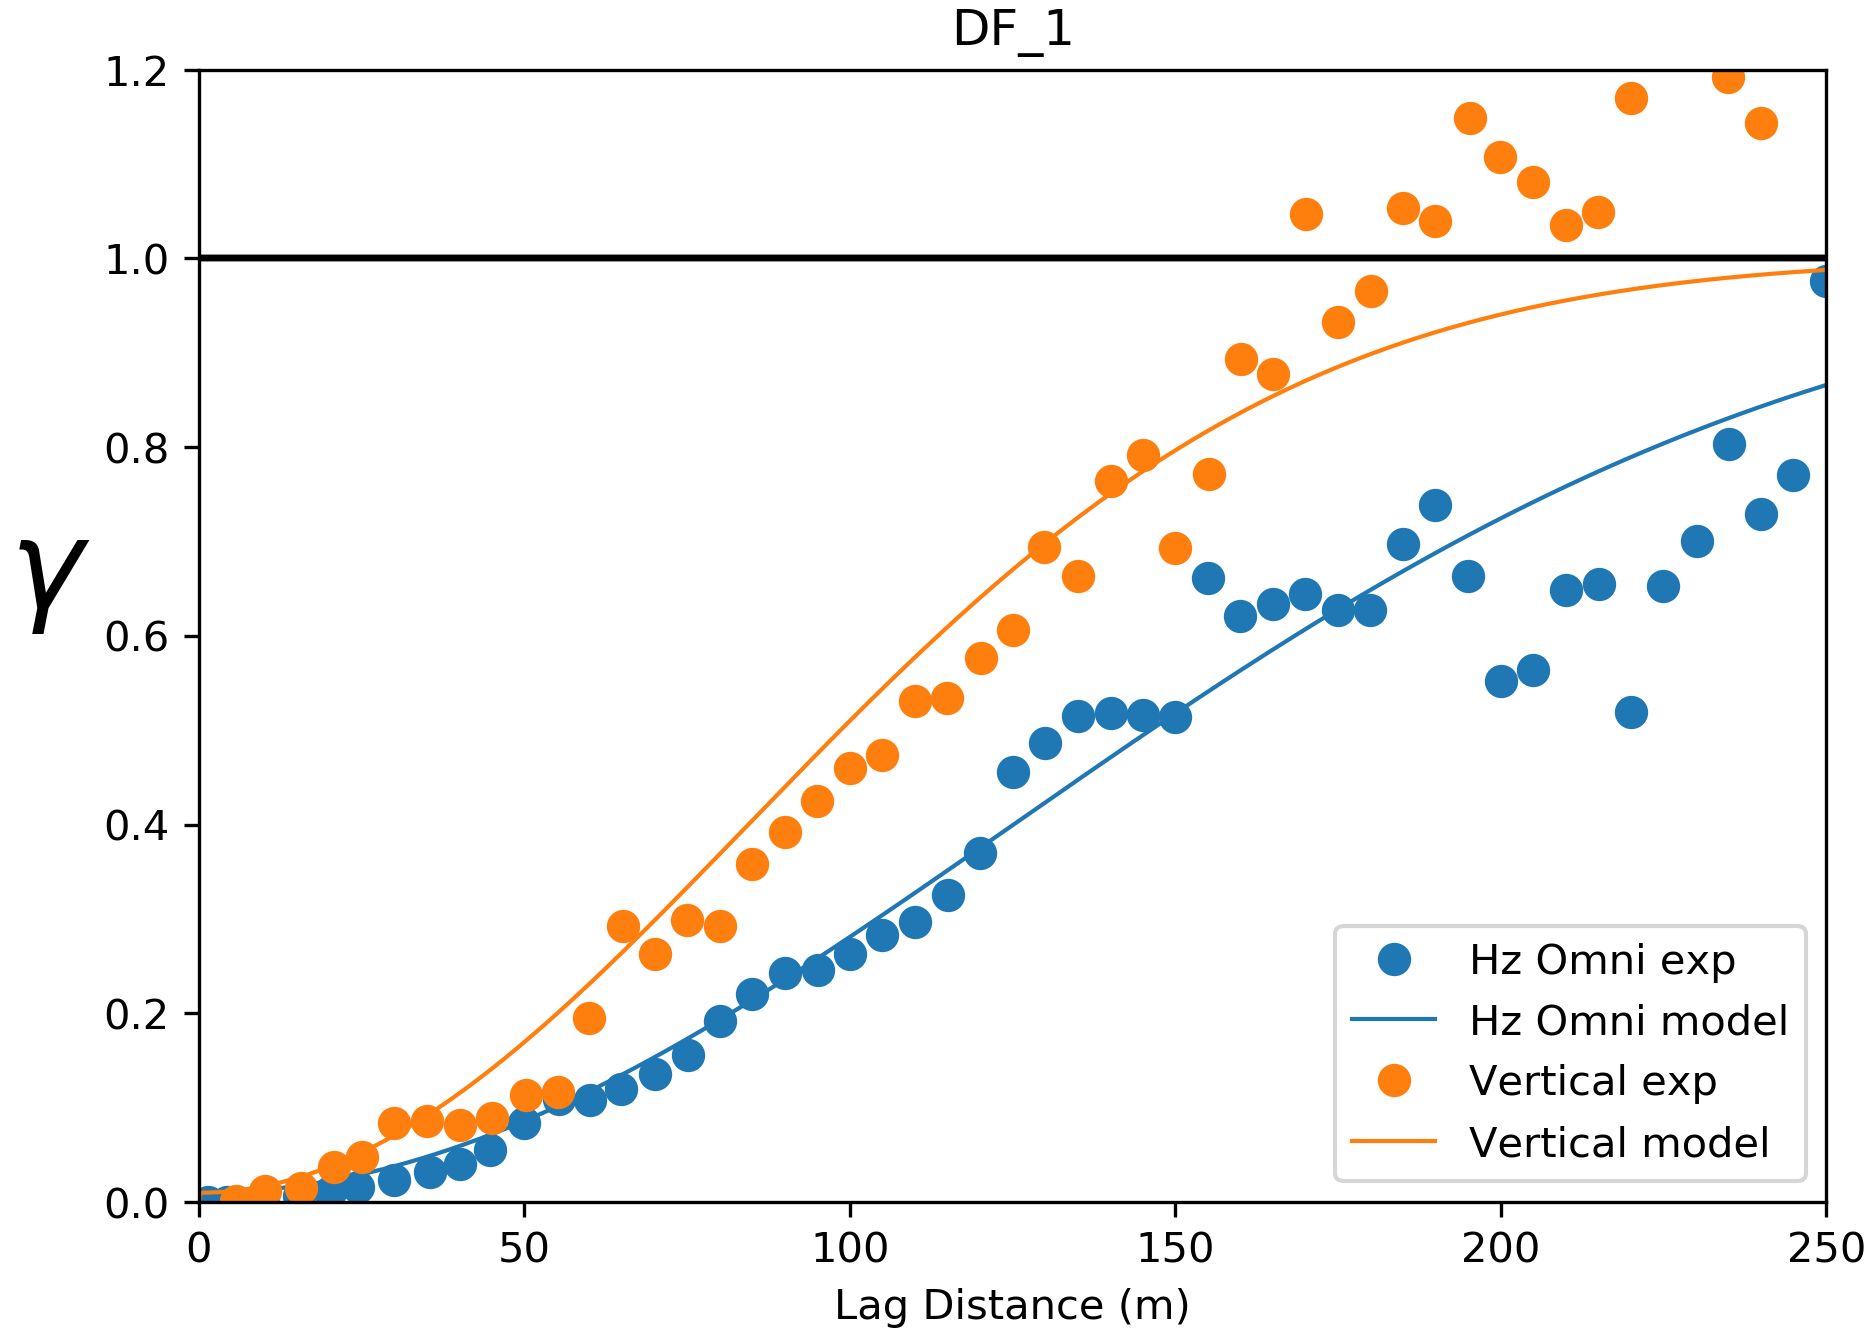
\includegraphics[width=.3\textwidth]{capitulo_2/var_DF_1.png}\label{<figure1>}}
     \subfloat[][Categoria 2]{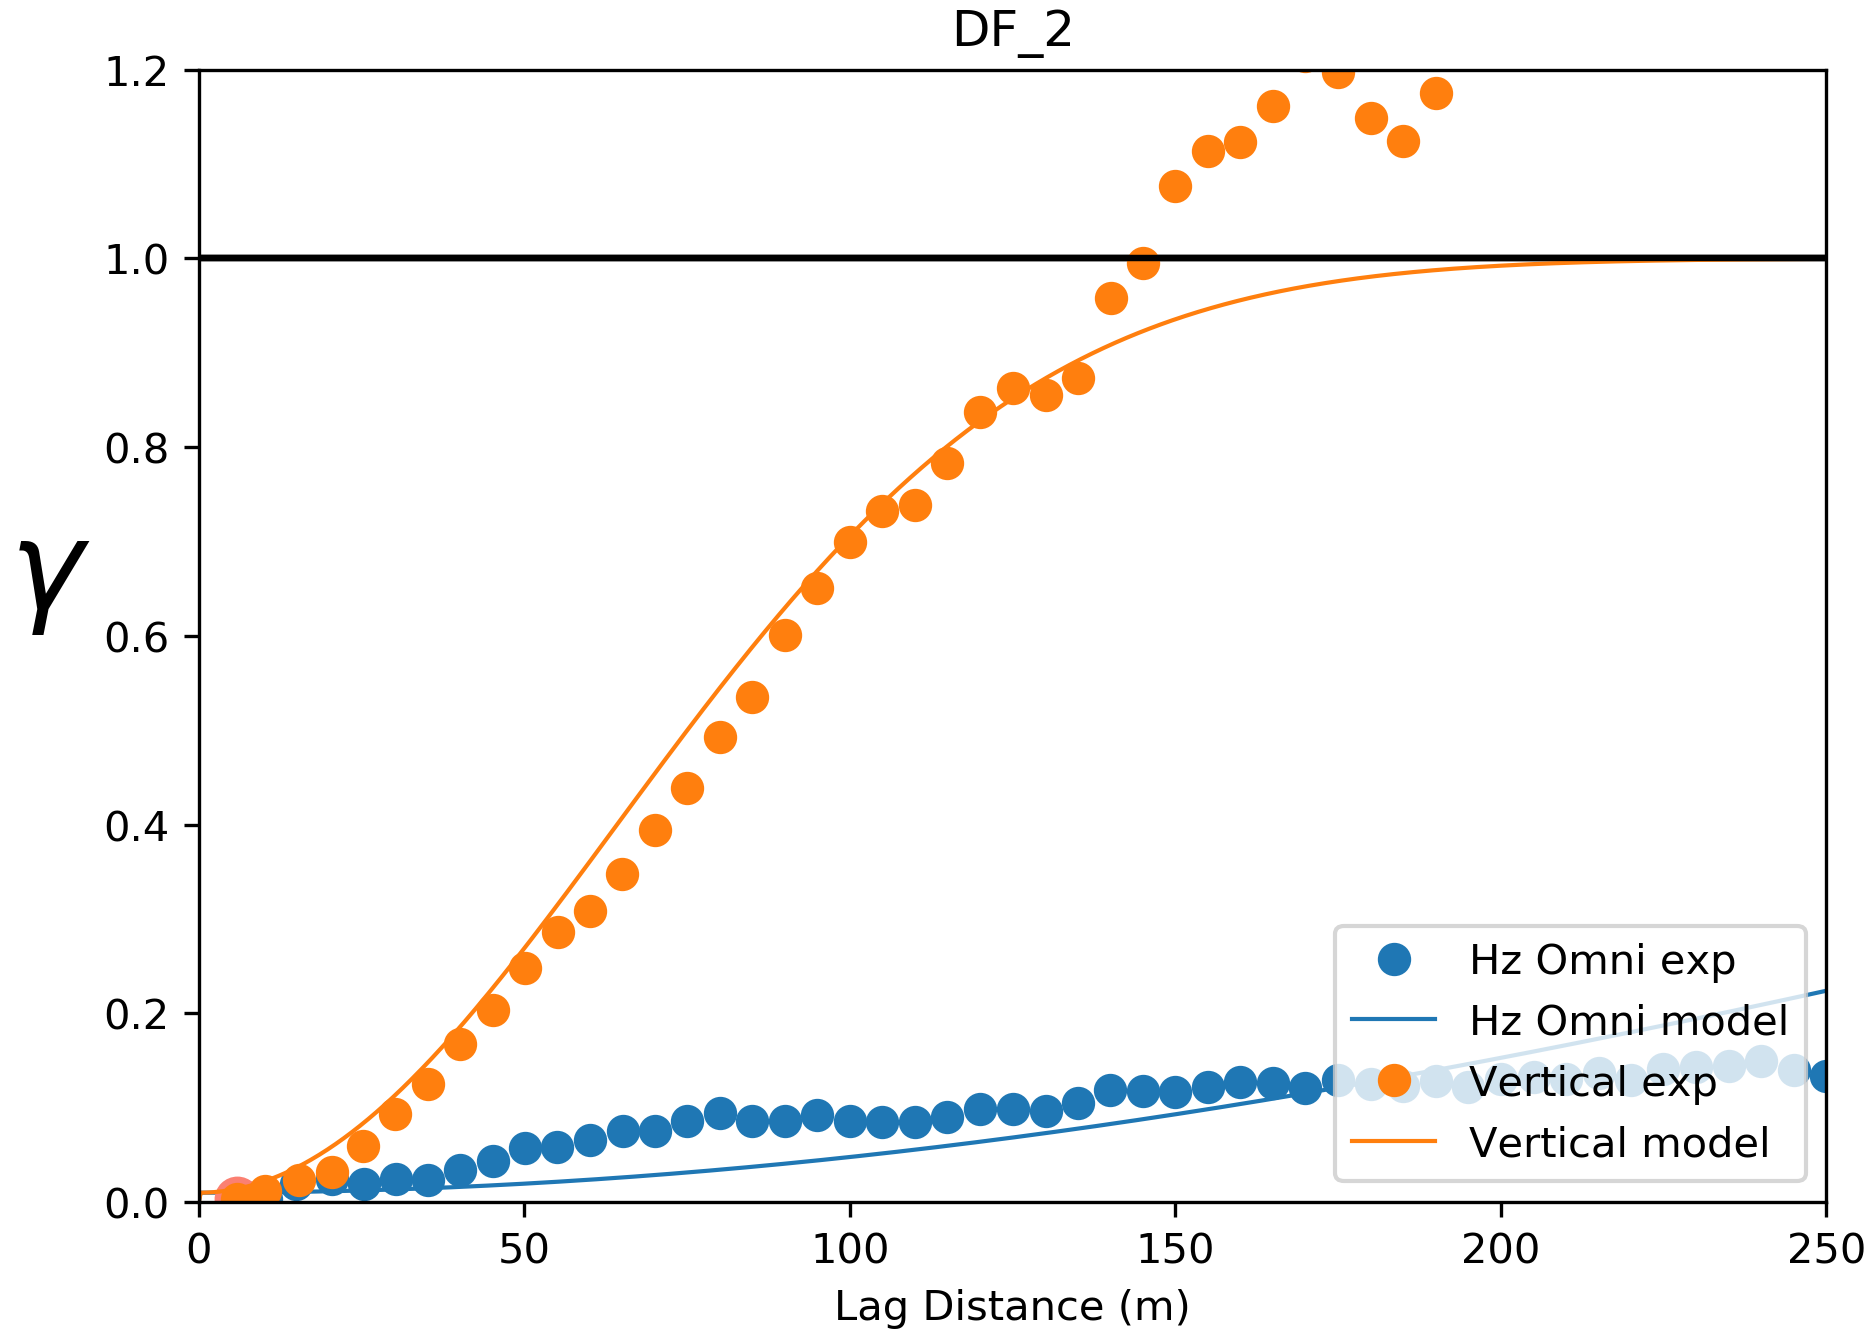
\includegraphics[width=.3\textwidth]{capitulo_2/var_DF_2.png}\label{<figure2>}}
     \subfloat[][Categoria 3]{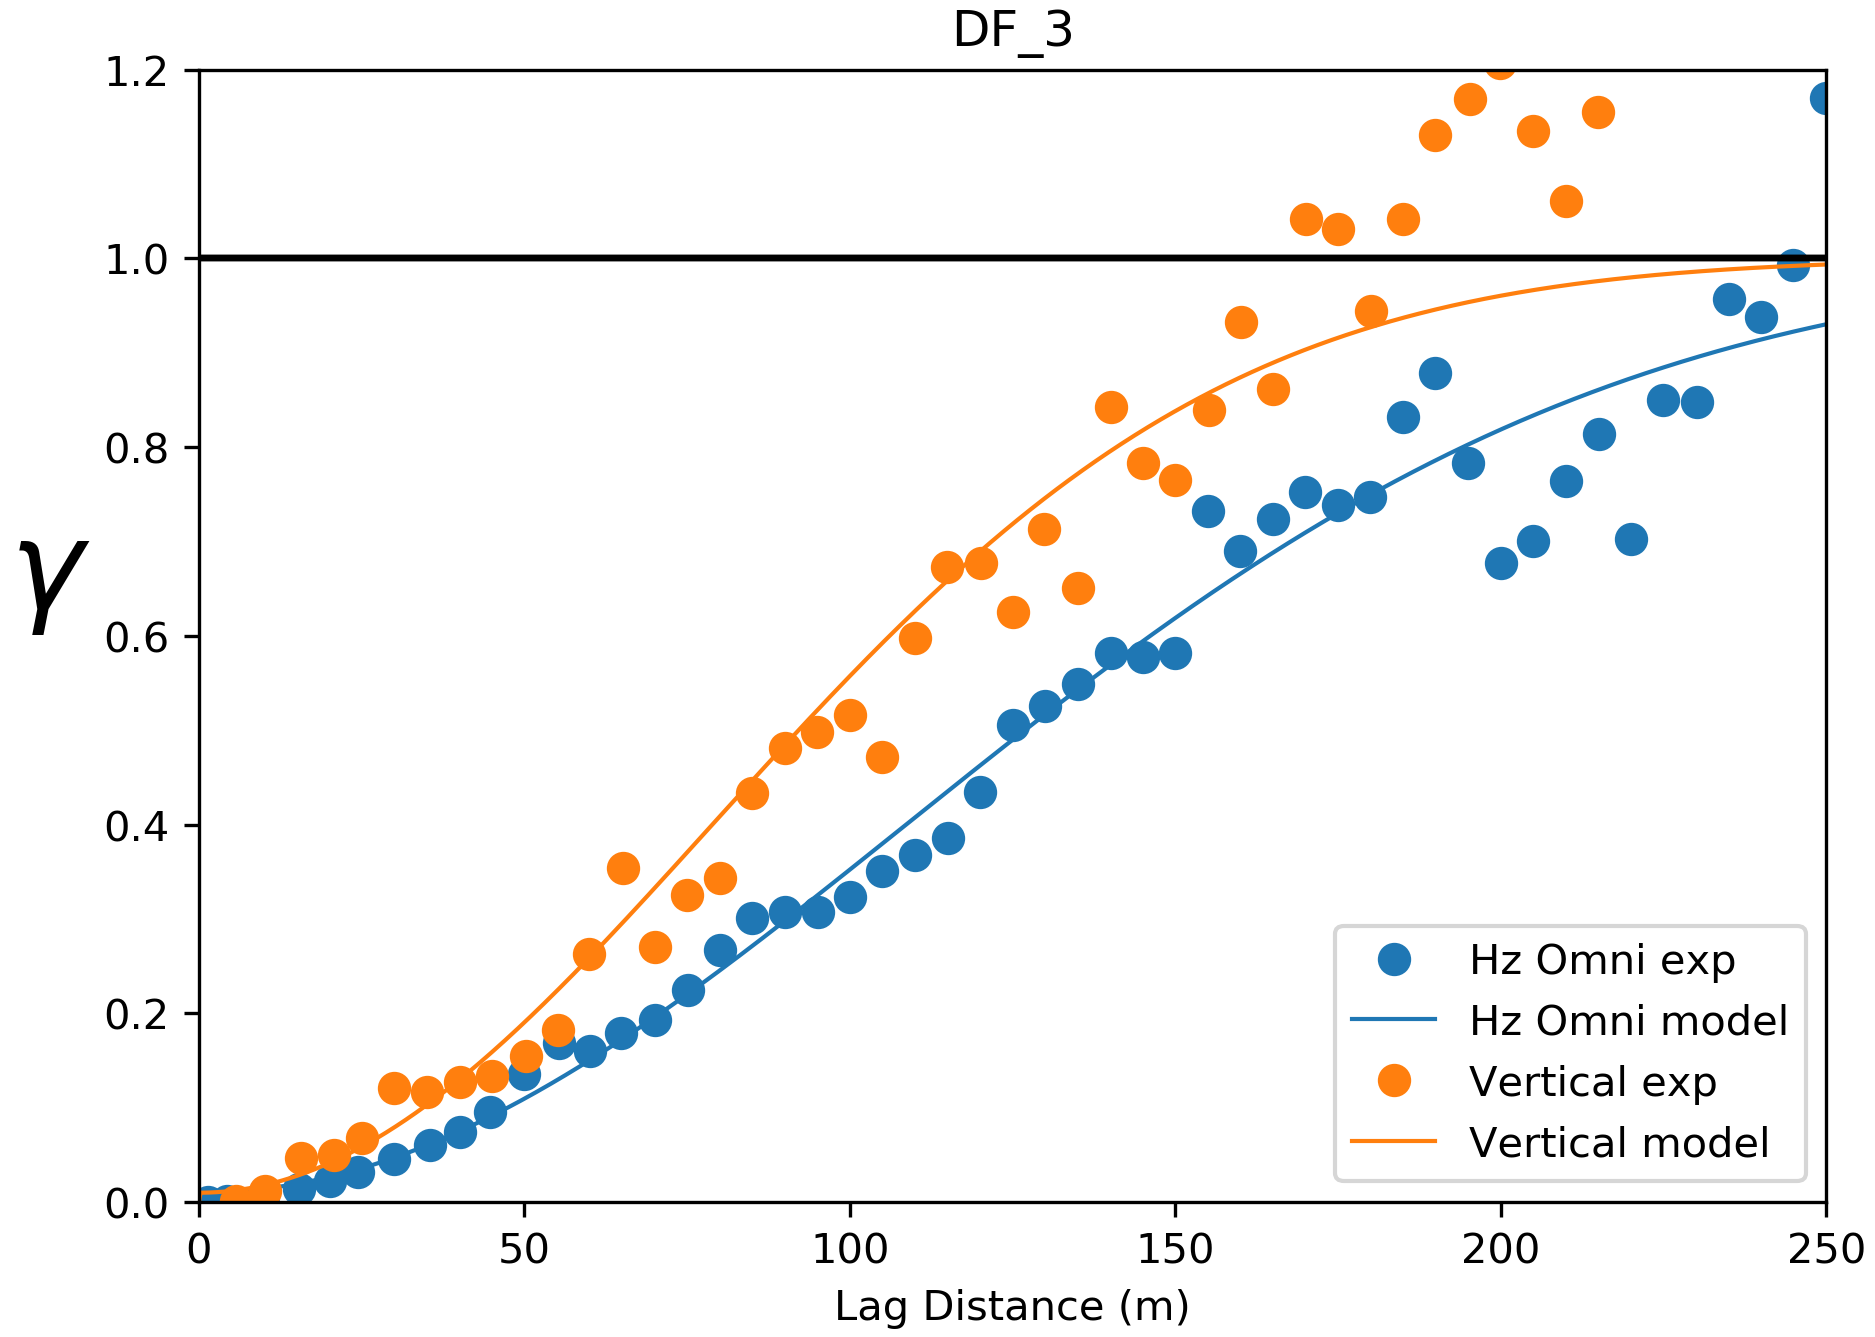
\includegraphics[width=.3\textwidth]{capitulo_2/var_DF_3.png}\label{<figure2>}}
\end{figure}

Os modelos variográficos para cada categoria são expressos pelas \autoref{varsd1}, \autoref{varsd2} e \autoref{varsd3}.

\begin{equation}
\label{varsd1}
\gamma_{SD1}(h)=0.01+0.99gauss\left(\frac{h_{omni}}{306m}, \frac{h_{normal}}{206m}\right)
\end{equation}

\begin{equation}
\label{varsd2}
\gamma_{SD2}(h)=0.01+0.99gauss\left(\frac{h_{omni}}{877m}, \frac{h_{normal}}{157m}\right)
\end{equation}

\begin{equation}
\label{varsd3}
\gamma_{SD3}(h)=0.01+0.99gauss\left(\frac{h_{omni}}{265m}, \frac{h_{normal}}{193m}\right)
\end{equation}

O modelo mais indicado para modelar o variograma dos indicadores é o modelo esférico. A \autoref{ind_var} mostra os variogramas experimentais e modelos ajustados para os indicadores de cada uma das categorias do banco de dados. Os modelos foram ajustados de forma automática pelo software PyGeostat, com efeito pepita de 0, uma estrutura esférica, patamar estandardizado e com um máximo de 2500 iterações. 

\begin{figure} 
     \caption{Variogramas experimentais dos indicadores e modelos para cada uma das categorias do banco de dados.} \label{ind_var}
     \centering
     \subfloat[][Categoria 1]{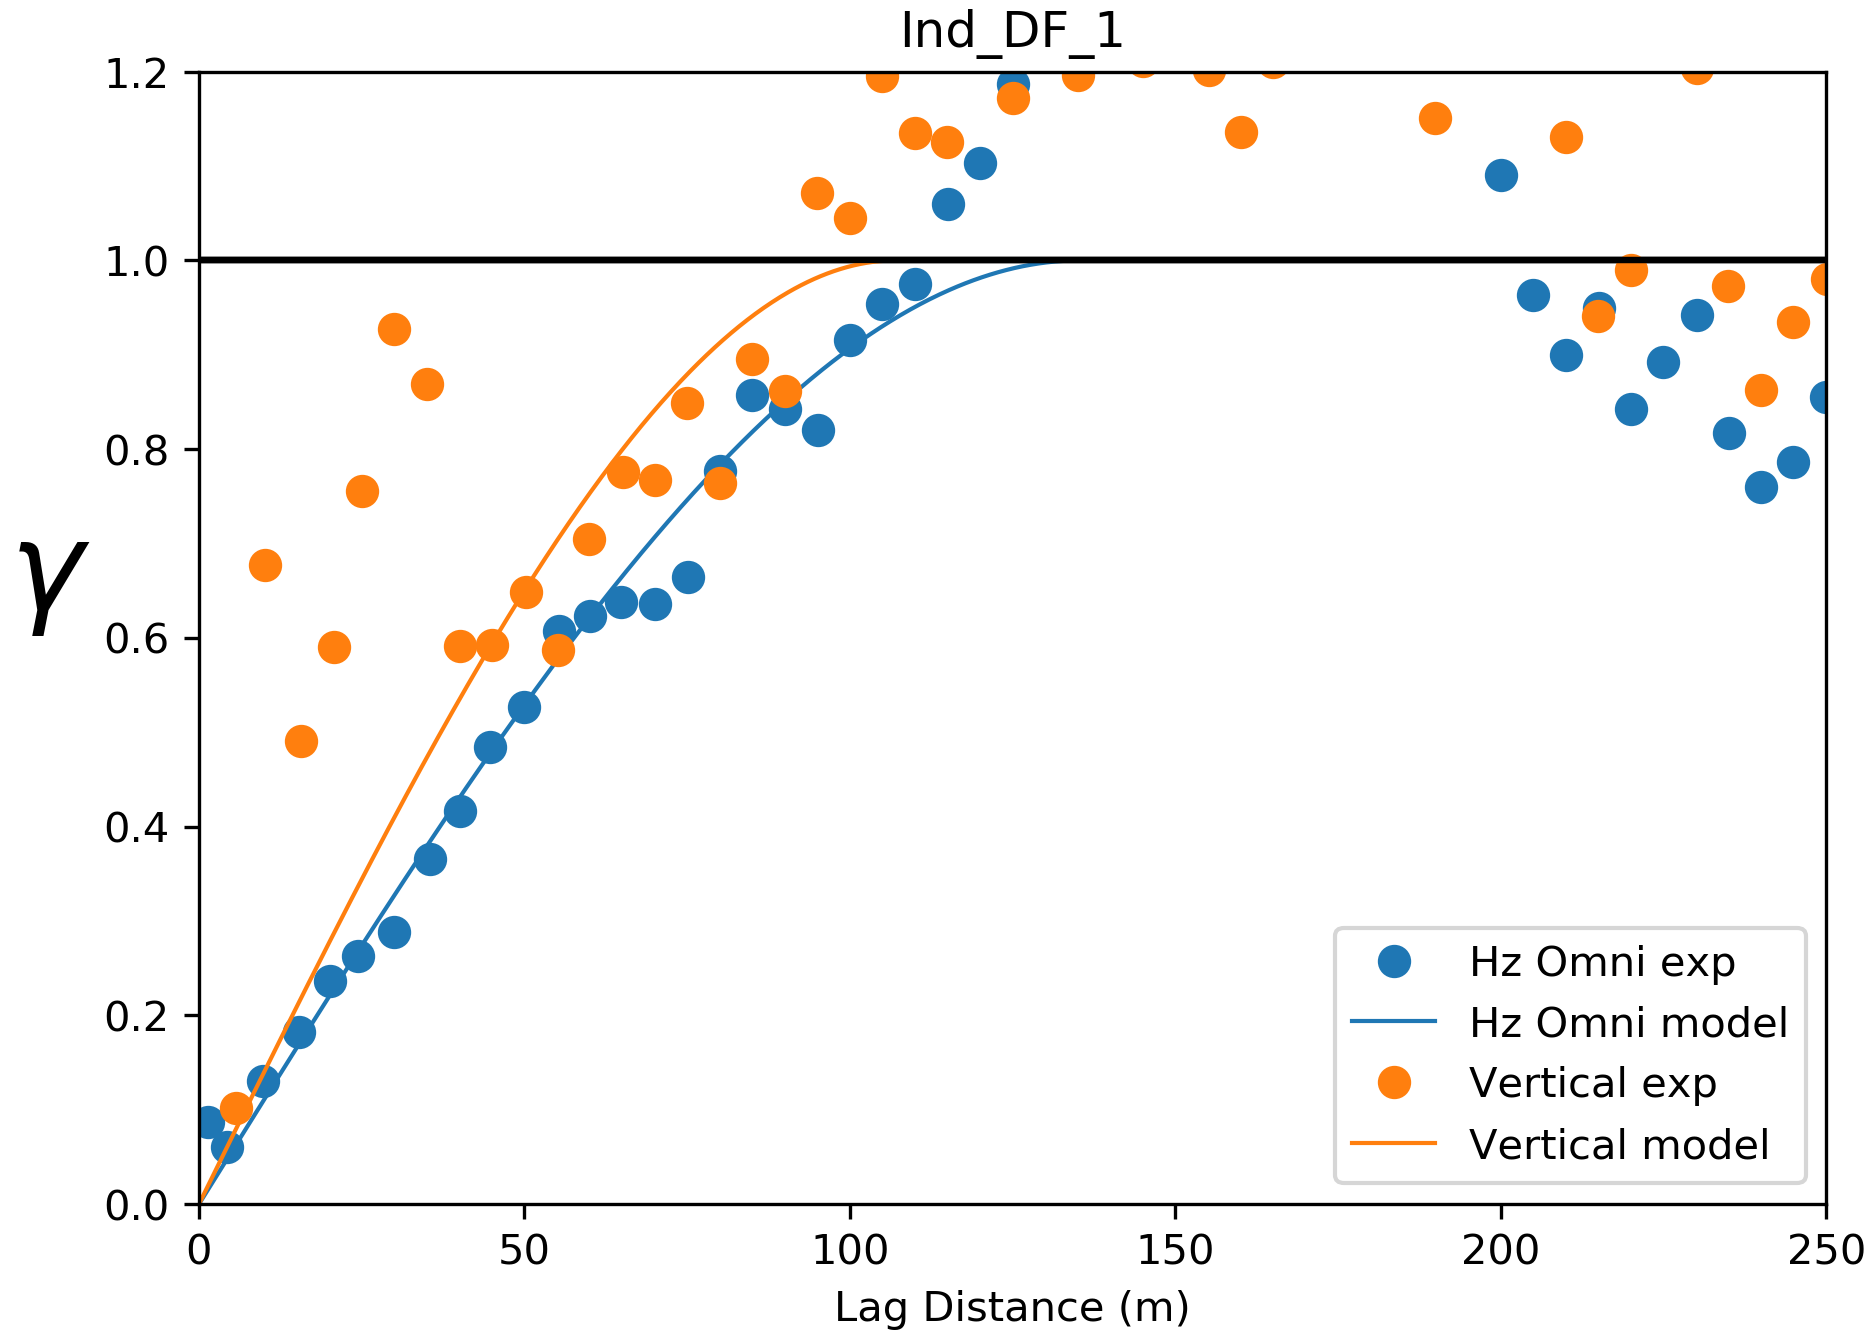
\includegraphics[width=.3\textwidth]{capitulo_2/var_Ind_DF_1.png}\label{<figure1>}}
     \subfloat[][Categoria 2]{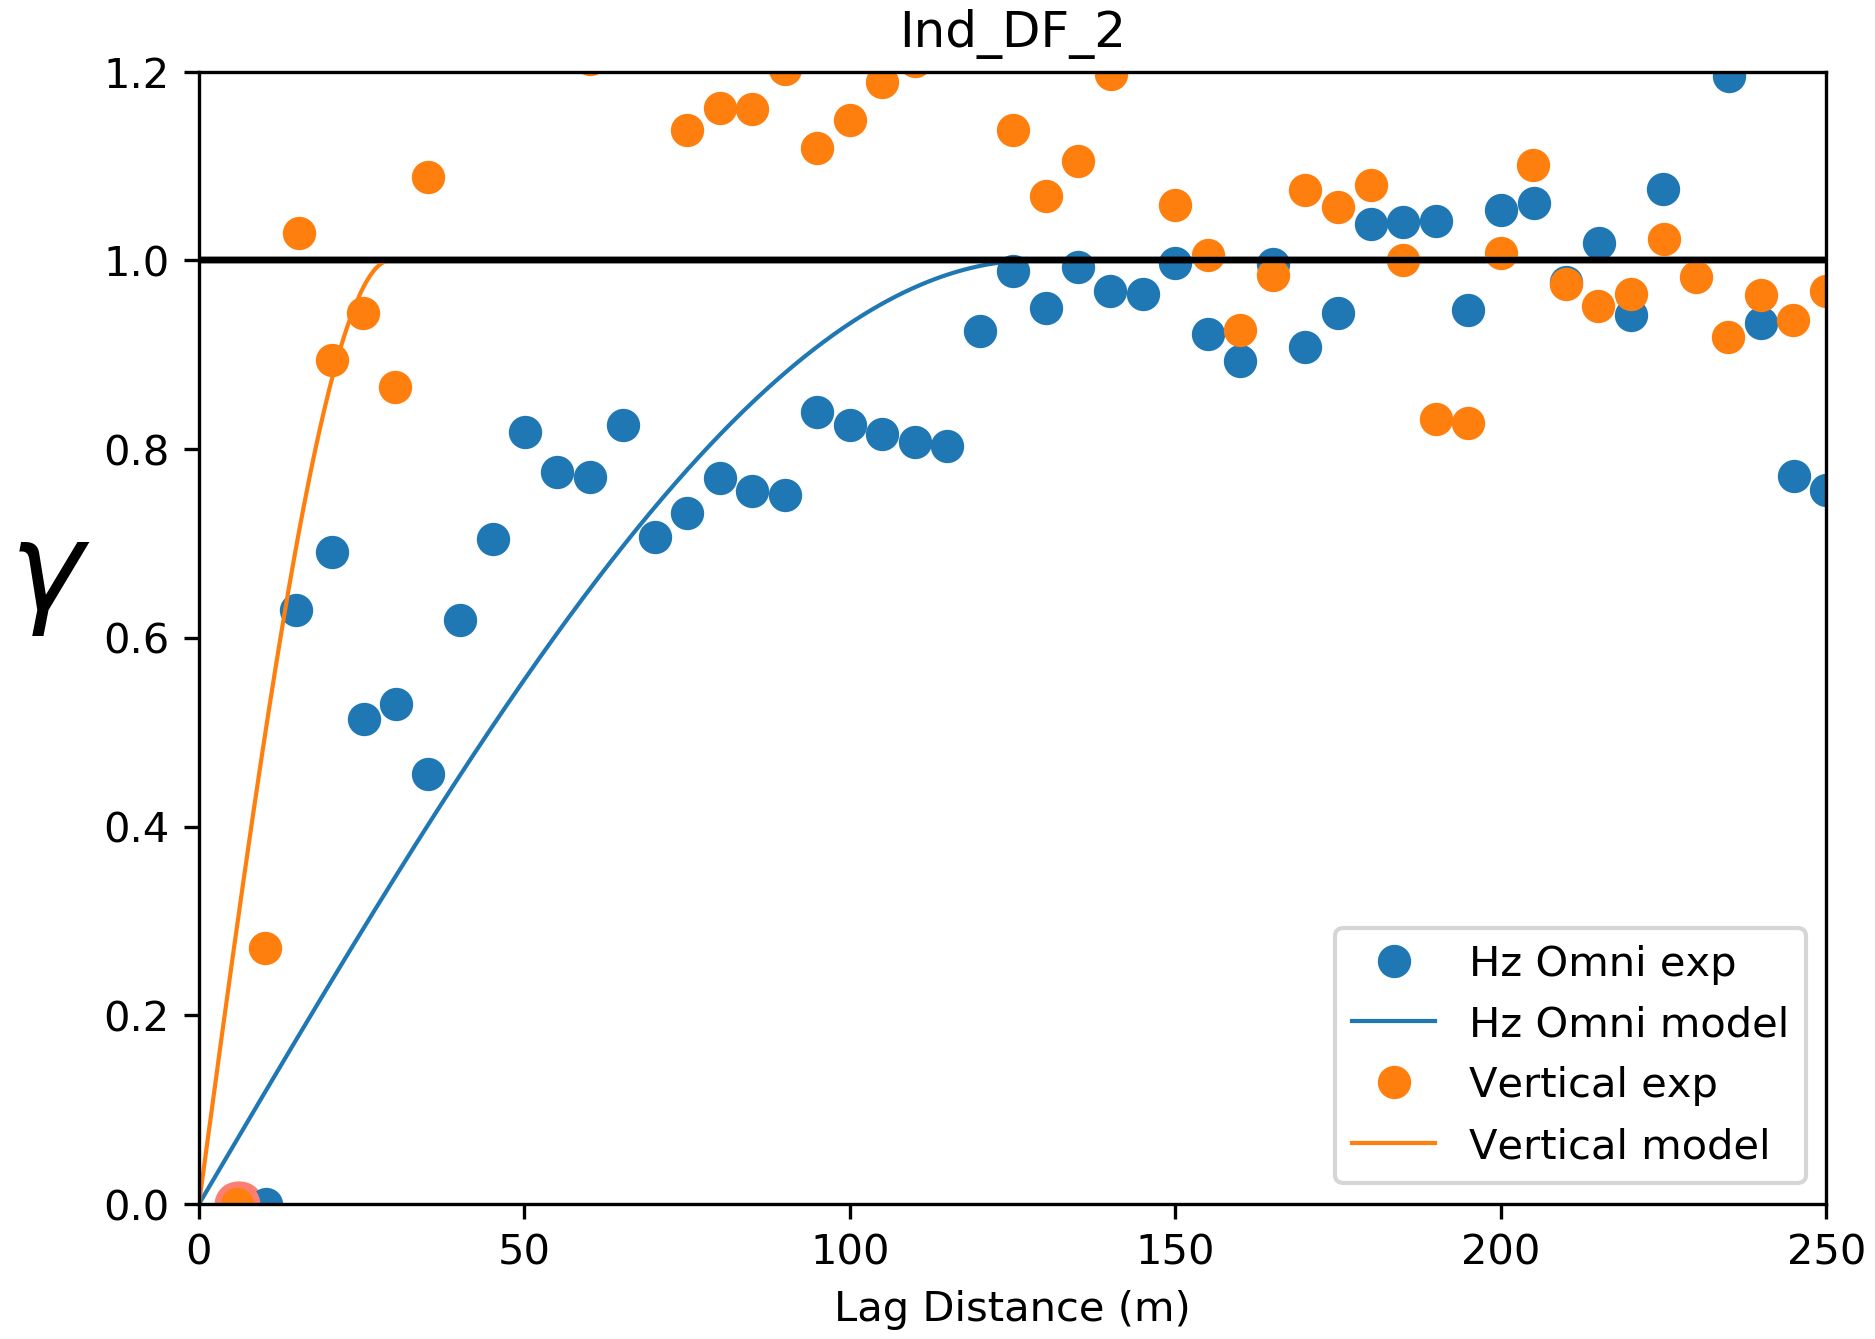
\includegraphics[width=.3\textwidth]{capitulo_2/var_Ind_DF_2.png}\label{<figure2>}}
     \subfloat[][Categoria 3]{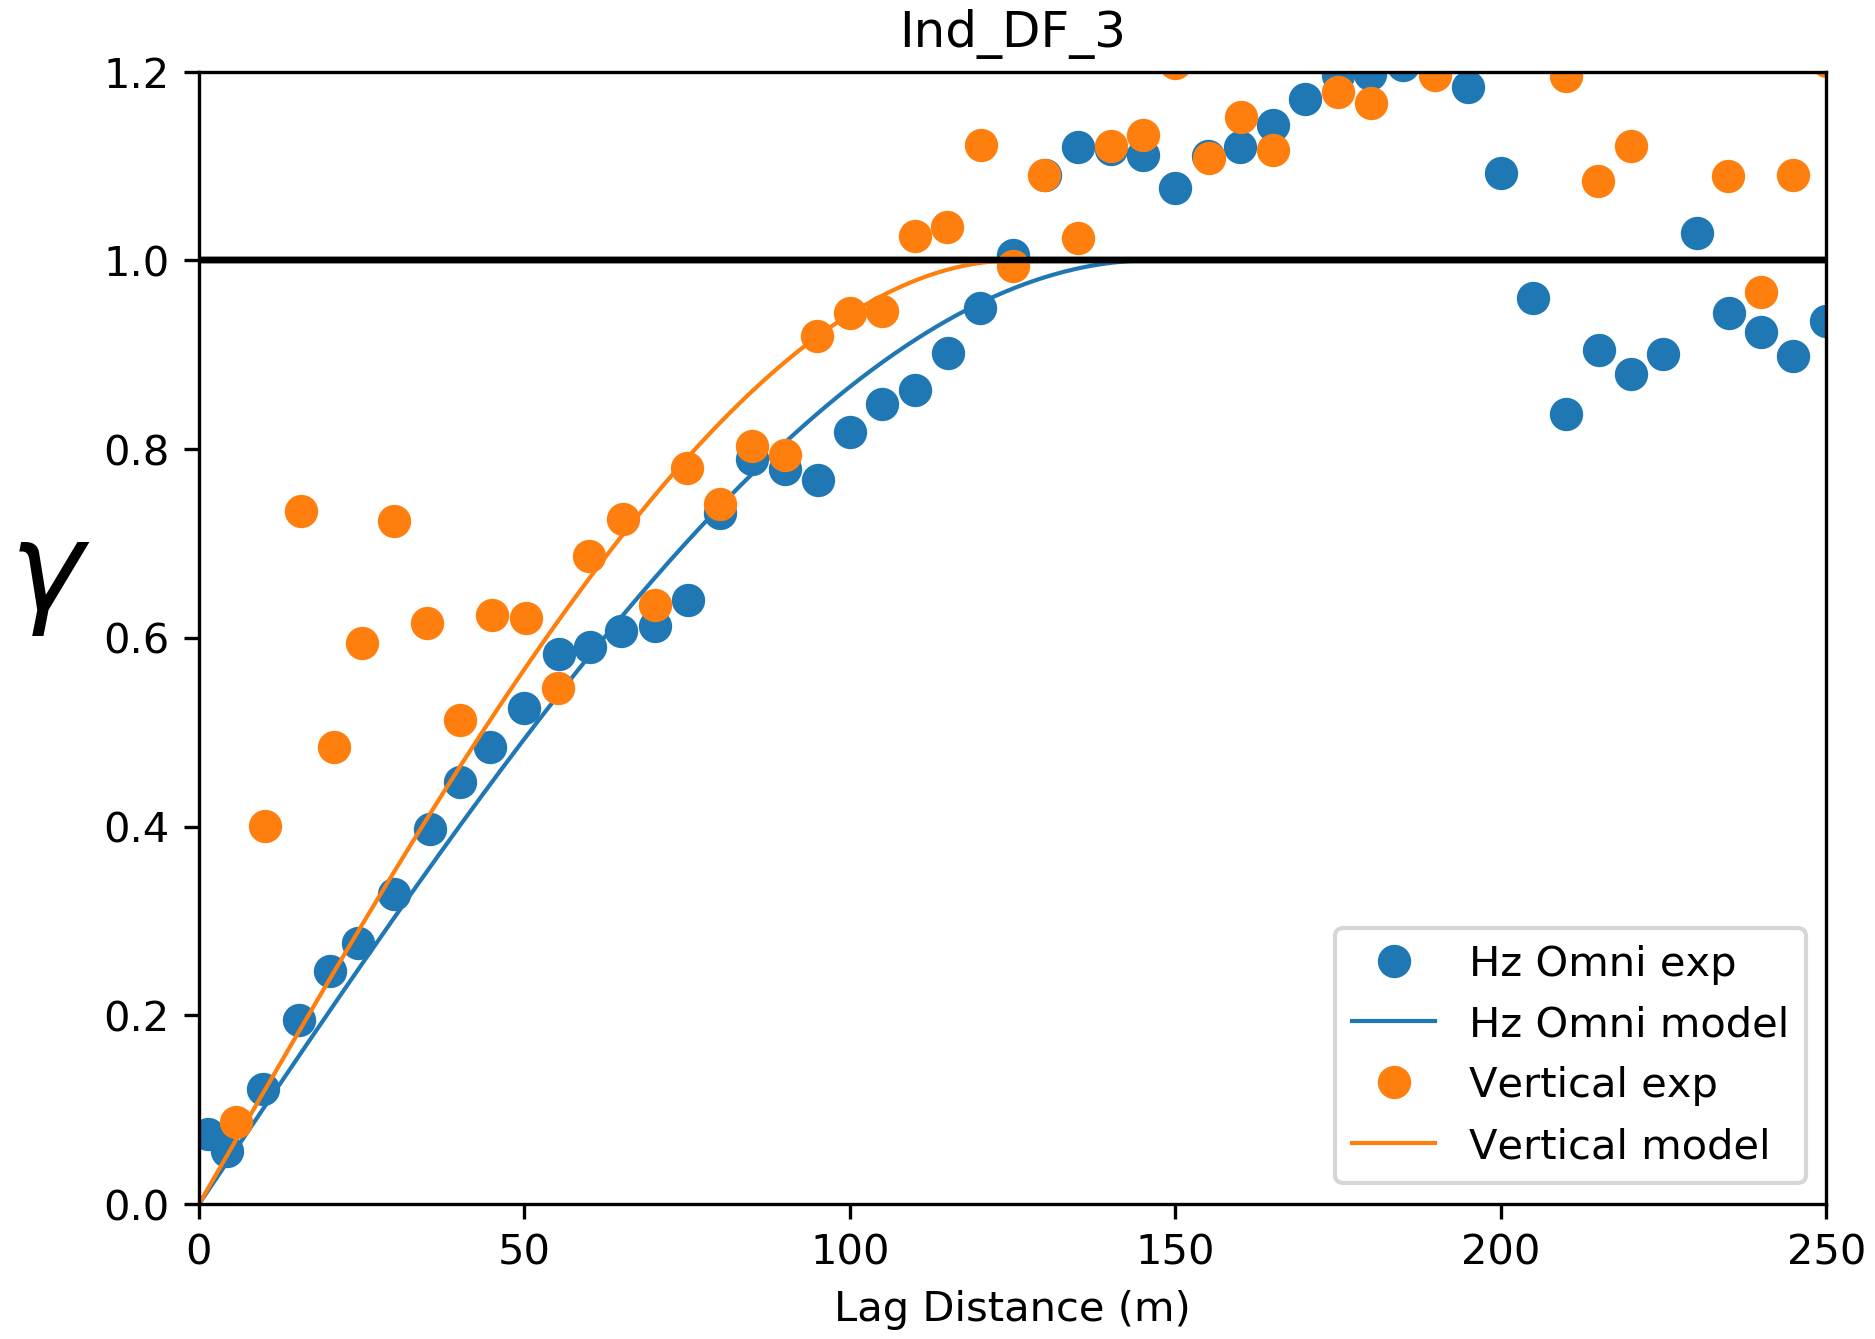
\includegraphics[width=.3\textwidth]{capitulo_2/var_Ind_DF_3.png}\label{<figure2>}}
\end{figure}

Os modelos variográficos para cada categoria são expressos pelas \autoref{varind1}, \autoref{varind2} e \autoref{varind3}.

\begin{equation}
\label{varind1}
\gamma_{IND1}(h)=1.0gauss\left(\frac{h_{omni}}{135m}, \frac{h_{normal}}{106m}\right)
\end{equation}

\begin{equation}
\label{varind2}
\gamma_{IND2}(h)=1.0gauss\left(\frac{h_{omni}}{128m}, \frac{h_{normal}}{29m}\right)
\end{equation}

\begin{equation}
\label{varind3}
\gamma_{IND3}(h)=1.0gauss\left(\frac{h_{omni}}{146m}, \frac{h_{normal}}{125m}\right)
\end{equation}

Em teoria o ajuste dos variogramas dos indicadores é mais fácil se comparado ao variograma das distâncias assinaladas, além de atingirem um patamar, a menor continuidade espacial em relação às distâncias torna a identificação analítica das direções principais um processo mais simples. No entanto, muitas vezes, na prática se observa o contrário.

Uma outra alternativa ao cálculo e modelagem de variogramas é o uso de tabelas de covariância proposto por \citeonline{kloechner_cov_table}, esse estudo propõe a substituição da modelagem tradicional dos variogramas por tabelas de covariância, tornando o processo de modelagem geológica completamente automático e livre da subjetividade do geomodelador. A \autoref{cov_table} mostra o fluxograma da metodologia proposta.

\begin{figure}[!htb]
	\caption{\label{cov_table}Fluxograma da modelagem geológica implícita usando tabelas de covariância.}
	\begin{center}
		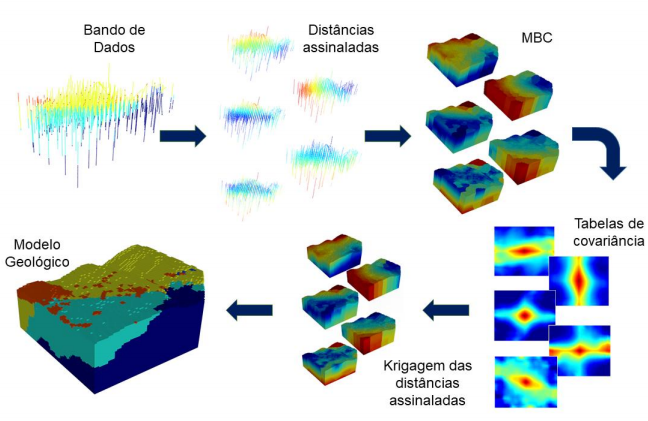
\includegraphics[width=0.7\textwidth]{capitulo_2/cov_table.png}
	\end{center}
	\legend{\citeonline{kloechner_cov_table}}
\end{figure}

O trabalho propõe uma técnica para obter uma tabela de covariância, a partir de um modelo base, que reproduz a continuidade espacial de um dado atributo usando o teorema de convolução via transformada rápida de Fourier. Embora a metodologia tenha apresentado resultados satisfatórios, a construção automática das tabelas de covariância ainda apresenta alguns problemas operacionais que tornam sua aplicação inviável para todos os tipo de depósito.

\section{Interpolação das distâncias calculadas}

Uma vez que as distâncias tenham sido calculadas a partir da localização das amostras, o próximo passo é interpolar o novo banco de dados para o grid definido para a modelagem geológica. Embora métodos implícitos não demandem um grid - são métodos conhecidos como \textit{gridless} - o objetivo final é preencher o grid de estimativas com as categorias correspondentes ou visualizar o modelo através de iso superfícies. Técnicas de extração de iso superfícies exigem a função volumétrica definida exaustivamente em um grid retilíneo  \citeonline{martin2017implicitmodeling}.

\subsection{Resolução do grid}

Para um número constante de amostras, o tempo necessário para interpolação da função volume para todos os nós do grid aumenta linearmente com o número de nós. Os parâmetros do grid de estimativas, muitas vezes, são determinado por requisitos de engenharia do projeto. Todavia, o grid para definição do modelo geológico pode ser diferente do grid definido para os modelos numéricos de teores. A consideração mais importante é a capacidade de reproduzir a menor estrutura geológica de interesse.

Considere os modelos implícitos da \autoref{grid_res} gerados em grids de diferentes resoluções.

\begin{figure}[!htb]
	\caption{\label{grid_res}Efeito da resolução do grid na reprodução de estruturas geológicas.}
	\begin{center}
		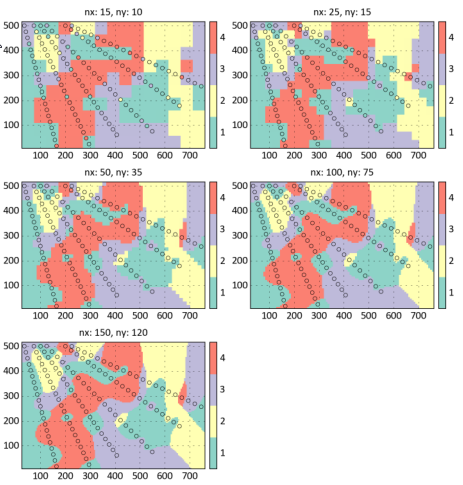
\includegraphics[width=0.6\textwidth]{capitulo_2/grid_res.png}
	\end{center}
	\legend{Fonte: \citeonline{martin2017implicitmodeling}}
\end{figure}

A resolução adequada para esse modelo é entre (nx, ny) = (50, 35) e (nx, ny) = (100, 75). Para os dois primeiros grids há classificação errônea dos nós colocados com amostras, além de (nx, ny) = (100, 75) há pouco benefício na reprodução das estruturas levando em consideração o aumento do tempo de interpolação.

É preciso encontrar um balanço entre resolução e tempo de interpolação. A resolução do grid pode ser aumentada a medida que o projeto avança e mais informação é adquirida \cite{martin2017implicitmodeling}.

Para o estudo de caso foram gerados dois grids com resoluções diferentes, seus parâmetros são mostrados na \autoref{grid_def}.

\begin{table}[]
\centering
\begin{tabular}{lrr}
 & \multicolumn{1}{l}{Grosso} & \multicolumn{1}{l}{Fino} \\ \hline
nx & 49 & 97 \\
ny & 49 & 98 \\
nz & 51 & 102 \\
sx & 10m & 5m \\
sy & 10m & 5m \\
sz & 4m & 2m \\
num & 122451 & 969612 \\ \hline
\end{tabular}
\caption{Parâmetros dos grids de definição dos modelos geológicos implícitos.} \label{grid_def}
\end{table}

A \autoref{dif_res} mostra seções em XZ de dois modelos geológicos implícitos gerados em grids com resoluções diferentes para o banco de dados do estudo de caso. no grid fino (\autoref{a}) as formas reproduzidas são suaves, apresentam realismo geológico, e o número de classificações errôneas é menor.

\begin{figure}[t]
\caption{Modelos geológicos em diferentes resoluções} 
\label{dif_res}
\begin{center}
\subfloat[][Modelo geológico implícto no grid grosso]{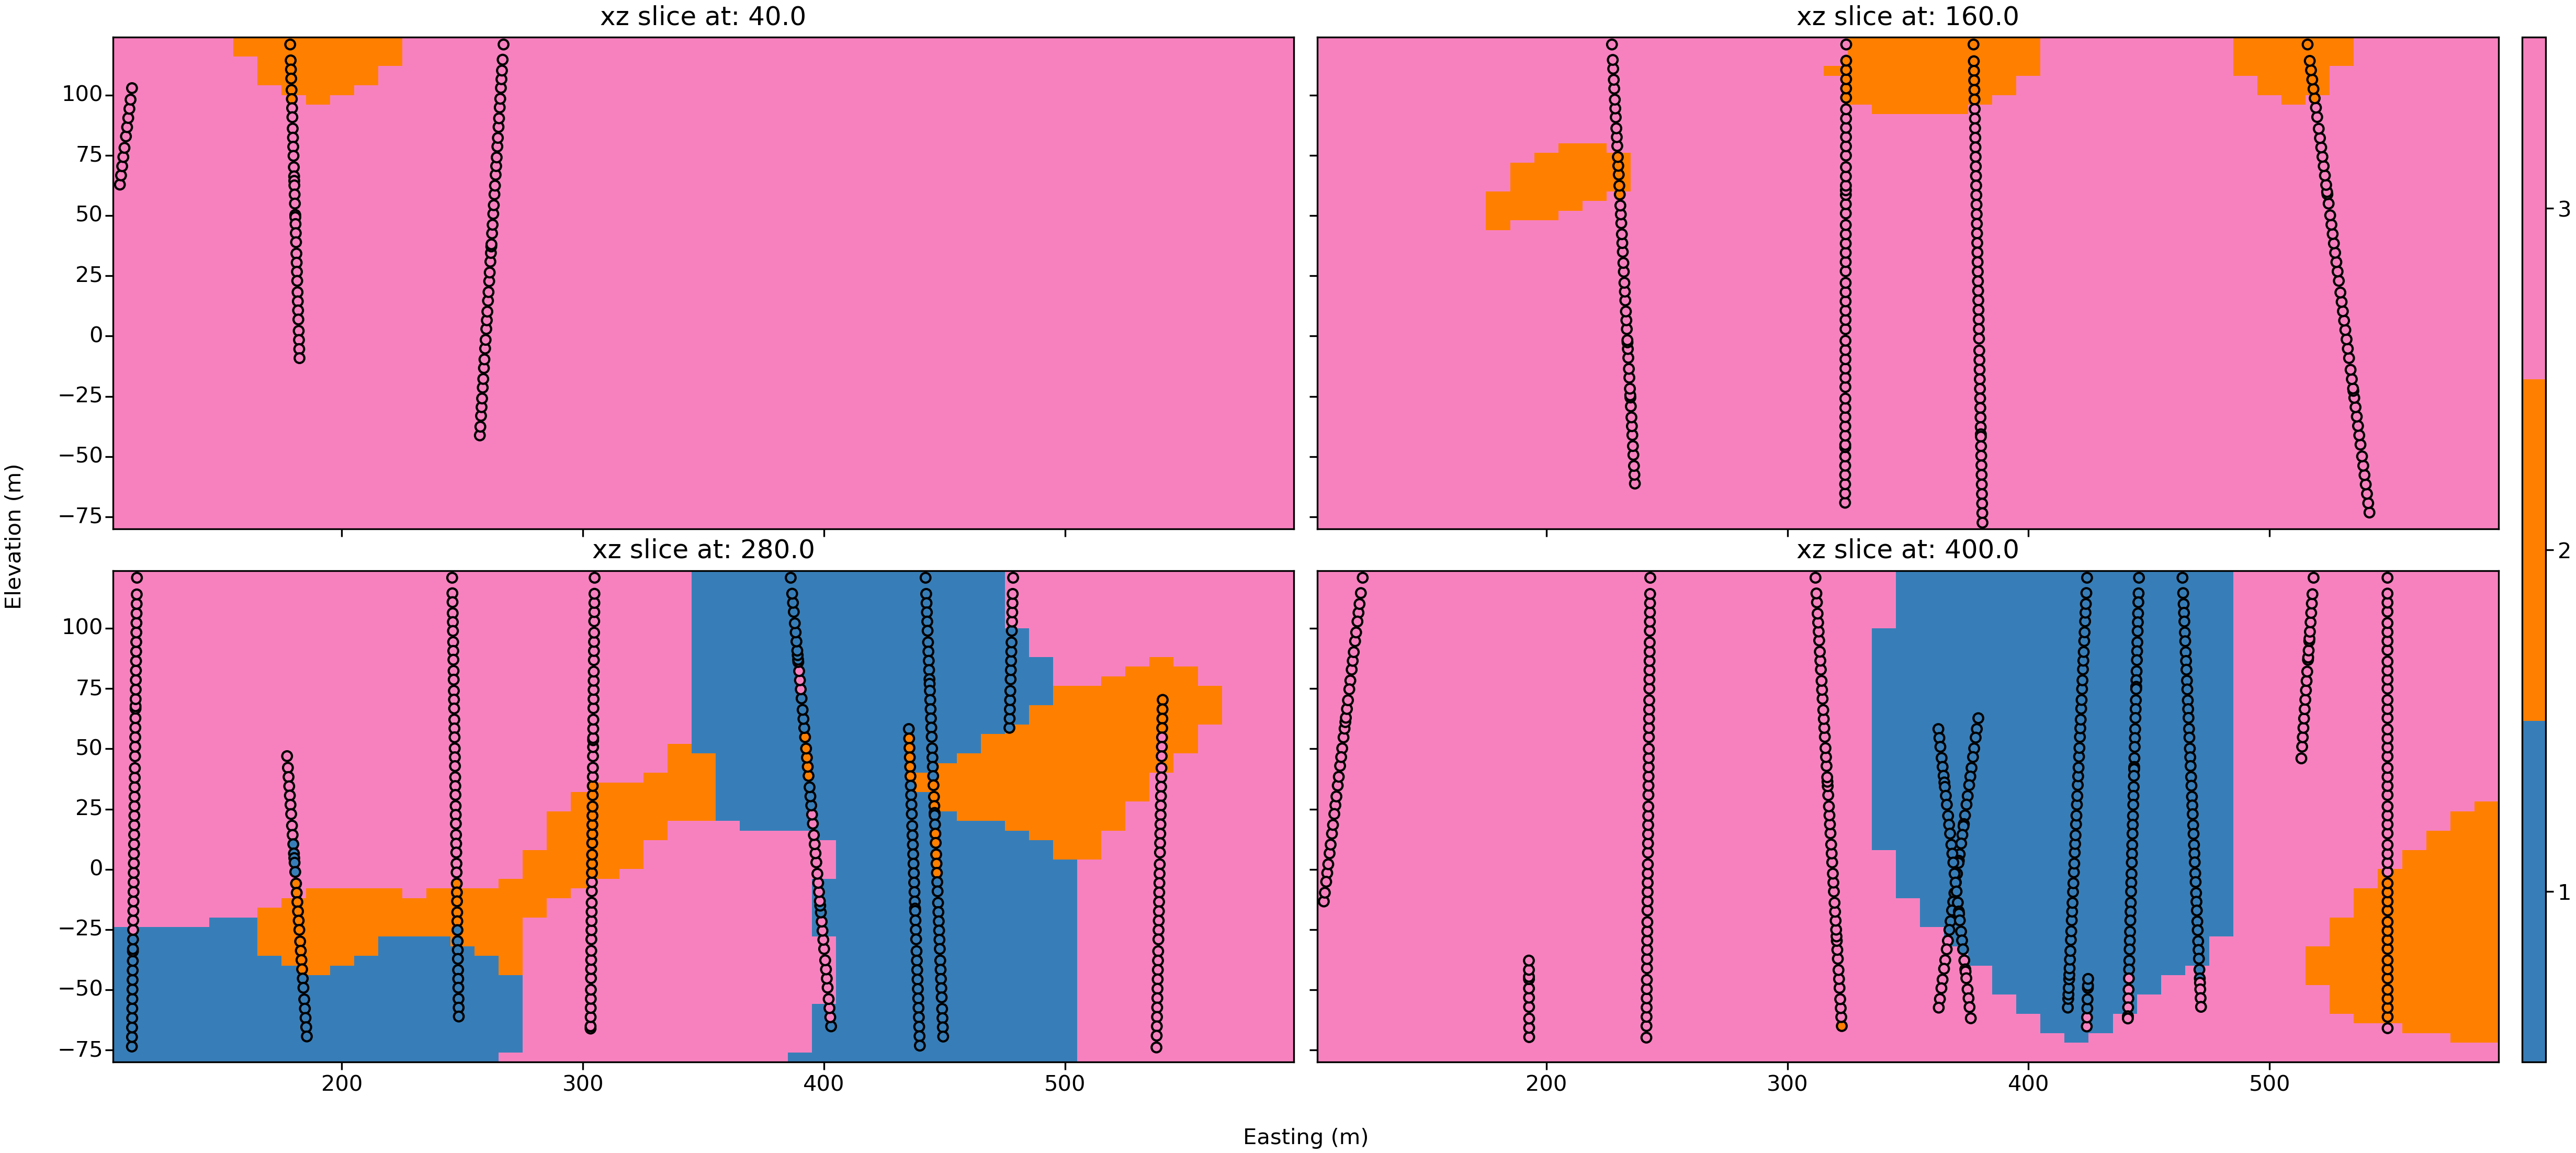
\includegraphics[width=0.8\textwidth]{capitulo_2/coarserxz.png}\label{a}}\\
\end{center}
\begin{center}
\subfloat[][Modelo geológico implícto no grid fino]{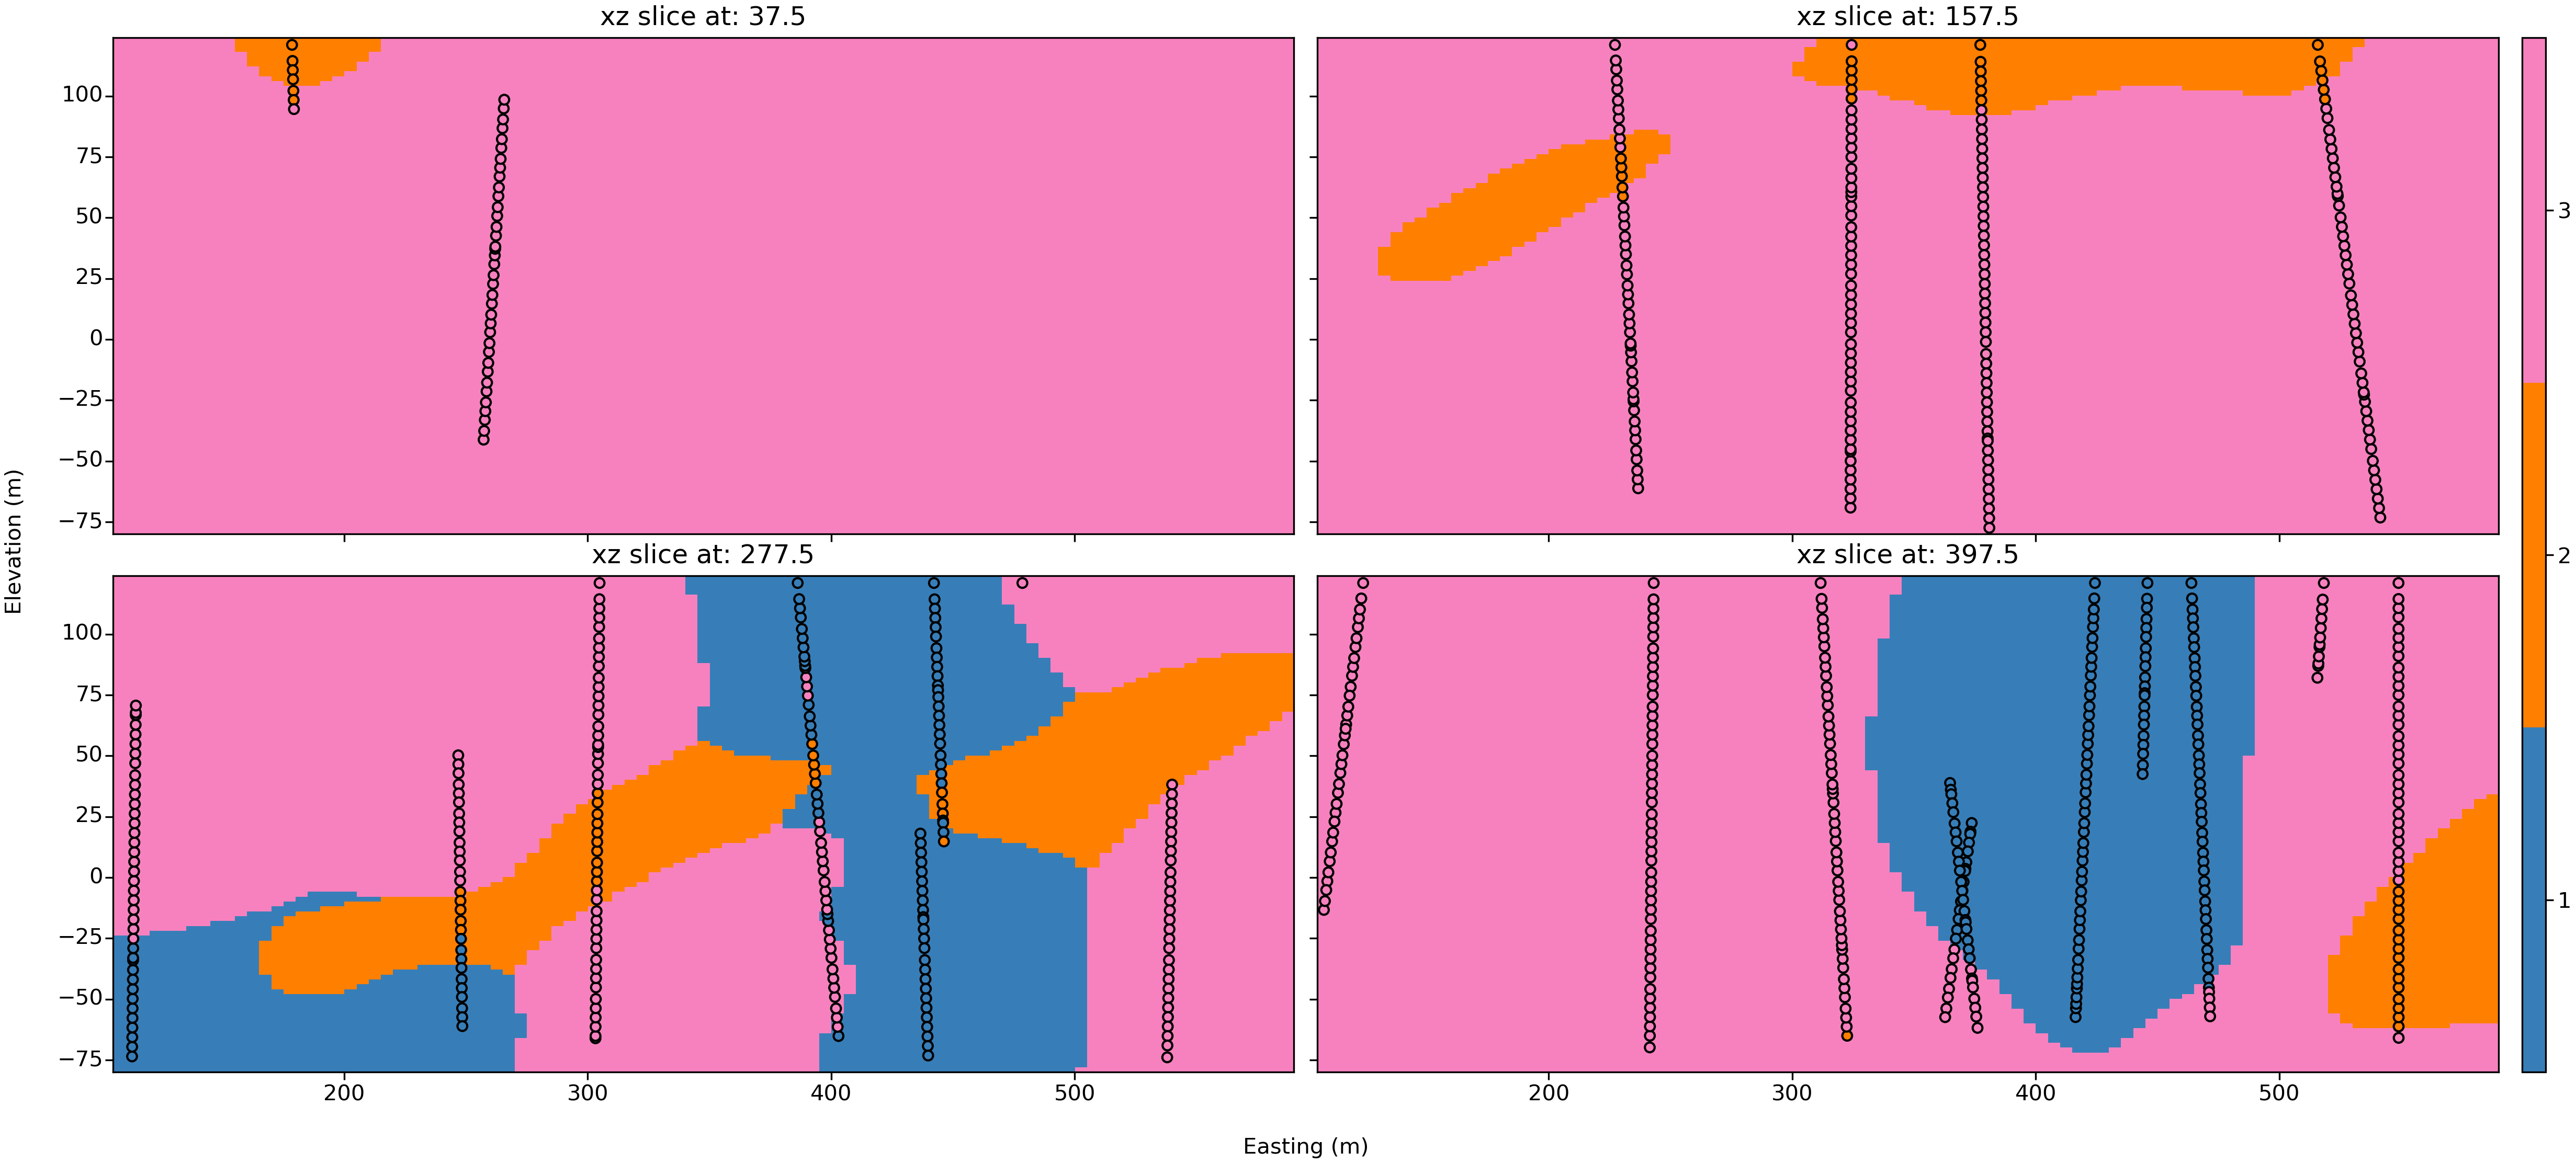
\includegraphics[width=0.8\textwidth]{capitulo_2/finerxz.png}\label{b}}
\end{center}
\end{figure}

\subsection{Métodos de interpolação}\label{met_int}

Qualquer método de interpolação pode ser utilizado, mesmo os métodos do inverso da distância produzem resultados realistas. A krigagem e as funções de bases radias permitem incorporar informação adicional através dos modelos de covariância parametrizados a partir das amostras e minimizam a variância do erro. A literatura recomenda uso de métodos globais, que usam todas as amostras para cada estimativa, para evitar o surgimento de artefatos nos modelos.

\citeonline{hosseini_deutsch_iqd} Utilizaram inverso da distância, \citeonline{silvaenhancedgeomodeling} utilizou krigagem ordinária global, \citeonline{rolo_dissertacao} utilizou krigagem ordinária, \citeonline{silva_dual} aplicou \textit{dual kriging} \citeonline{boisvert_geomodeling} gerou modelos implícitos através de distâncias assinaladas com anisotropia variável local (\textit{Locally varying anisotropy kriging - LVA}) e \citeonline{cowan2002rapid} propôs a utilização de interpoladores baseados em funções de bases radias (\textit{radial basis functions - RBF}), \citeonline{manchuck_MLS} ainda propuseram a utilização de mínimos quadrados móveis para incorporar interpretação manual e avaliar incerteza. A escolha do interpolador deve ser baseada em suas propriedades, na informação exigida para parametrizá-lo (o variograma, por exemplo) e nas sua capacidade de se ajustar a formas geológicas.

Especialmente para as funções distância assinaladas existe um problema adicional relacionado à estacionariedade, de primeira e segunda ordem. Existe uma forte tendência (\textit{trend}) que restringe os estimadores baseados em krigagem à krigagem ordinária para que a estacionairiedade seja mantida. Além disso, Formas geológicas são curvilíneas e não são bem descritas por funções de covariância lineares. Por esses motivos muitos autores preferem as funções de bases radiais já que ela não se baseia em estacionariedade de primeira ordem e honra localmente formas geológicas sem a necessidade de parametrização especial \cite{martin2017implicitmodeling}.

Independente do método de interpolação, os modelos gerados devem ser livres de artefatos para que os artefatos do modelo implícito não sejam transferidos para os modelos geológicos. Funções de bases radias e krigagem global garantem modelos livres de artefato por utilizarem todas as amostras em cada estimativa, já para os métodos baseados em inverso da distância e krigagem (não global) os parâmetros de busca são uma escolha crítica \cite{martin2017implicitmodeling}. No entanto, métodos globais possuem limitações em bancos de dados volumosos por dependerem de muito processamento e memória RAM.

A \autoref{interpo} mostra três modelos implícitos, para a categoria 1, interpolados por krigagem ordinária usando 40 amostras, krigagem ordinária usando 100 amostras e funções de bases radias, que é um método global. A krigagem ordinária global gerou modelos implícitos extremantes contínuos, mais do que o desejado, implicando em modelos geológicos não realistas. 

\begin{figure} 
    \caption{Interpolação das distâncias calculadas por diferentes métodos.} \label{interpo}
     \centering
     \subfloat[][OK com 40 amostras]{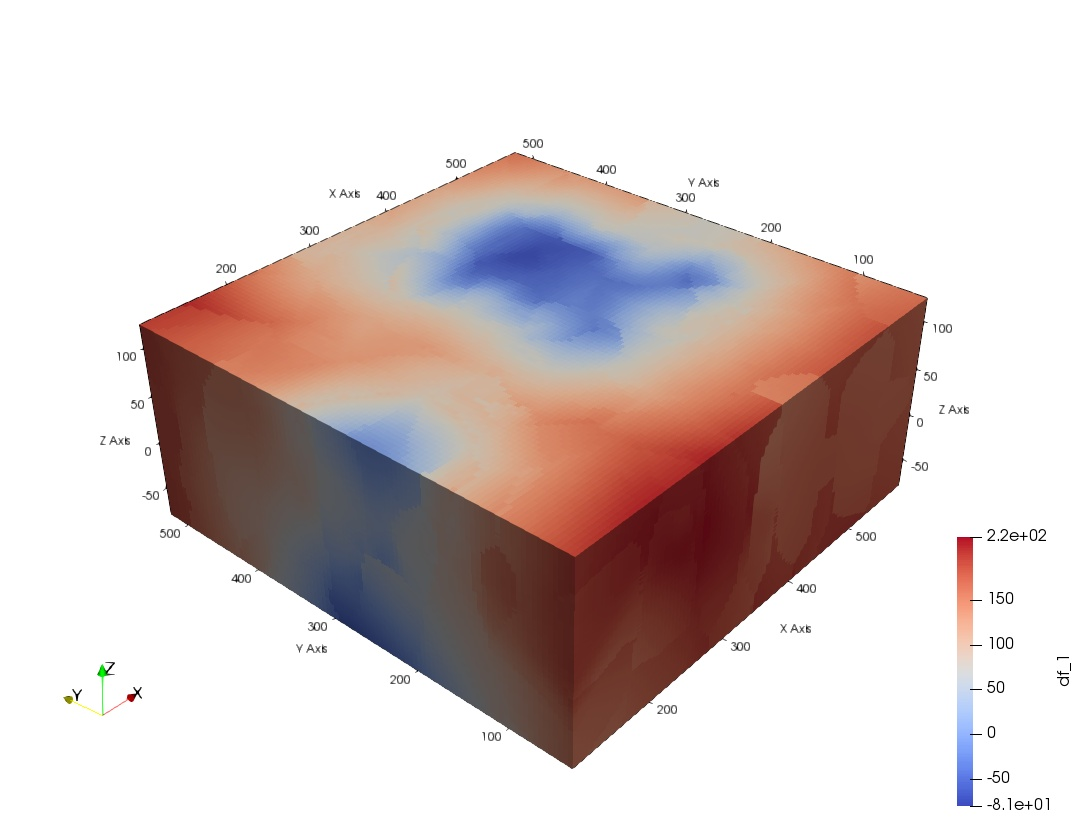
\includegraphics[width=.3\textwidth]{capitulo_2/kt3d40.jpeg}\label{<figure1>}}
     \subfloat[][OK com 100 amostras]{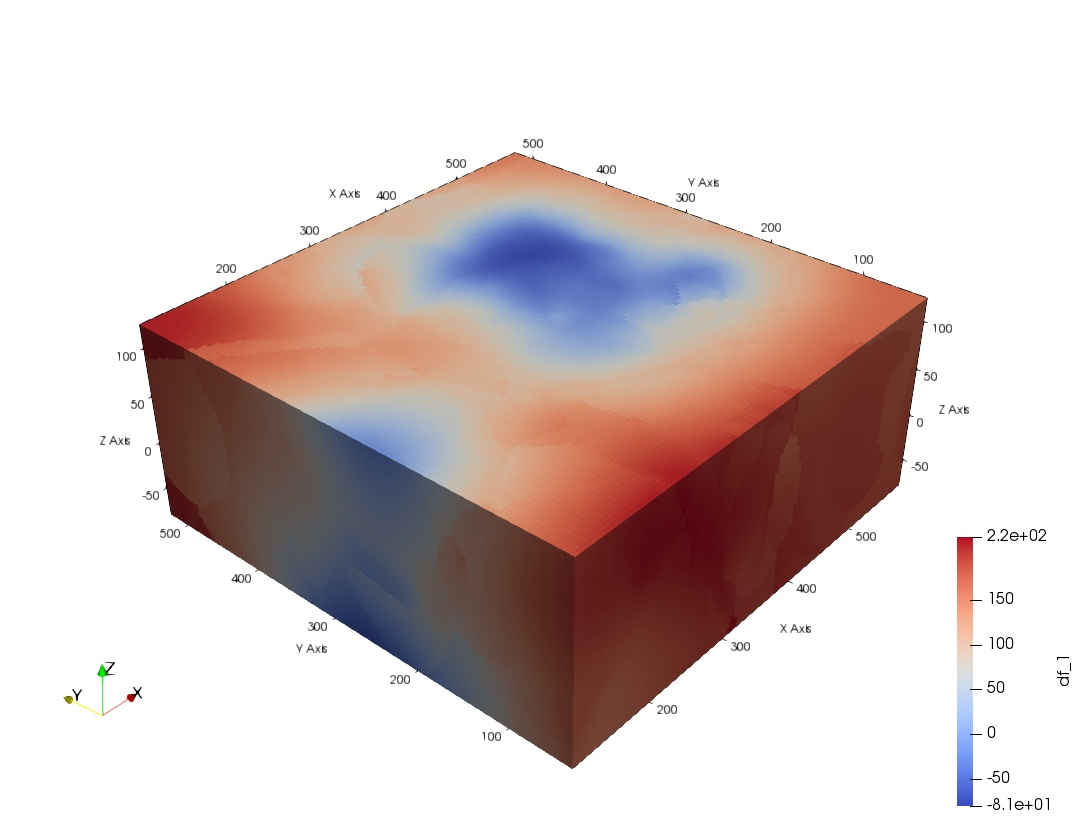
\includegraphics[width=.3\textwidth]{capitulo_2/kt3d100.jpeg}\label{<figure2>}}
     \subfloat[][RBF global]{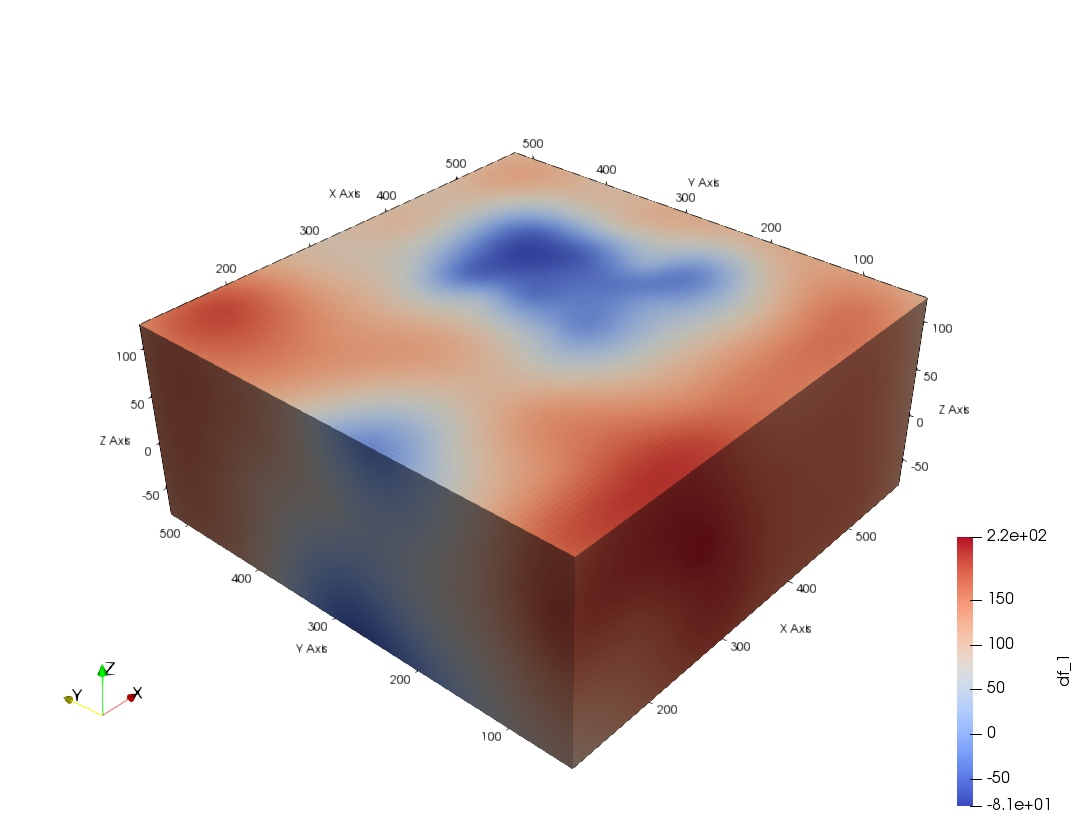
\includegraphics[width=.3\textwidth]{capitulo_2/rbf.jpeg}\label{<figure2>}}
\end{figure}

É evidente a presença de artefatos nos dois primeiros modelos. As funções de bases radiais criam um modelo suave e livre de artefatos. 

A \autoref{bench} mostra um \textit{Benchmark} dos diferentes métodos de interpolação. Todos os algoritmos utilizados são da biblioteca GSLib e foram executados em um core i7 7700HQ @ 2.8 GHz com 16 Gb de RAM.

O algoritmo de krigagem global não terminou de estimar os quase um milhão de blocos do grid fino sem terminar com uma mensagem de erro. A krigagem ordinária com 100 amostras leva 45 minutos contra pouco mais de um minuto do RBF, subdividindo o problema, é possível reduzir o tempo de interpolação para 16 segundos. Não é difícil perceber porque o RBF é o interpolador preferido na modelagem geológica implícita. O software comercial Leapfrog \textsuperscript{\textregistered} tem um algoritmo patenteado de RBF ainda mais rápido.

\begin{table}[]
\centering
\resizebox{\textwidth}{!}{%
\begin{tabular}{lllll}
Método & Tempo grid grosso & Tempo grid fino & Classificação errônea grosso & Classificação errônea fino \\ \hline
krigagem global isotrópica & 28min &  & 121 &  \\
krigagem global anisotrópica & 30min 34s &  & 282 &  \\
krigagem ordinária anisotrópica (40) & 1min 3s & 38min & 137 & 135 \\
krigagem ordinária anisotrópica (100) &  & 45min 51s &  & 181 \\
RBF isotrópico & 21.5s &  & 57 &  \\
RBF anisotrópico &  & 1min 22s &  & 38 \\
POU RBF anisotrópico &  & 1min 2s &  & 39 \\
POU RBF artefatos & 16.5s &  &  & 29 \\
LVA OK &  &  & 8 &  \\
LVA RBF &  &  &  & 8 \\
Krigagem dos indicadores &  & 33min 27s &  & 2 \\ \hline
\end{tabular}%
}
\caption{\textit{Benchmark} dos diferentes métodos de interpolação.} \label{bench}
\end{table}

\subsection{Funções de bases radiais - RBF}

A demonstração detalhada das equações e considerações  pode ser encontrada em \citeonline{martin_boisvert_review_rbf}. Os interpoladores baseados em funções de bases radiais são globais e não necessitam de um grid. Os pesos são treinados baseados nos valores da função distância assinalada calculados para cada ponto amostral. Com os pesos treinados o valor interpolado da função distância assinalada pode ser obtido rapidamente para qualquer localização do depósito. Esse procedimento permite treinar o sistema linear de equações antes de escolher o grid de interpolação \cite{martin2017implicitmodeling}.

\subsubsection{O \textit{kernel}}

O \textit{kernel} radial estabelece as relações espacias entre todos os pontos do domínio. O \textit{kernel} 
é sinônimo a função covariância usada na krigagem, e pode/deve ser parametrizado a partir do variograma, calculado e modelado a partir das amostras. Para modelagem geológica o \textit{kernel} Gaussiano, representado pela \autoref{gauss_kernel}, é o mais indicado. Na prática tanto o variograma das funções distância assinaladas: que são modelados com um pequeno efeito pepita (para evitar instabilidades matemáticas e/ou controlar o ruído do modelo) e estrutura Gaussiana, quanto o variograma dos indicadores: que é modelado com uma estrutura esférica \cite{martin2017implicitmodeling}, são adequados para a parametrização do \textit{kernel}. Os programas da biblioteca GSLib trabalham apenas com uma única estrutura. 

\begin{equation}\label{gauss_kernel}
  \phi(r)=exp^{-\epsilon^{-2}r^2}  
\end{equation}

Onde $\epsilon$ é o parâmetro de suporte, que defino o "range" do \textit{kernel}.

Para parametrizar as funções de bases radiais com o modelo de variograma (das distâncias ou indicadores) a distância de suporte do kernel pode ser estimada a partir do alcance na direção de maior continuidade do variograma análogo. Os ângulos e relações de anisotropia são parametrizados a partir da orientação e alcances dos variogramas análogos (azimuth, dip, rake, $r1 = \frac{a_{hmin}}{a_{hmax}}$, $r2 = \frac{a_{vert}}{a_{hmax}}$).

\citeonline{fasshauer2007meshfree} advoga que o \textit{kernel} pode ser parametrizado pela distância que representa a maior esfera que pode ser colocada entre amostras no domínio. Para modelagem geológica essa técnica tende a super estimar o suporte \cite{martin2017implicitmodeling}.

\subsubsection{Decomposição do domínio} \label{dom_decomp}

Como abordado na \autoref{met_int}: a limitação dos interpoladores globais são bancos de dados volumosos. Existem algumas técnicas para superar essa limitação como a solução iterativa \cite{beatson1999fast} por exemplo. Porém, um método que apresenta resultados satisfatórios e está presente na biblioteca GSLib é a decomposição do domínio (\textit{Partition of unity - POU}) \cite{wendland2004scattered}, que transforma um problema volumoso e que demanda muito esforço computacional em diversos problemas menores e eficientes que são, ao final, unidos.

A demonstração das equações e pode ser encontrada em \citeonline{wendland2004scattered} e \citeonline{martin_boisvert_review_rbf}. Um domínio $A$ é subdividido em uma série de partições sobrepostas $\beta$ de modo que a união de todas as $k$ partições em $A$, $\{ \beta \}^K_{j=1}$ compreende o domínio. Para cada partição, os dados correspondentes são utilizados interpolar a função escalar $s_j(x)$.

A função peso para cada partição deve ser igual a um no centro e 0 na fronteira, a contribuição de cada partição nos locais de sobreposição é dado pela função peso.

As partições são definidas encontrando uma série de coordenadas para os centros. Diversos métodos podem ser utilizados: um grid regular, k-means, árvore binária, \textit{oct tree}.

\begin{figure}[!htb]
	\caption{\label{pou}Particionamento.}
	\begin{center}
		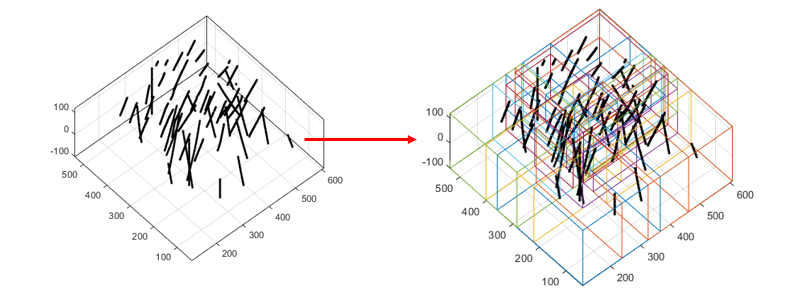
\includegraphics[width=0.7\textwidth]{capitulo_2/pou.jpg}
	\end{center}
	\legend{Fonte: \citeonline{martin_boisvert_review_rbf}}
\end{figure}

A \autoref{pou} mostra um domínio particionado: o particionamento começa considerando o domínio completo como sendo uma partição, então a partição "total" é subdividida recursivamente em duas mantendo um nível de sobreposição. O particionamento termina quando cada partição individual tem menos amostras que o máximo especificado pelo usuário \cite{martin2017implicitmodeling}. Dessa forma áreas com alta densidade amostral ficam em partições pequenas enquanto áreas esparsas ocupam partições maiores.

Deve haver um número de amostras em cada partição e sobreposição das partições suficientes para evitar o surgimento de artefatos quando as partições independentes forem unidas.

\section{Visualização do modelo geológico}

Como as funções distância são negativas no interior do domínio e positivas no exterior, um bom palpite inicial para a interface que separa os domínios no espaço, seria a linha (em duas dimensões) ou superfície (em três dimensões) que corresponda ao valor zero da função distância assinalada \cite{wildedeutschcalibrate}. 

A \autoref{isosup} mostra a iso superfície que representa a categoria 1, extraída no software Paraview, dos diferentes modelos implícitos da \autoref{interpo}. O algoritmo de extração de iso superfícies mais comumente utilizado é o dos cubos marchantes \cite{lorensen1987marching}. 

Note que os artefatos gerados nos modelos implícitos quando as distâncias foram interpoladas por krigagem são transferidos para as respectivas iso superfícies. Daí a importância de gerar modelos implícitos livres de artefatos.


\begin{figure} 
    \caption{Iso superfícies para a categoria 1 extraída dos diferentes modelos implícitos.} \label{isosup}
     \centering
     \subfloat[][OK com 40 amostras]{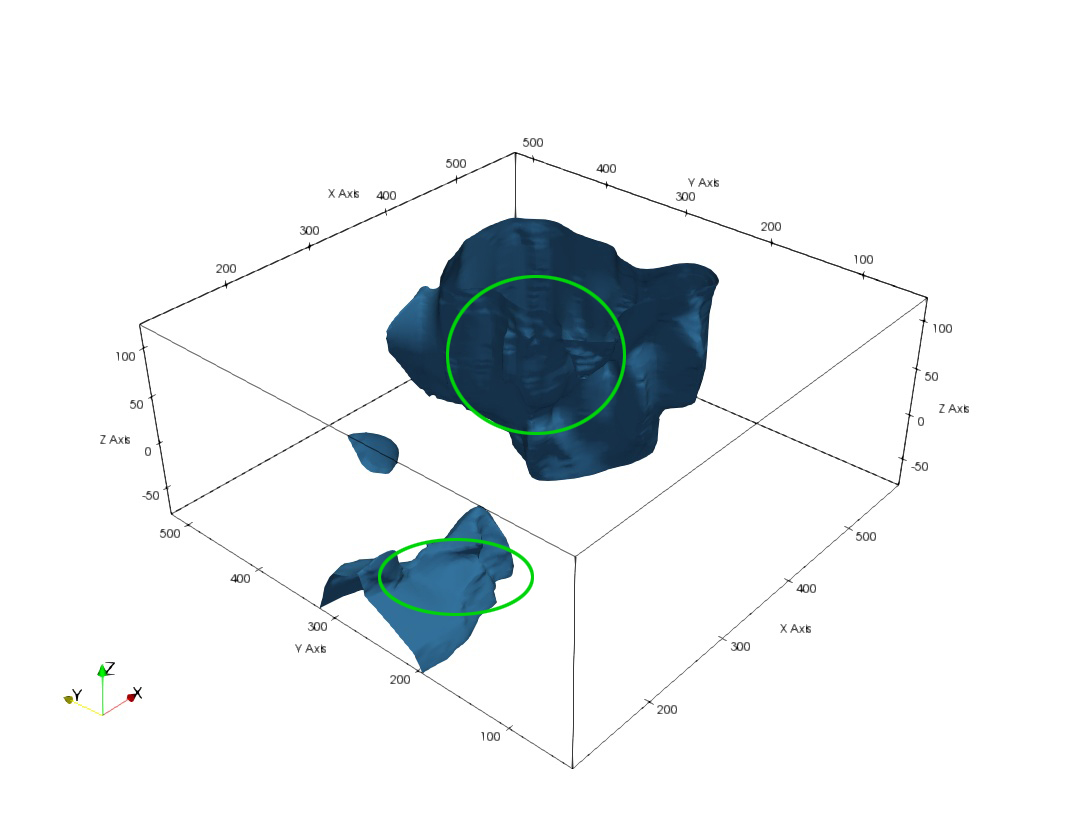
\includegraphics[width=.3\textwidth]{capitulo_2/isokt3d40.jpeg}\label{<figure1>}}
     \subfloat[][OK com 100 amostras]{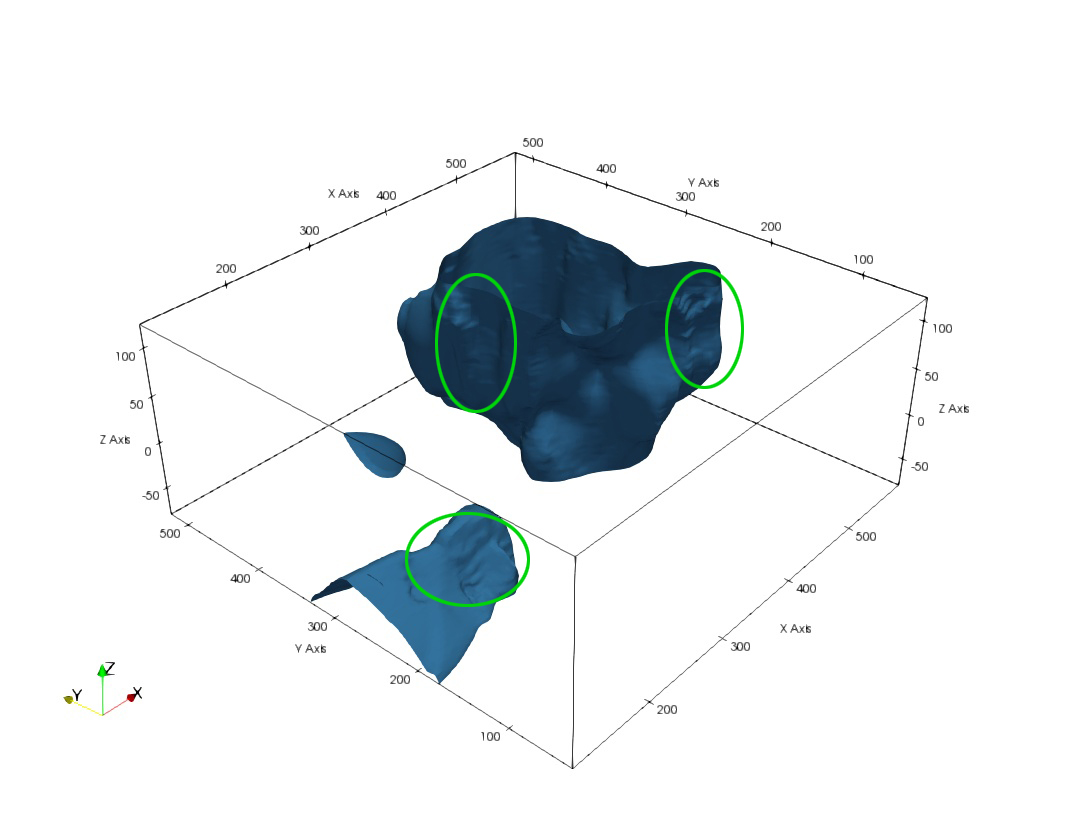
\includegraphics[width=.3\textwidth]{capitulo_2/isokt3dn100.jpeg}\label{<figure2>}}
     \subfloat[][RBF global]{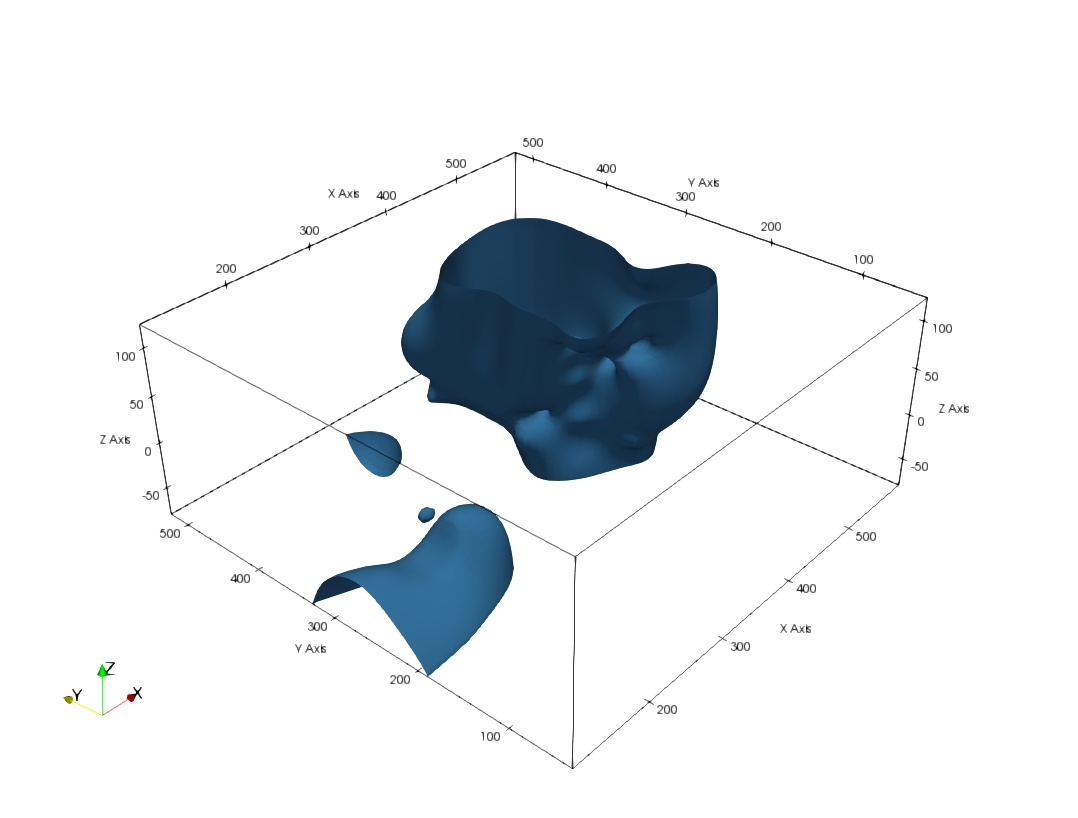
\includegraphics[width=.3\textwidth]{capitulo_2/isorbf.jpeg}\label{<figure2>}}
\end{figure}

Na presença de múltiplos domínios as iso superfícies devem ser extraídas uma a uma e algum tipo de regra hierárquica baseada na idade de cada litologia deve ser aplicada para a criação dos modelos multi categóricos.

As \autoref{iso_cat1} e \autoref{iso_cat2} mostram iso superfícies extraídas dos modelos implícitos interpolados por RBF e parametrizados a partir do variograma dos indicadores juntamente com as amostras categóricas no grid fino. 

\begin{figure} 
    \caption{Iso superfície extraída do modelo implícito interpolado por RBF para a categoria 1.} \label{iso_cat1}
     \centering
     \subfloat[][Vista 1]{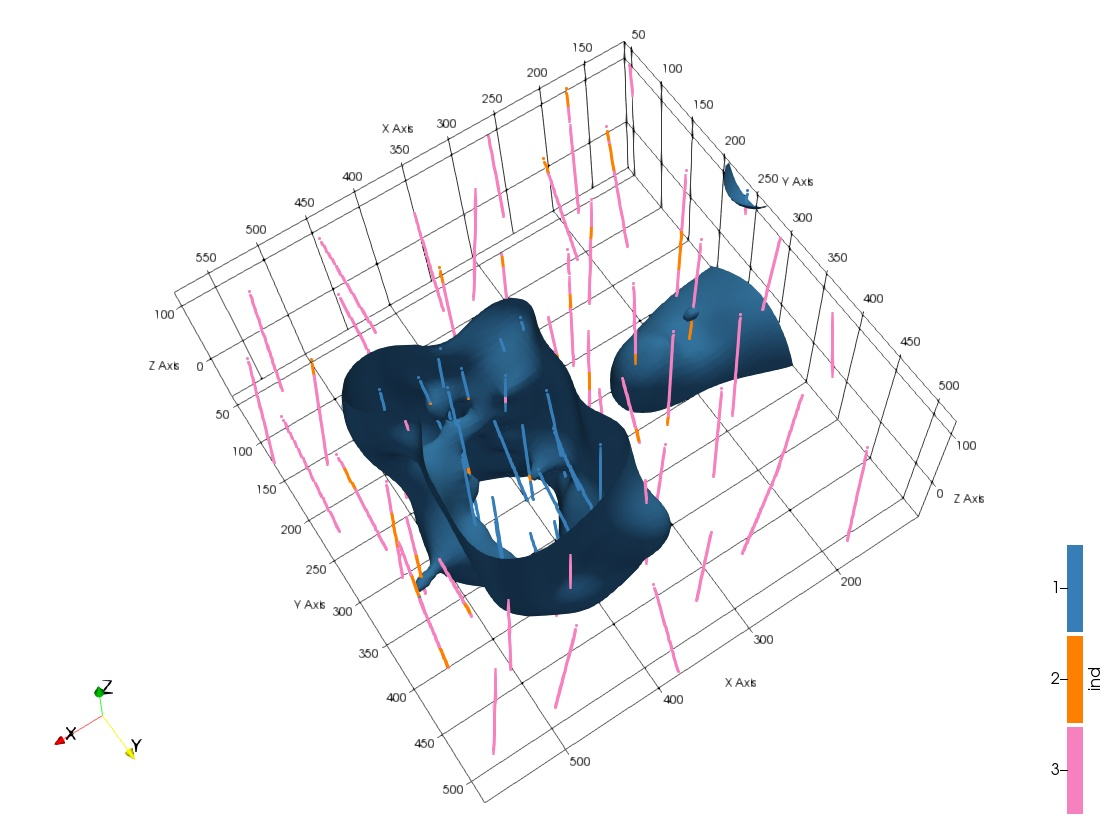
\includegraphics[width=.5\textwidth]{capitulo_2/iso_cat1_rbf.jpeg}\label{<figure1>}}
     \subfloat[][Vista 2]{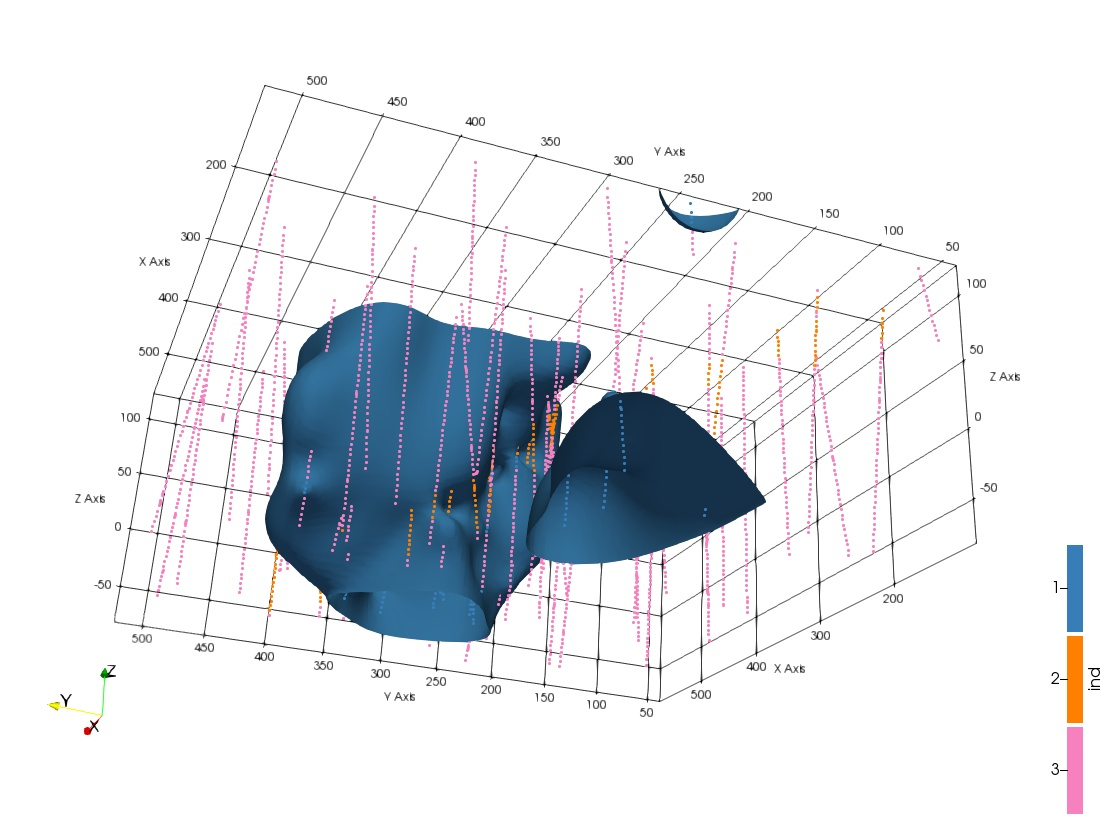
\includegraphics[width=.5\textwidth]{capitulo_2/iso_cat1_rbf2.jpeg}\label{<figure2>}}
\end{figure}

\begin{figure} 
    \caption{Iso superfície extraída do modelo implícito interpolado por RBF para a categoria 2.} \label{iso_cat2}
     \centering
     \subfloat[][Vista 1]{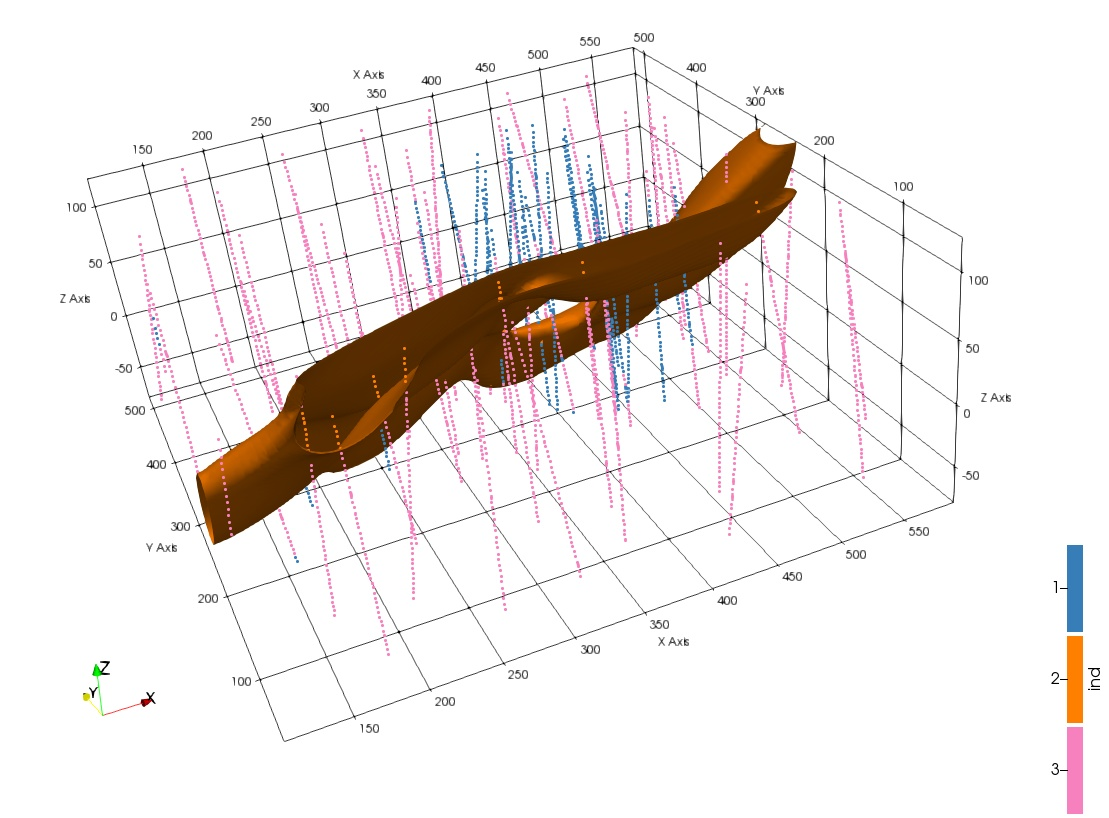
\includegraphics[width=.5\textwidth]{capitulo_2/iso_cat2_rbf.jpeg}\label{<figure1>}}
     \subfloat[][Vista 2]{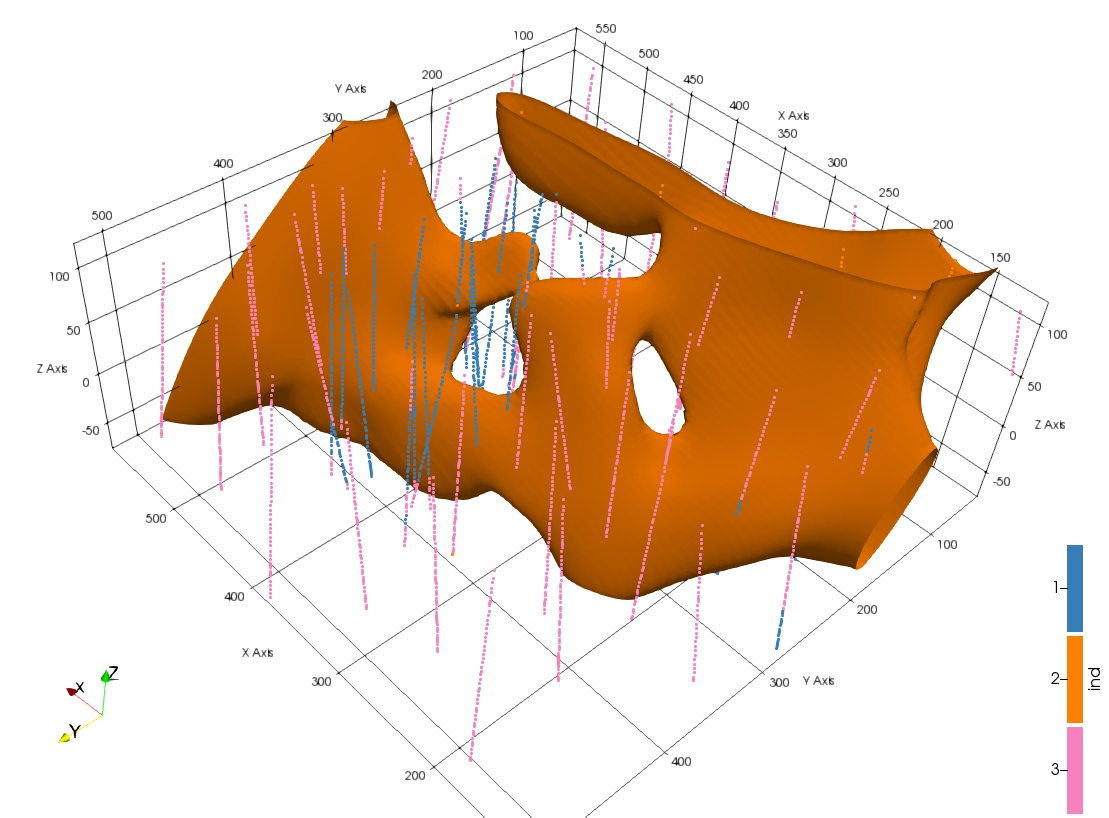
\includegraphics[width=.5\textwidth]{capitulo_2/iso_cat2_rbr2.jpeg}\label{<figure2>}}
\end{figure}

\subsection{Adaptação do método para múltiplas categorias simultâneas}\label{multi_cat}

\citeonline{silvaanddeutschccgmodeling} propuseram, uma adaptação para o método com o objetivo de modelar múltiplos domínios geológicos simultaneamente, de forma similar ao caso binário.

Se existirem $K$ múltiplos domínios no depósito mineral, para cada ponto amostral ${z(u_\alpha),\alpha=1,...,n}$, um vetor de indicadores de $K$ elementos é codificado de acordo com a \autoref{eq_mult_ind}.

\begin{equation}
	i_k(u_\alpha)=\begin{cases}
	1,\:\textrm{se}\:z(u_\alpha)=k\\
    0,\:\textrm{se}\:z(u_\alpha)\:\textrm{caso contrário}\end{cases} k=1,...,K
    \label{eq_mult_ind}
\end{equation}

A função distância é calculada, individualmente para cada elemento $k$ do vetor, de acordo com a \autoref{eq_mult_sg}.

\begin{equation}
	d_k(u_\alpha)=\begin{cases}
	-\parallel u_\alpha-u_\beta\parallel,\:\textrm{se}\:i_k(u_\alpha)=1\\
	+\parallel u_\alpha-u_\beta\parallel,\:\textrm{se}\:i_k(u_\alpha)=0\end{cases} k=1,...,K
    \label{eq_mult_sg}
\end{equation}

As distâncias calculadas são então interpoladas pelo método escolhido, individualmente para todos os nós do grid de acordo com a \autoref{eq_mult_ok}.

\begin{equation}
	d_k^*(u)=\sum\limits_{\alpha=1}^n \lambda_\alpha(u)d_k(u_\alpha)\quad k=1,...,K
    \label{eq_mult_ok}
\end{equation}

Por fim, cada bloco é  classificado pela \autoref{eq_mult_rt}

\begin{equation}
	i^*(u)=k'\;\text{de modo que}\;d_{k'}^*=min\{d_k^*(u)\}_{k=1}^K
    \label{eq_mult_rt}
\end{equation}

As distâncias estimadas fornecem uma medida de proximidade ao domínio oposto mais próximo. Sendo assim, a mínima distância assinalada estimada é tida como o domínio mais provável de ser encontrado numa região não amostrada. A \autoref{eq_mult_rt} sumariza essa ideia \cite{silvaenhancedgeomodeling}. A categoria associada com a menor distância estimada é retida em cada bloco.

A \autoref{mult_cat} mostra um exemplo de um modelo geológico criado a partir da mínima distância assinalada estimada. A esquerda, a figura mostra a projeção das distâncias assinaladas para cada uma das quatro categorias, e à direita a classificação final.

\begin{figure}[!ht]
    \caption{\label{mult_cat}Esquema para criação de um modelo implícito multi categórico.}
	\begin{center}
		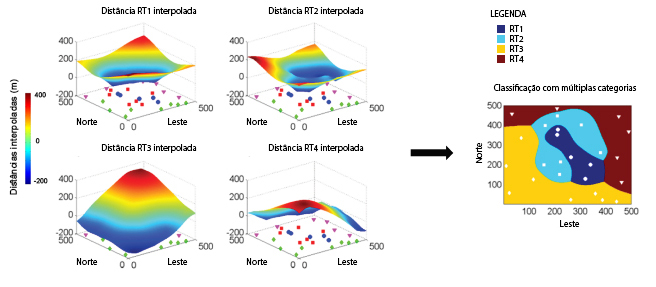
\includegraphics[width=0.8\textwidth]{capitulo_2/mult_cat_legenda.jpg}
	\end{center}
	\legend{Fonte: Modificado de \citeonline{silvageostatlessons}}
\end{figure}

A \autoref{multi_cat_rbf} mostra seções verticais em XZ e YZ de um modelo geológico implícito multi categórico criado por RBF parametrizado pelo variograma dos indicadores para o banco de dados do estudo de caso no grid fino. Nas seções também são mostradas amostras a 3 metros do centroide dos blocos na direção X e Y.

\begin{figure}[t]
\caption{Modelo geológico multi categórico} 
\label{multi_cat_rbf}
\begin{center}
\subfloat[][Seções em XZ do modelo implícito gerado por RBF no grid fino.]{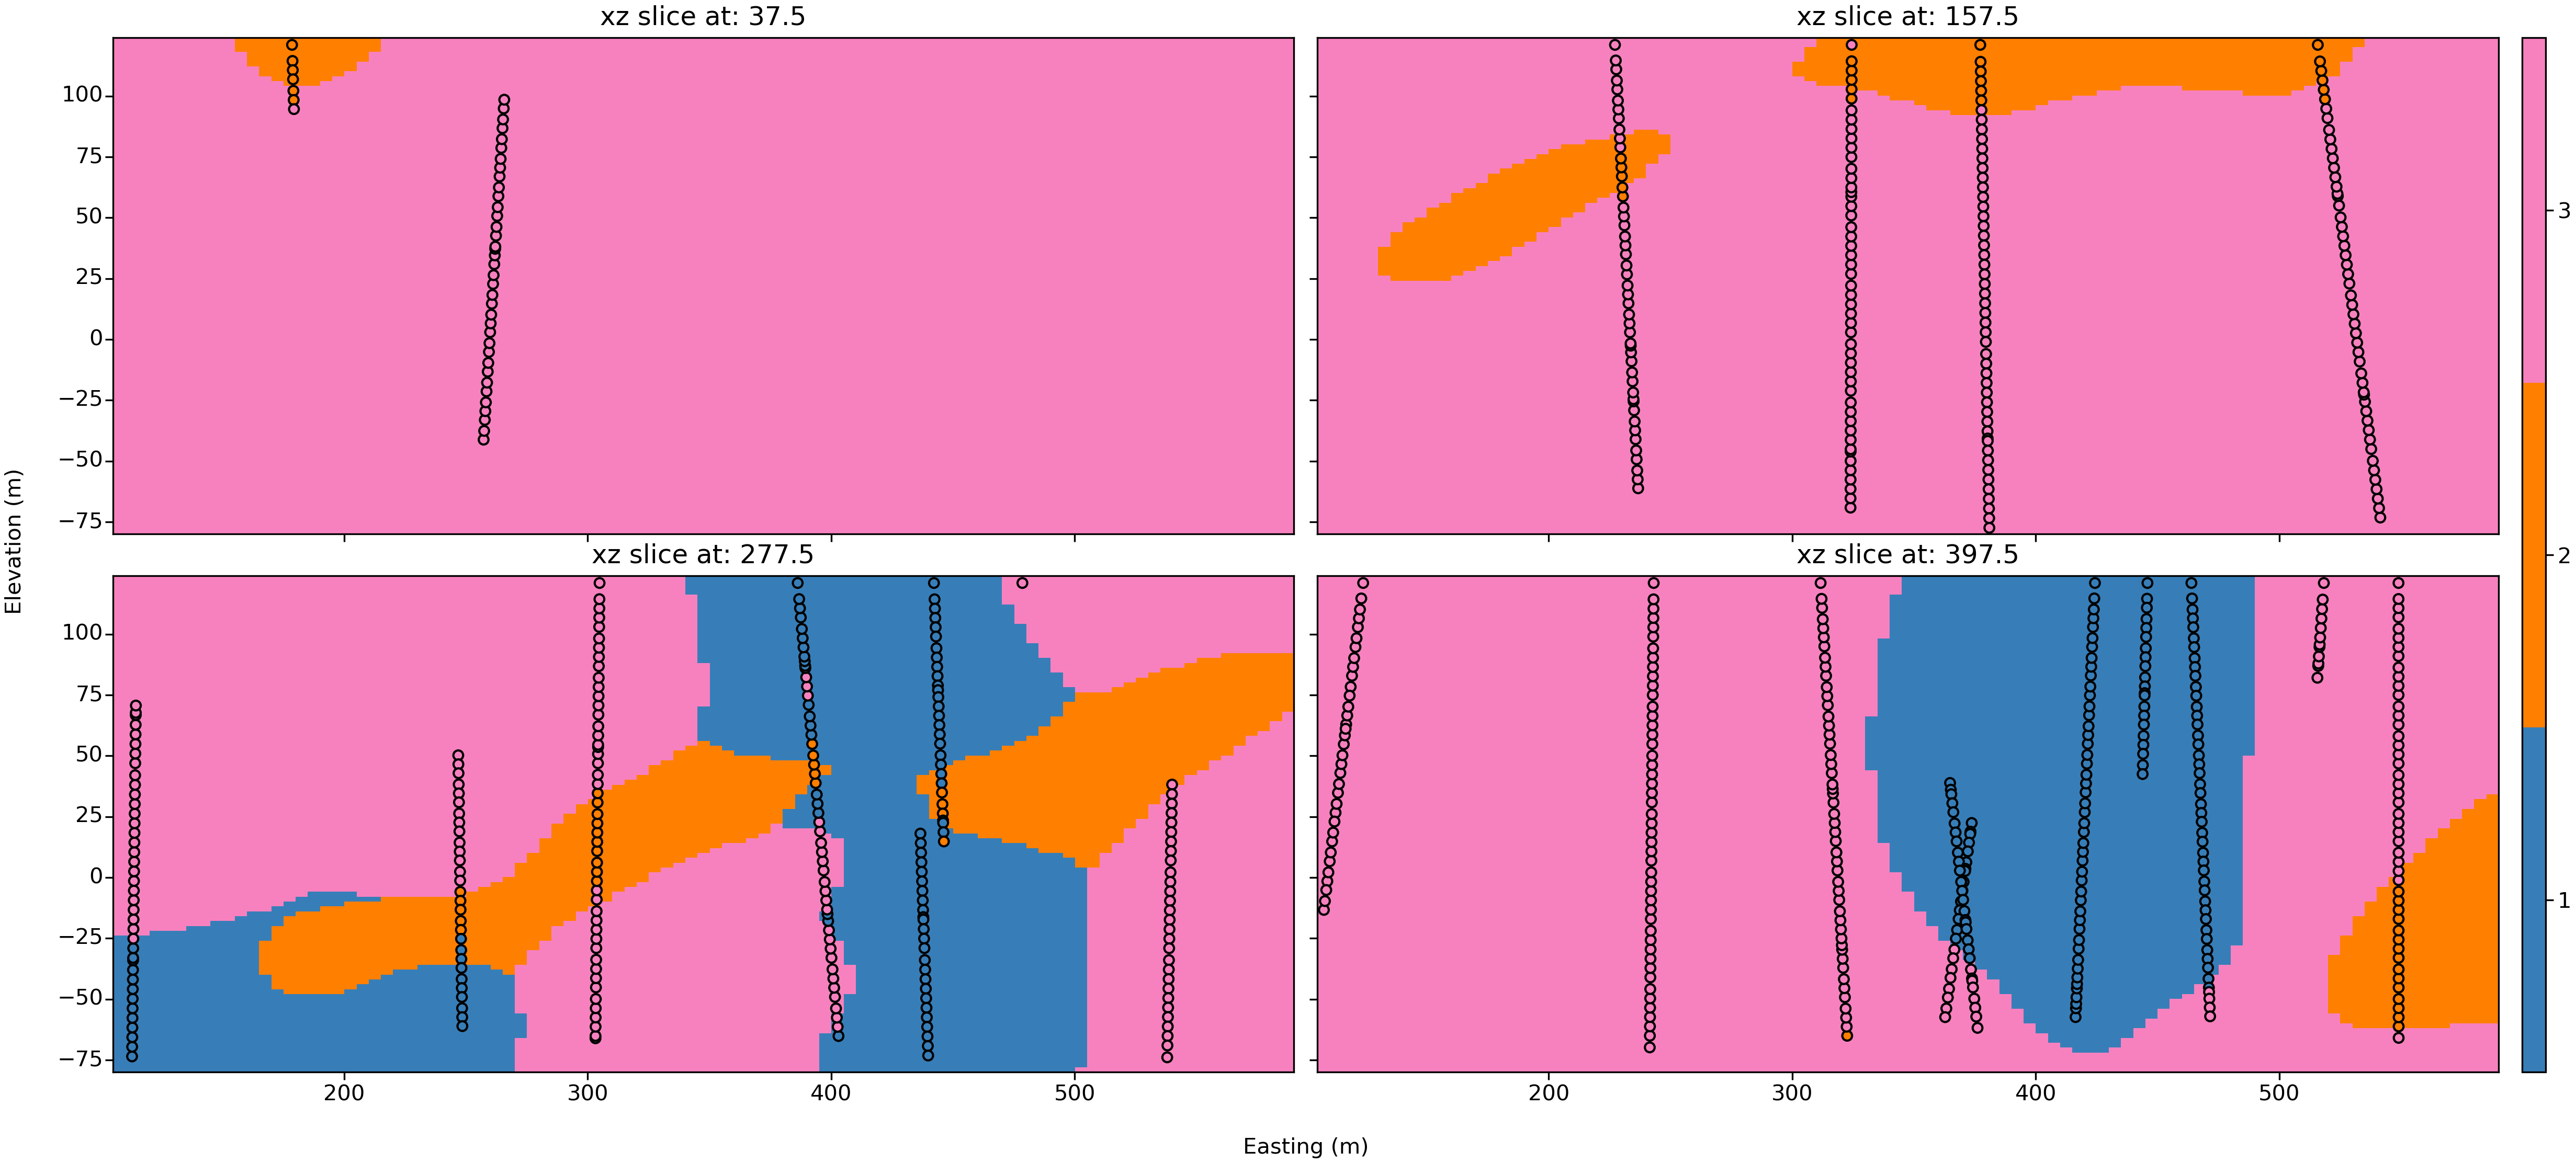
\includegraphics[width=0.8\textwidth]{capitulo_2/anisofinexz.png}\label{a}}\\
\end{center}
\begin{center}
\subfloat[][Seções em YZ do modelo implícito gerado por RBF no grid fino.]{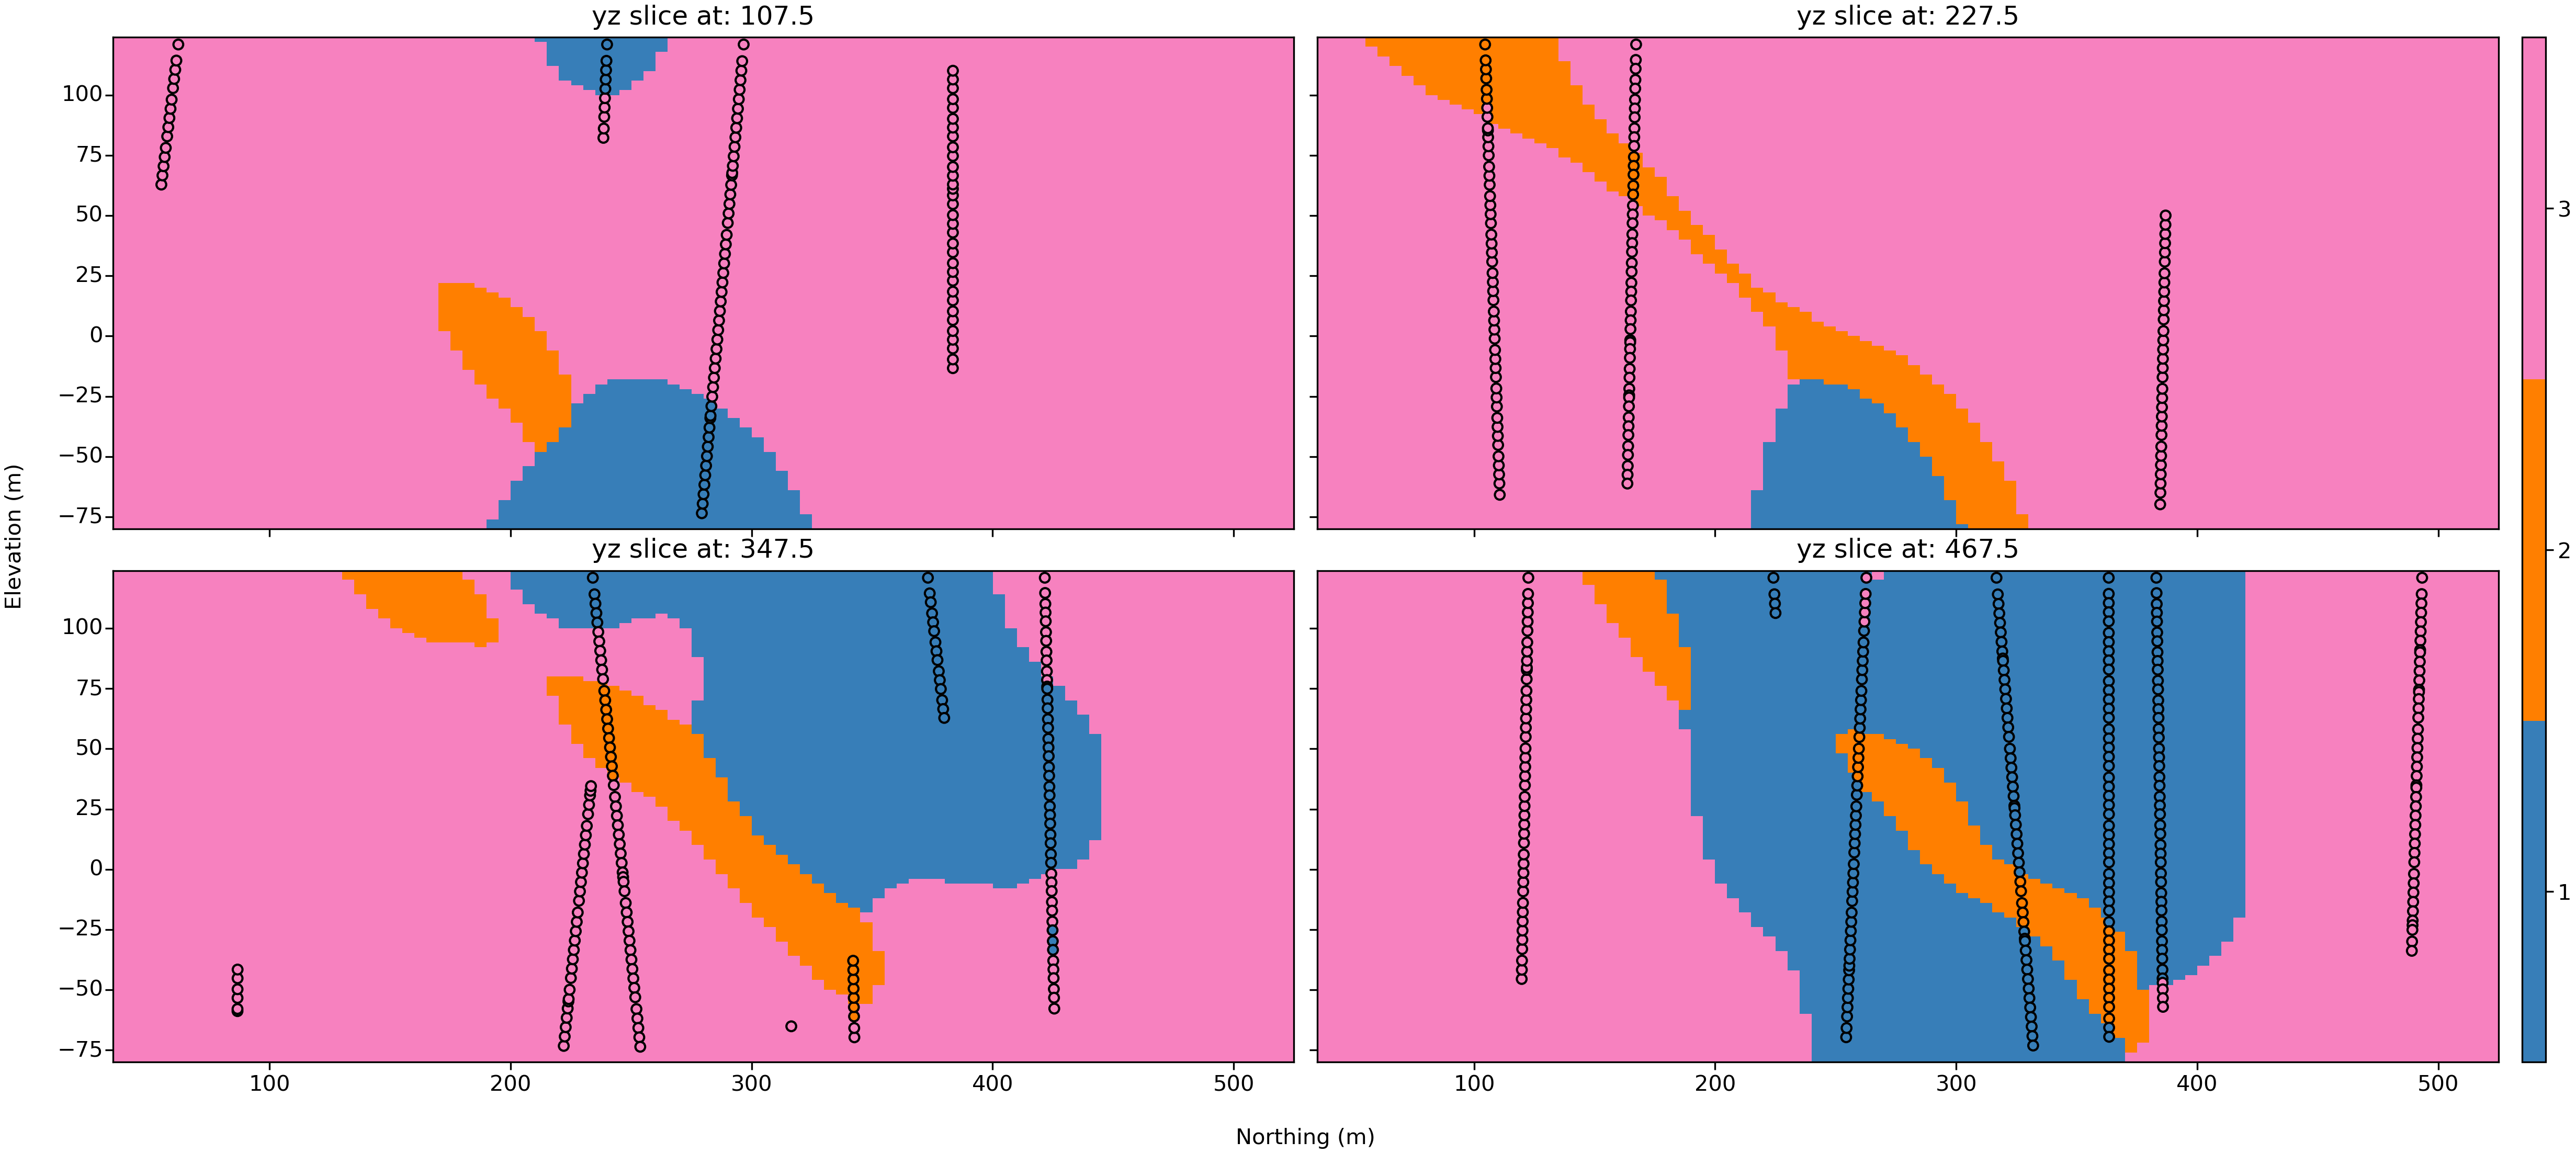
\includegraphics[width=0.8\textwidth]{capitulo_2/anisofineryz.png}\label{b}}
\end{center}
\end{figure}

A variação do método para múltiplos domínios ou categorias simultâneos deve ser utilizado com cautela, em muitos casos, em especial em depósitos com geologia complexa que apresentam intrusões, falhas e dobras é indicado a modelagem e análise das litologias individualmente, ou até mesmo com algum nível de interpretação geológica manual via digitalização de seções.

\section{Incorporação da não estacionariedade de segunda ordem}

Corpos geológicos são complexos da escala macro à escala micro. Essa característica pode tornar difícil a captura de suas feições com funções de covariância. Segundo \citeonline{martin2017implicitmodeling} a não estacionariedade de segunda ordem deve ser incorporada quando estruturas complexas estão sendo modeladas.

Anisotropia é definida como o conjunto de rotações e relações anisotrópicas: azimuth, dip, rake, $r1 = \frac{a_{hmin}}{a_{hmax}}$, $r2 = \frac{a_{vert}}{a_{hmax}}$. 

\subsection{Krigagem com anisotropia local variável}

A krigagem com anisotropia variável exige que os parâmetros locais de anisotropia sejam definidos em todos os nós do grid (\autoref{lva_krig_cartoon}), e variem de forma suave pelo domínio. Isso permite que estruturas curvilineares em escala menor que o espaçamento entre as amostras sejam capturadas \cite{martin2017implicitmodeling}. Porém, torna o método computacionalmente exigente.

\begin{figure}[!ht]
\caption{\label{lva_krig_cartoon}Esquema mostrando os vetores de anisotropia local para cada nó do grid.}
	\begin{center}
		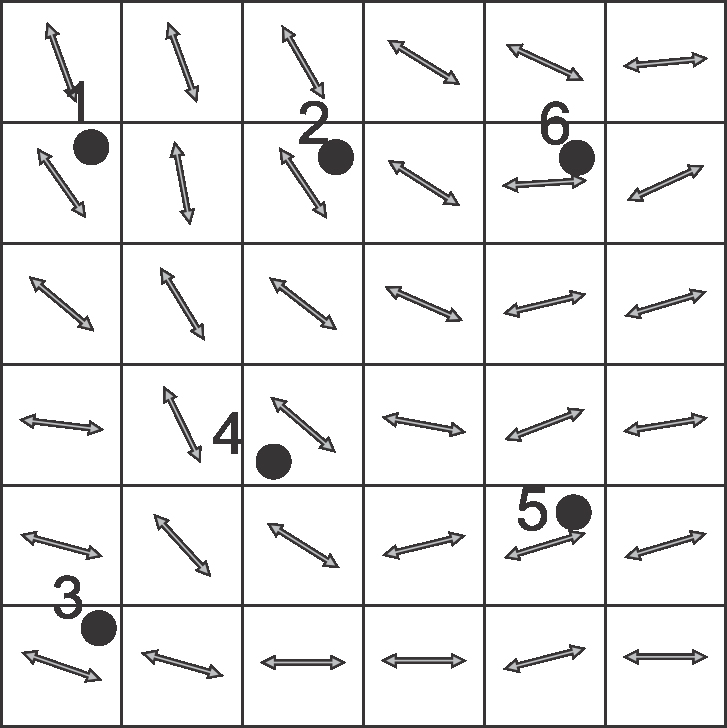
\includegraphics[width=0.3\textwidth]{capitulo_2/lvakrig.jpg}
	\end{center}
	\legend{Fonte: \citeonline{martin2017implicitmodeling}}
\end{figure}

Existem diversos métodos para definição da anisotropia local \cite{lillah2015inference}: pode ser inferida por um geomodelador, estimada diretamente a partir dos dados usando técnicas automáticas, interpolada de uma série de pontos onde a orientação foi medida ou pode ser extraída de dados em um grid que representam a variabilidade local (teores krigagdos, por exemplo). A bilioteca GSLib tem diversos softwares para definição de anisotropia local. 

A \autoref{lva_krig} mostra a iso superfície para a categoria 1 extraída de um modelo implícito gerado por krigagem com anisotropia local variável. Os vetores de anisotropia são plotados e foram gerados pelo software \verb|imorient| da biblioteca GSLib a partir de um modelo implícito para a categoria 1 previamente interpolado. A interpolação foi feita no grid grosso, a condição da anisotropia local para cada nó do grid torna o algoritmo computacionalmente exigente.

Esse programa analisa uma janela centrada em cada nó e estima a orientação dominante nessa janela, uma janela pequena captura variações em menor escala e uma janela grande variação de larga escala. É preciso encontrar um balanço \cite{lillah2015inference}.

\begin{figure} 
\caption{Iso superfície para a categoria 1 extraída de um modelo implícita gerado por krigagem com anisotropia local variável mostrando os vetores.} \label{lva_krig}
     \centering
     \subfloat[][Todos os vetores de anisotropia local]{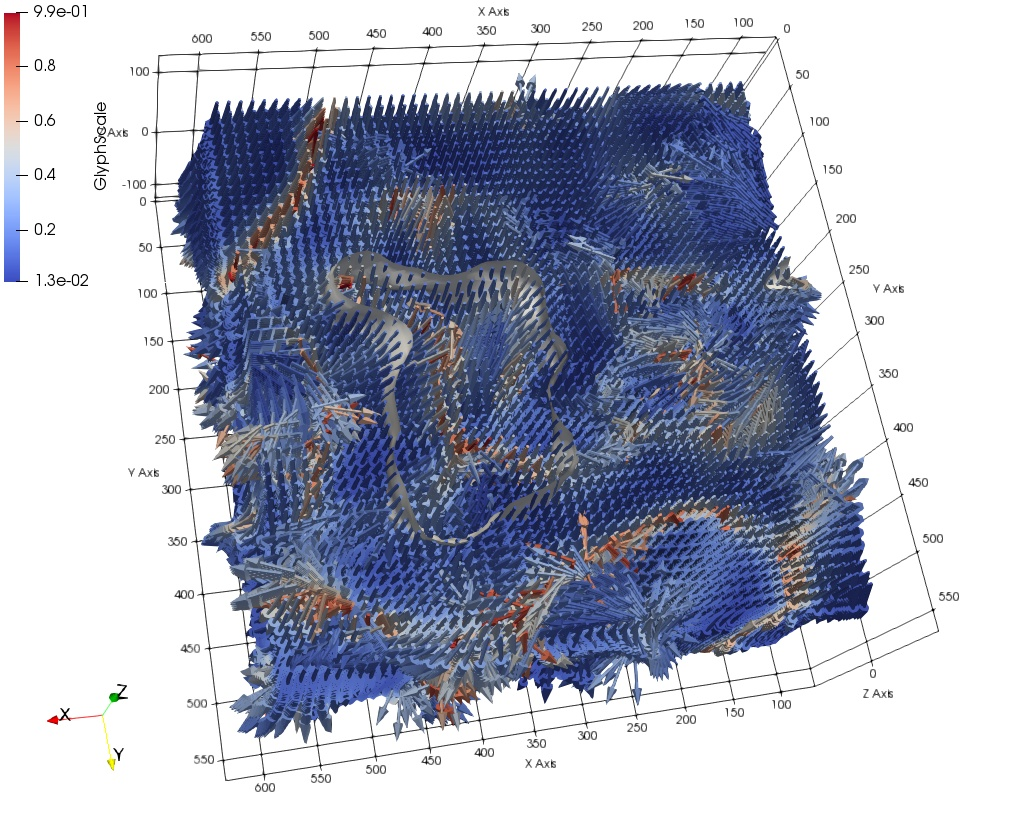
\includegraphics[width=.5\textwidth]{capitulo_2/lva_krig.jpeg}\label{<figure1>}}
     \subfloat[][Um vetor a cada 100.000 blocos]{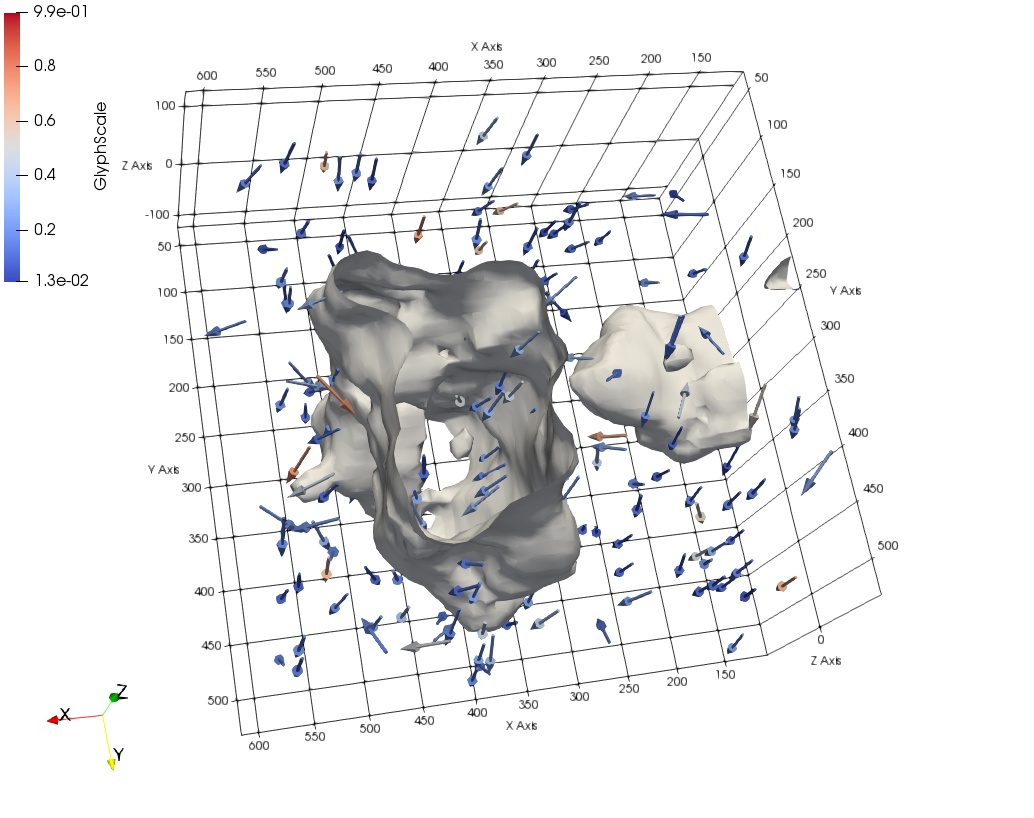
\includegraphics[width=.5\textwidth]{capitulo_2/lva_krig_100000.jpeg}\label{<figure2>}}
\end{figure}

\subsection{Funções de bases radias com anisotropia local variável}

RBF com anisotropia local variável é baseado na decomposição de domínios (\autoref{dom_decomp}), um kernel anisotrópico pode ser usado para melhor suportar os dados em cada partição, já que as partições são independentes uma matriz de rotação é usada para definir \textit{kernels} anisotrópicos locais que melhor se ajustam às propriedades espaciais de cada partição. O interpolador de bases radiais é obtido independentemente para cada partição e a solução final é obtida ponderando as soluções independentes nos locais de sobreposição \cite{martin2017implicitmodeling}.

Ao contrário da krigagem com anisotropia local variável, que requer os vetores de anisotropia em todas os nós do grid, a implementação para funções de bases radias requer os vetores somente no centro de cada partição (\autoref{lva_krig_cartoon}) e que variem suavemente pelo domínio.

\begin{figure}[!ht]
\caption{\label{lva_rbf+cartoon} Esquema mostrando os vetores de anisotropia local para cada centro de partição.}
	\begin{center}
		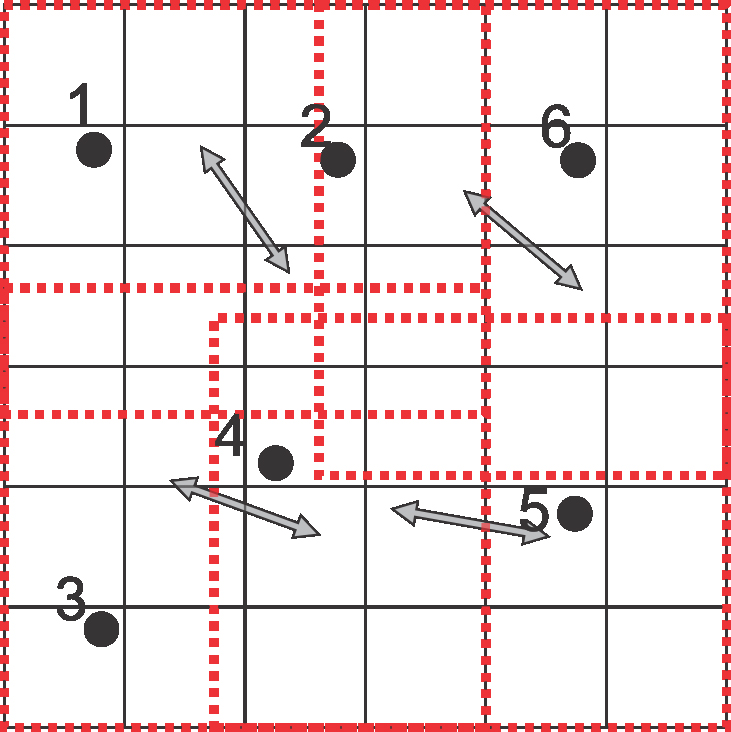
\includegraphics[width=0.3\textwidth]{capitulo_2/lvarbf.jpg}
	\end{center}
	\legend{Fonte: \citeonline{martin2017implicitmodeling}}
\end{figure}

A \autoref{rbf_iterref} mostra a iso superfície para a categoria 1 extraída de um modelo implícito gerado por funções de bases radiais com anisotropia local variável. Os vetores de anisotropia são plotados e foram gerados pelo software \verb|rbfiterref| da biblioteca GSLib. A interpolação foi feita no grid fino.

\begin{figure}[!ht]
\caption{\label{rbf_iterref}Iso superfície para a categoria 1 extraída de um modelo implícita gerado por krigagem com anisotropia local variável mostrando os vetores.}
	\begin{center}
		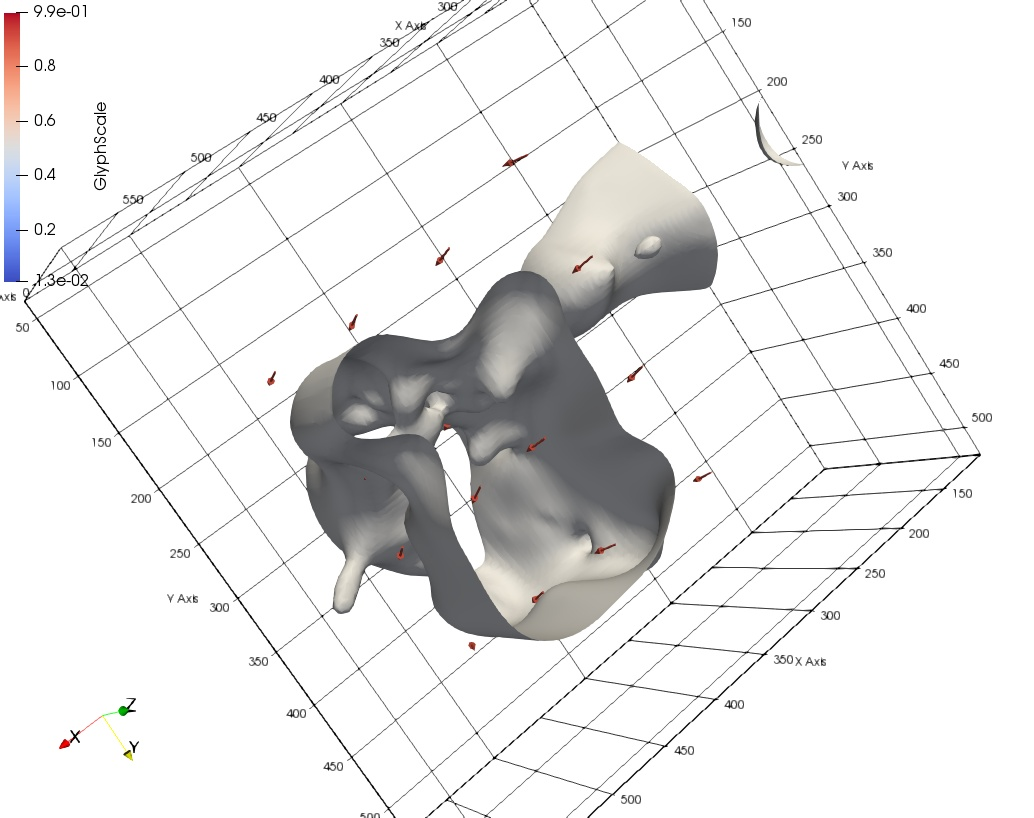
\includegraphics[width=0.5\textwidth]{capitulo_2/rbf_iterref.jpeg}
	\end{center}
	%\legend{Fonte: Modificado de \citeonline{silvageostatlessons}}
\end{figure}

\subsection{Refinamento iterativo}

Extrair orientações locais de um modelo criado com anisotropia global e utilizar essas orientações em uma nova interpolação não estacionária resulta em um modelo geológico mais refinado considerando informação local. Esse processo pode ser repetido, continuamente refinando o campo de anisotropias locais. 

O refinamento iterativo com funções de bases radias tem um benefício extra (em relação à krigagem com variação local de anisotropia), a possibilidade de incluir algum tipo de critério de parada, quando o modelo for considerado refinado. Como as partições são independentes, se o refinamento de uma partição em particular não resultará em mudanças significativas, pode ser omitido na solução final. Essa característica torna o processo significativamente mais rápido \cite{martin2017implicitmodeling}.

A \autoref{iterref} mostra um processo de refinamento iterativo onde a semente é um modelo isotrópico. O programa \verb|rbfiterref| começa sua execução inferindo orientações anisotrópicas em cada flanco da dobra, que são rasos demais para que sejam definidos adequadamente. Porém, nas próximas iterações do refinamento o mergulho se torna mais profundo e os flancos são definidos implicitamente.

\begin{figure}[!ht]
\caption{\label{iterref} Esquema mostrando o refinamento iterativo para funções de bases radiais.}
	\begin{center}
		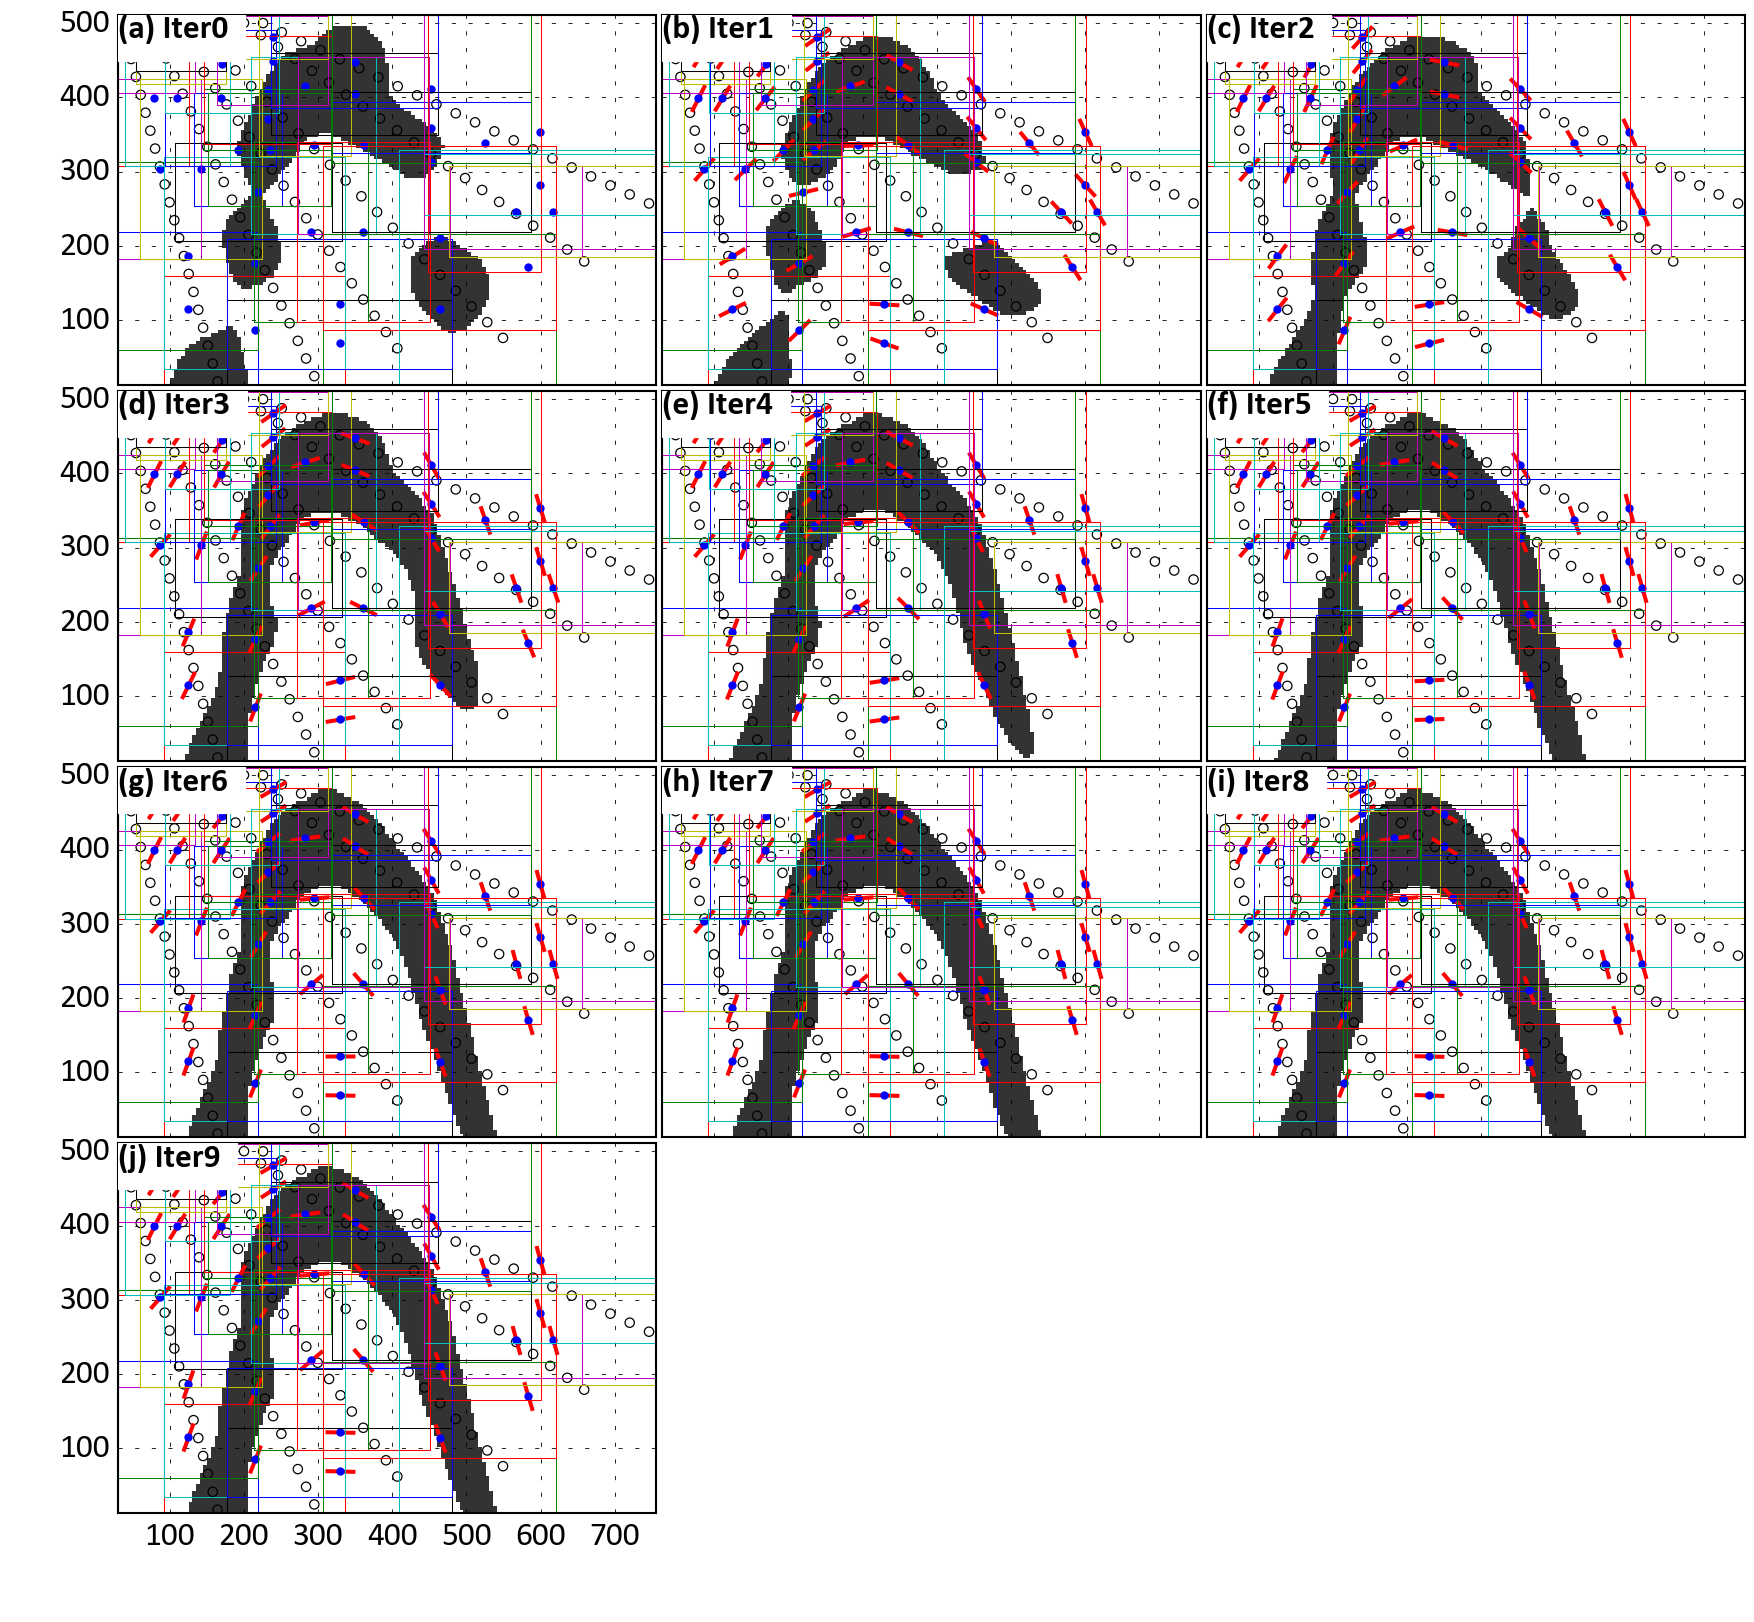
\includegraphics[width=0.7\textwidth]{capitulo_2/iterref.jpg}
	\end{center}
	\legend{Fonte: \citeonline{martin2017implicitmodeling}}
\end{figure}

\section{Incorporação de informação secundária}

Modelos explícitos englobam julgamento profissional que é difícil de superar por qualquer
algoritmo implícito devido à complexidade de representar objetos naturais com funções numéricas, principalmente quando os dados são esparsos. 

Uma desvantagem da modelagem implícita é que muitas vezes o modelo resultante não está de acordo com a interpretação e expectativa do geomodelador. Assistência humana usualmente é necessária para construir modelos geológicos semi automáticos utilizando técnicas que utilizem informação explícita e implícita  como a interpolação suave discreta (\textit{Discrete smooth interpolation - DSI}) \cite{malletgeomodeling}. Nas primeiras fases da mineração a proporção explícita da modelagem é maior, a medida que mais dados são obtidos, a proporção de intervenção humana é menor \cite{manchuck_MLS}.

O uso da krigagem ou funções de bases radiais limita os dados ao suporte puntual. \citeonline{manchuck_MLS} propõe o uso de uma regressão linear local chamada mínimos quadrados móveis (\textit{Moving least squares - MLS}) que ajusta uma função aos dados para integrar modelagem geológica implícita e explicita. MLS é um algoritmo de interpolação geral que pode ser usado para ajustar uma função em pontos, linhas e polígonos. 
MLS foi escolhido por sua capacidade de interpolar dados em linha de forma exata. Representar as linhas como pontos discretos ou utilização de integração numérica não é necessário. 

\citeonline{manchuck_MLS} conduziram um estudo de caso em um banco de dados real de ouro, o banco de dados e o resultado final podem ser vistos na \autoref{mls_model}.

\begin{figure}[t]
\caption{Modelo geológico híbrido criado a partir de furos de sondagem e seções interpretadas.}\label{mls_model}
\begin{center}
\subfloat[][Seção mostrando furos e seções interpretadas.]{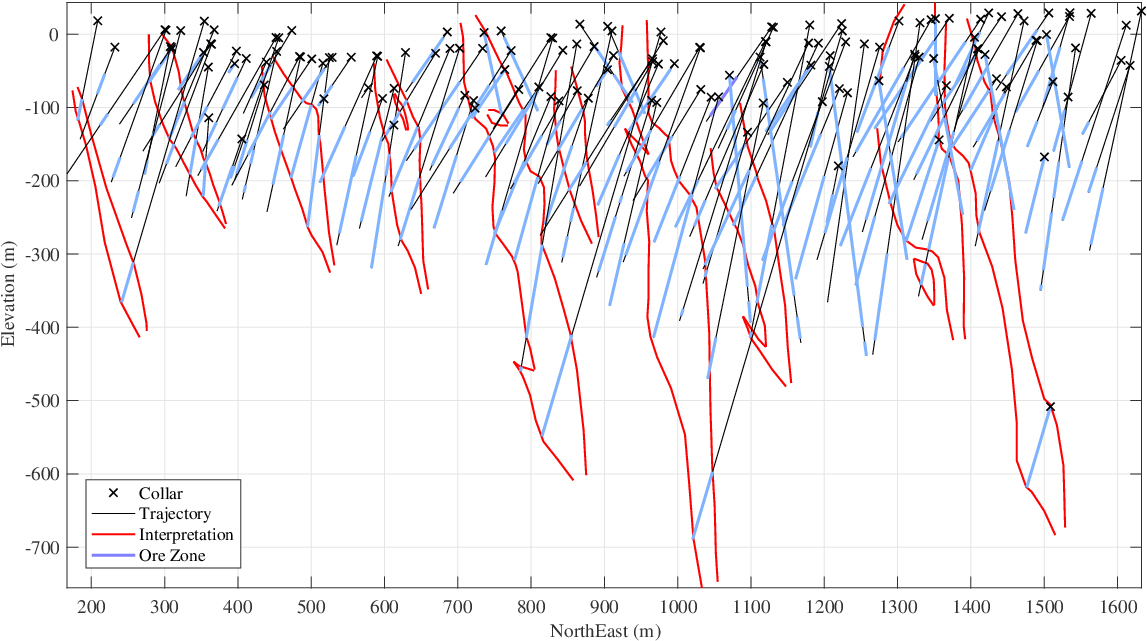
\includegraphics[width=0.8\textwidth]{capitulo_2/secoes.jpg}\label{a}}\\
\end{center}
\begin{center}
\subfloat[][Modelo implícito.]{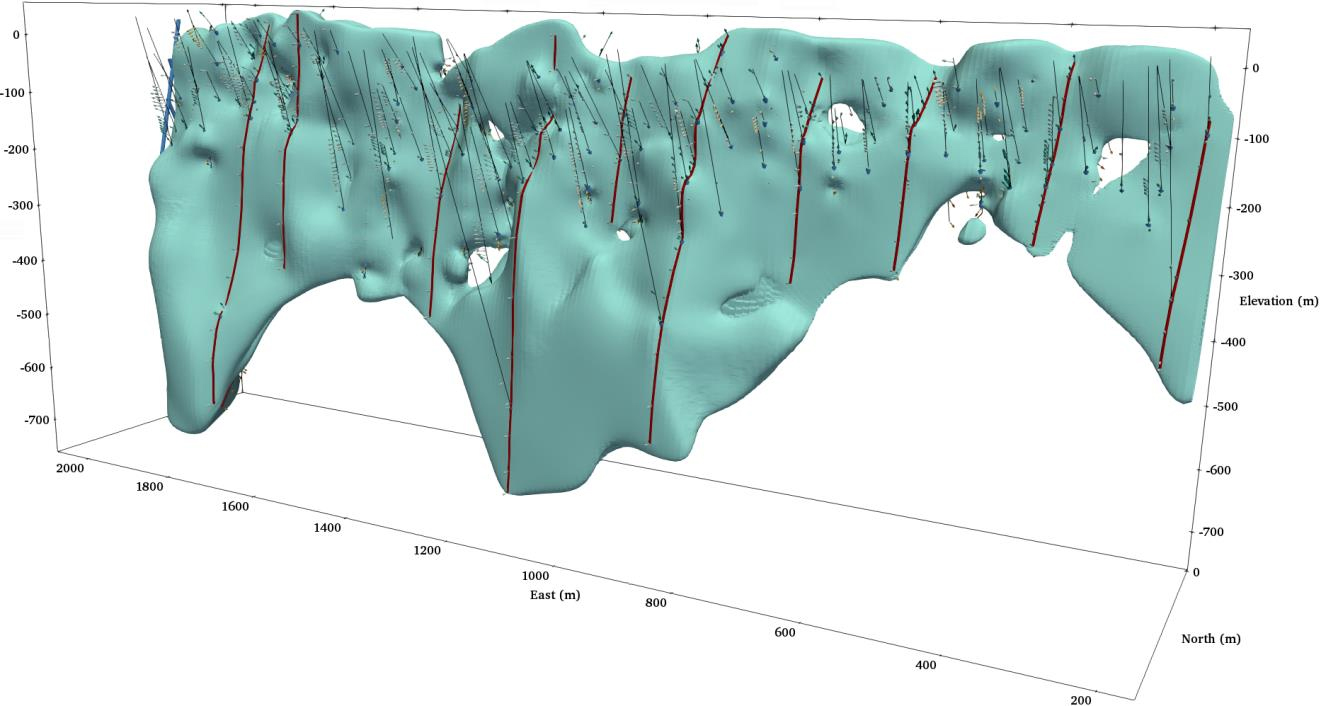
\includegraphics[width=0.8\textwidth]{capitulo_2/modelo_mls.jpg}\label{b}}
\legend{Fonte: \citeonline{manchuck_MLS}}
\end{center}
\end{figure}

A incerteza pode ser avaliada pelo método por meio do parâmetro de incerteza C e simulações não condicionais. 

Apesar da integração furos/interpretação ser muito promissora já que são duas fontes de dados que serão utilizadas na geração do modelo. O método é recente e ainda apresenta alguns desafios operacionais, principalmente em relação à exigência de estruturas planares e avaliação de incerteza.

\section{Avaliação da incerteza}

Sempre existirá algum grau de incerteza nos volumes geológicos modelados, que varia de acordo com o número de amostras e a informação geológica disponível. A incerteza do modelo geológico, muitas vezes, pode ser a maior fonte de incerteza do projeto mineiro. Por esse motivo, diversos métodos foram desenvolvidos com o objetivo de avaliar a incerteza dos modelos geológicos a partir das funções distância assinaladas.

Essa seção abordará os métodos disponíveis na literatura com exemplos práticos no banco de dados apresentado.

\subsection{Avaliação heurística da incerteza}\label{heuristic}

O método mais simples de avaliação de incerteza em modelos geológicos implícitos, proposto por \citeonline{silvaanddeutschccgmodeling}, consiste em transformar distâncias estimadas em probabilidades via \textit{softmax transformation}. Técnica amplamente usada em métodos de classificação para múltiplas classes \cite{mccullaghgeneralizedlinear}. A ideia é transformar as distâncias estimadas em probabilidades a partir da \autoref{eq_softmax}. Os valores transformados encontram-se entre zero e um e  sua soma deve ser igual a um, para cada bloco estimado.

\begin{equation}
	P(i(u)=k)=\frac{e^\frac{-d^*_k(u)}{\gamma}}{\sum_{k'=1}^{K}e^\frac{-d^*_k(u)}{\gamma}}
    \label{eq_softmax}
\end{equation}

$P(i(u)=k)$ representa a probabilidade de um local $u$ pertencer à categoria $k$, $d^*_k(u)$ é a distância estimada para a categoria $k$ e $\gamma$ é um parâmetro que regula a inter-relação entre as probabilidades das $K$ diferentes categorias. Quanto maior $\gamma$, maior as diferenças entre as probabilidades (maior a banda de incerteza), como pode ser observado na \autoref{softmax_ex}. \citeonline{silvaanddeutschccgcorrecting} advogam que o parâmetro pode ser a maior distância estimada entre todas as categorias.

Para exemplificar a transformação, a \autoref{softmax_grafico}, mostra à esquerda as distâncias estimadas para cada uma de cinco categorias em um mesmo bloco em particular. À direita as distâncias transformadas pela \autoref{eq_softmax} em probabilidades daquele bloco pertencer a cada uma das cinco categorias. Observe que distâncias menores (mais negativas) geram probabilidades maiores, e vice-versa.  

\begin{figure}[!ht]
	\caption{\label{softmax_grafico}Distâncias estimadas e transformadas em probabilidades para um mesmo bloco.}
	\begin{center}
		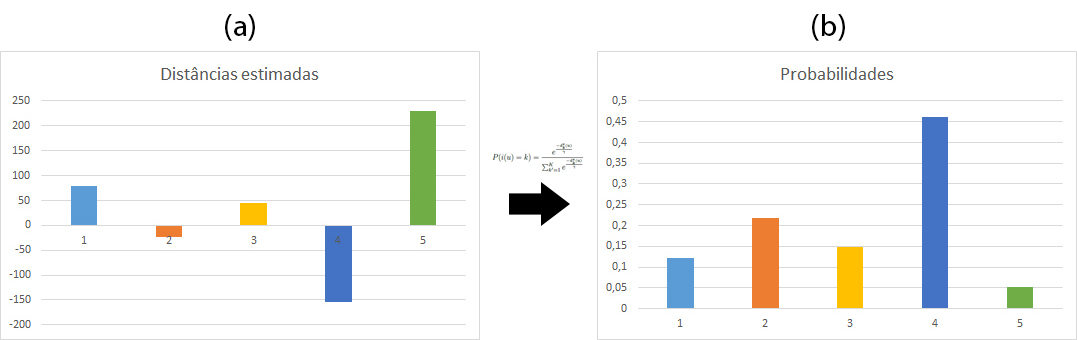
\includegraphics[width=0.7\textwidth]{capitulo_2/softmax_bars_final.jpg}
	\end{center}
	\legend{Fonte: \citeonline{rolo_dissertacao}}
\end{figure}

A \autoref{softmax_ex} mostra seções em XZ do mapa de probabilidades para a categoria 1, com diferentes valores para $\gamma$.

\begin{figure}[t]
\caption{Seções em XZ do mapa de probabilidades para a categoria 1 com diferentes valores para $\gamma$.} 
\label{softmax_ex}
\begin{center}
\subfloat[][$\gamma=30$]{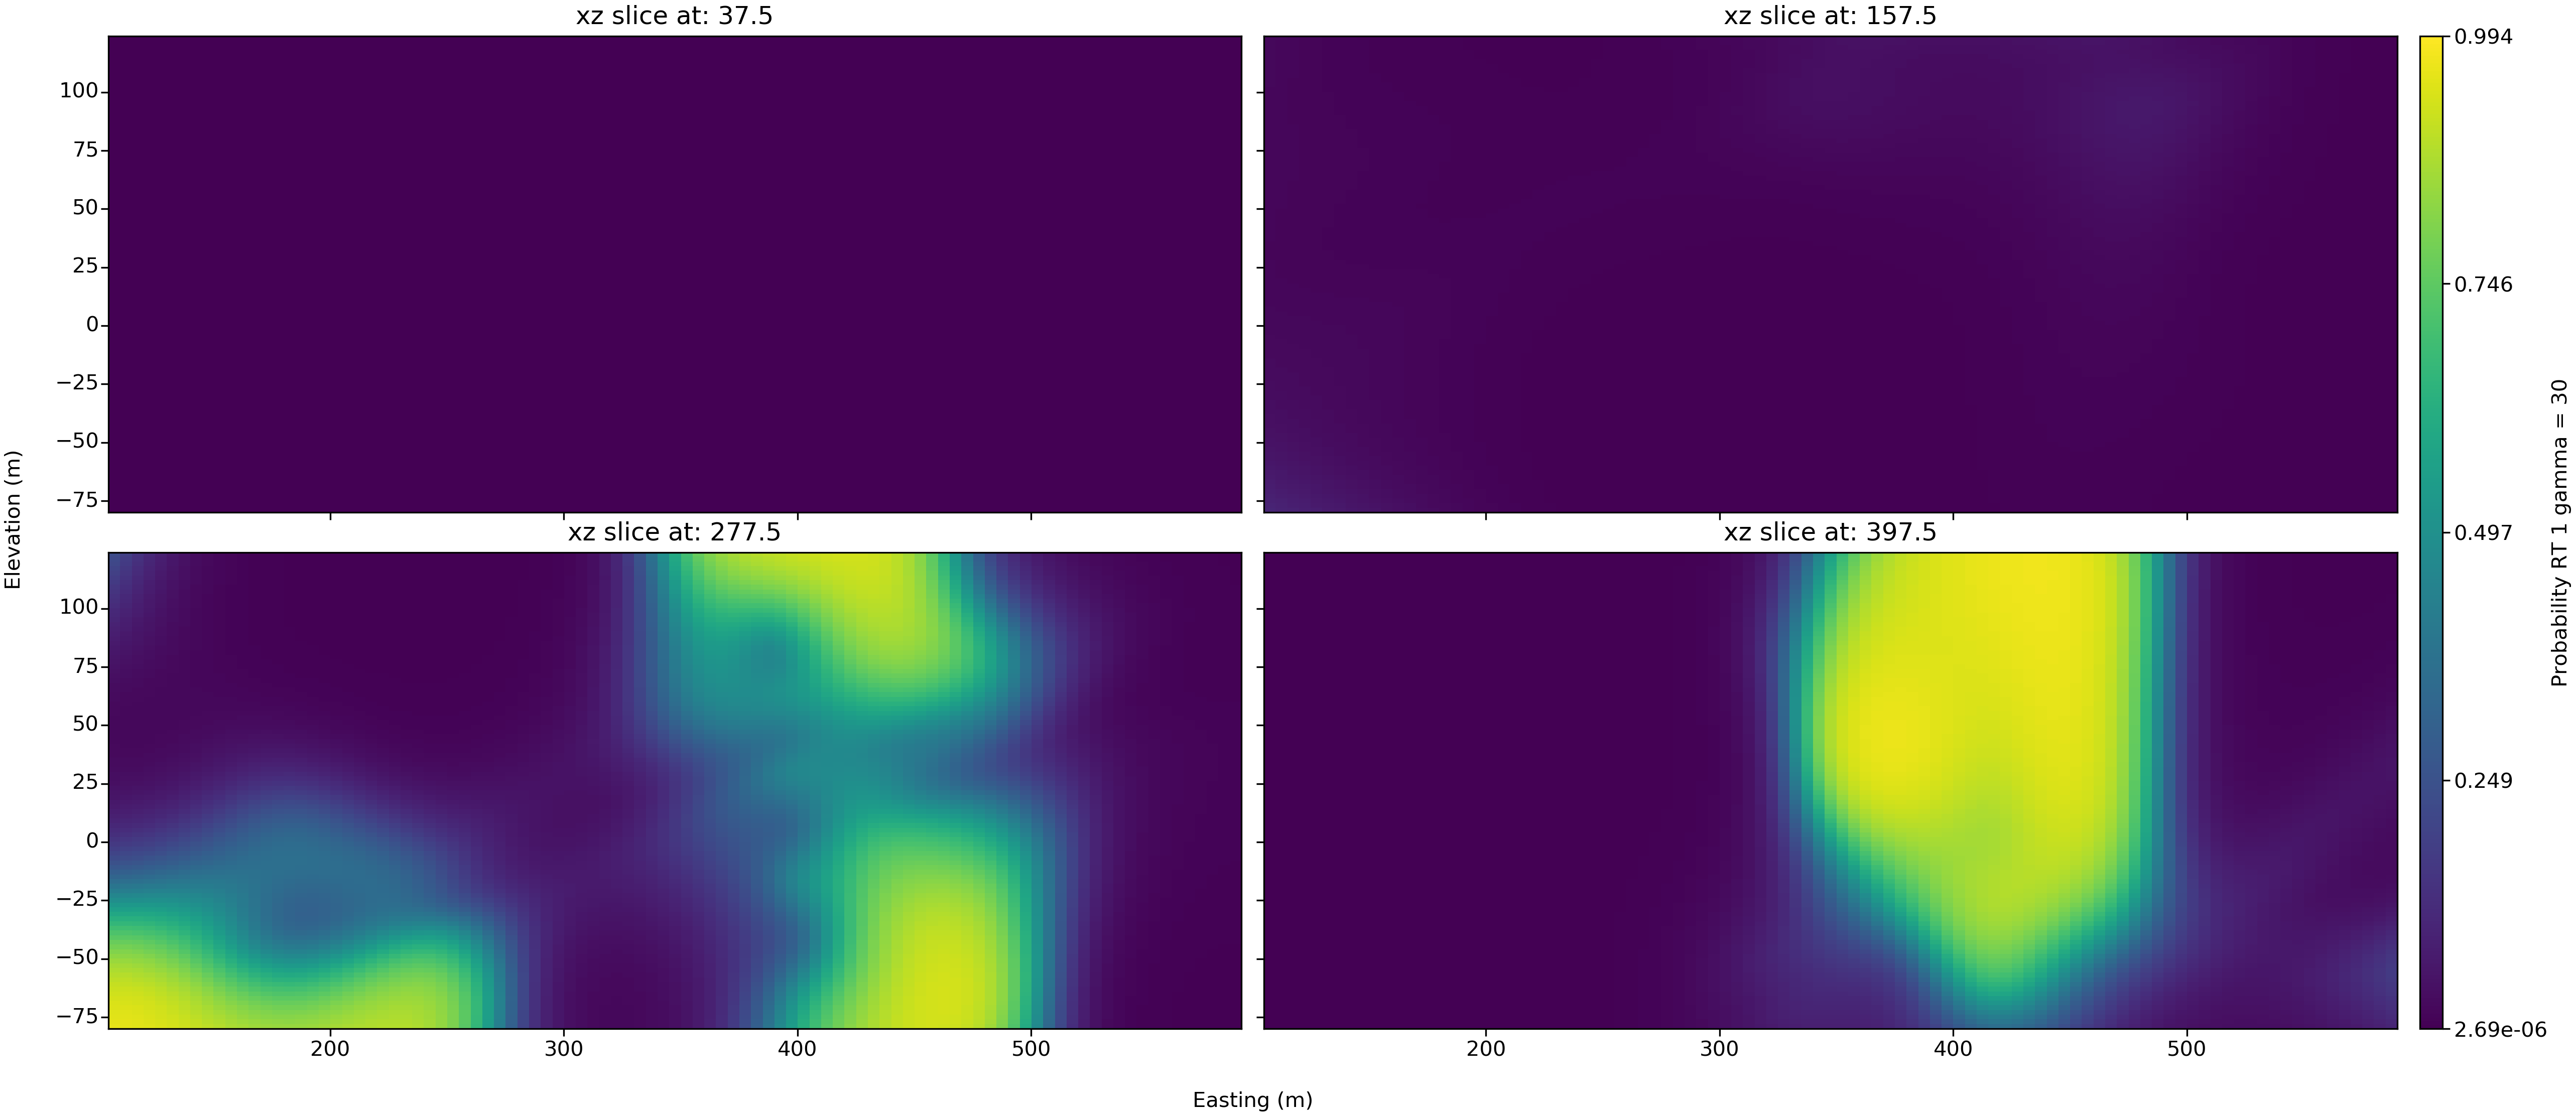
\includegraphics[width=0.8\textwidth]{capitulo_2/xz_30.png}\label{a}}\\
\end{center}
\begin{center}
\subfloat[][$\gamma=50$]{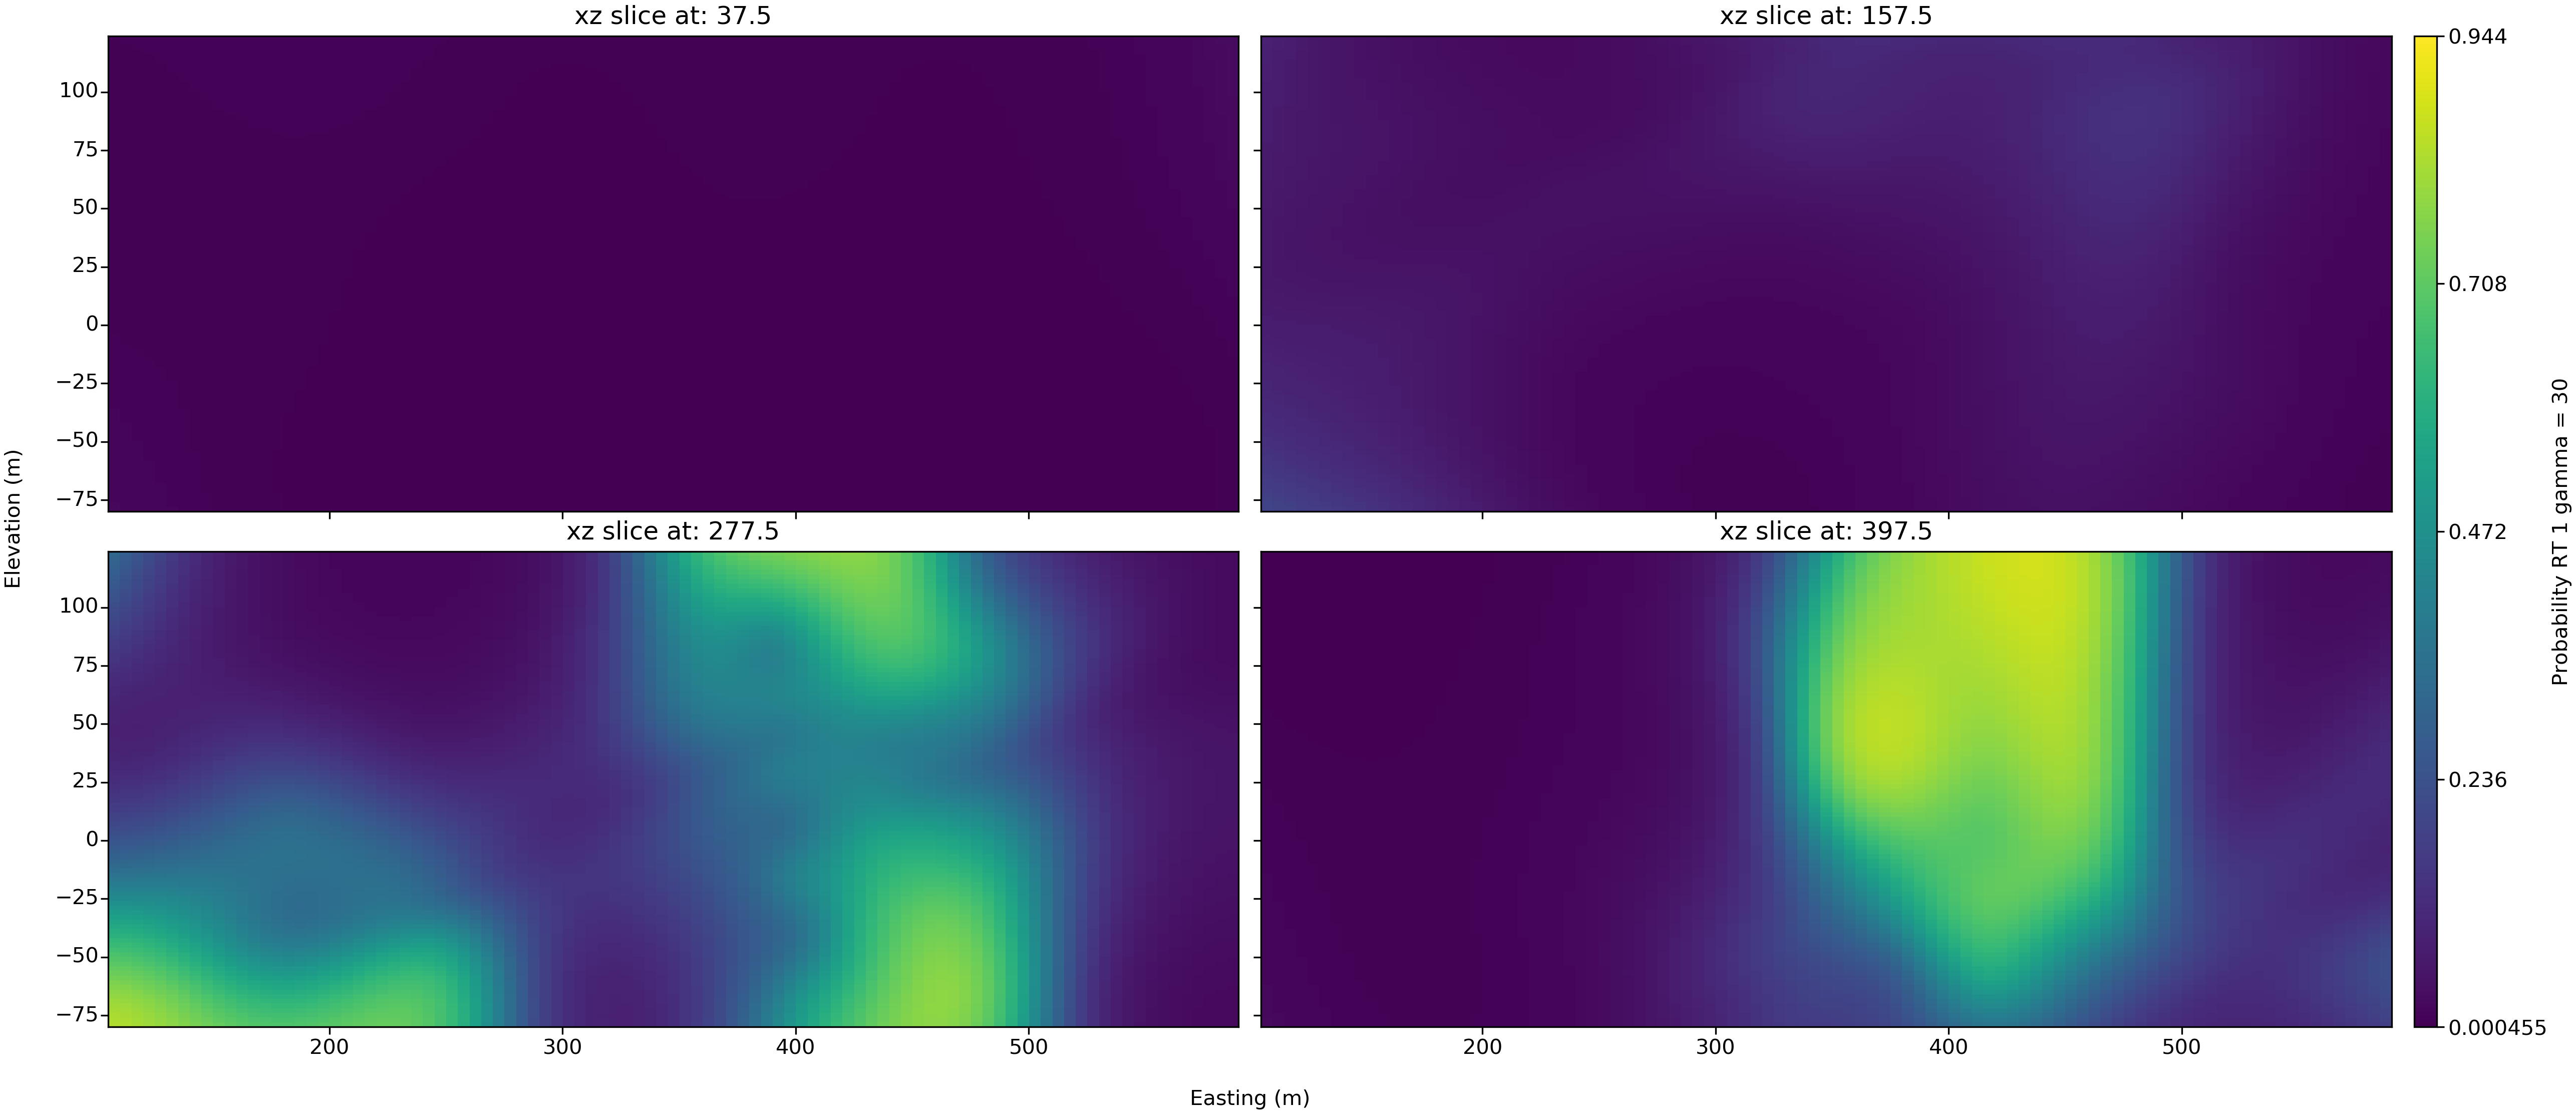
\includegraphics[width=0.8\textwidth]{capitulo_2/xz_50.png}\label{b}}
\end{center}
\end{figure}

Apesar do método ser simples e direto, suportar múltiplas categorias simultaneamente, seu resultado não pode ser utilizado em etapas subsequentes do processo de  avaliação, por não gerar múltiplas realizações do modelo geológico. Além disso, A escolha do parâmetro $\gamma$ é subjetiva e dependa da distribuição espacial das amostras, dependendo da escolha para o parâmetro nem mesmo blocos colocados com amostras recebem a probabilidade 100\%. 

\subsection{\textit{Boundsim}}

Uma outra metodologia proposta por \citeonline{mclennan2006boundsim} consiste em realizar um \textit{bootstrap} espacial \cite{deutsh_spatial_bootstrap} da média da distância assinada calculada para uma dada categoria. O procedimento de \textit{bootstrap} é amplamente utilizado para quantificar incerteza em parâmetros estatísticos, As duas mais importantes suposições são: os dados são representativos e os dados são independentes. Por esse motivo, a técnica de amostragem deve ser modificada para variáveis que apresentam continuidade espacial. A \autoref{bs_df_1} mostra o histograma da média para as distâncias assinaladas da categoria 1 do banco de dados. 

\begin{figure}[!ht]
	\caption{\label{bs_df_1}Histograma do bootstrap espacial da média das distâncias assinaladas para a categoria 1.}
	\begin{center}
		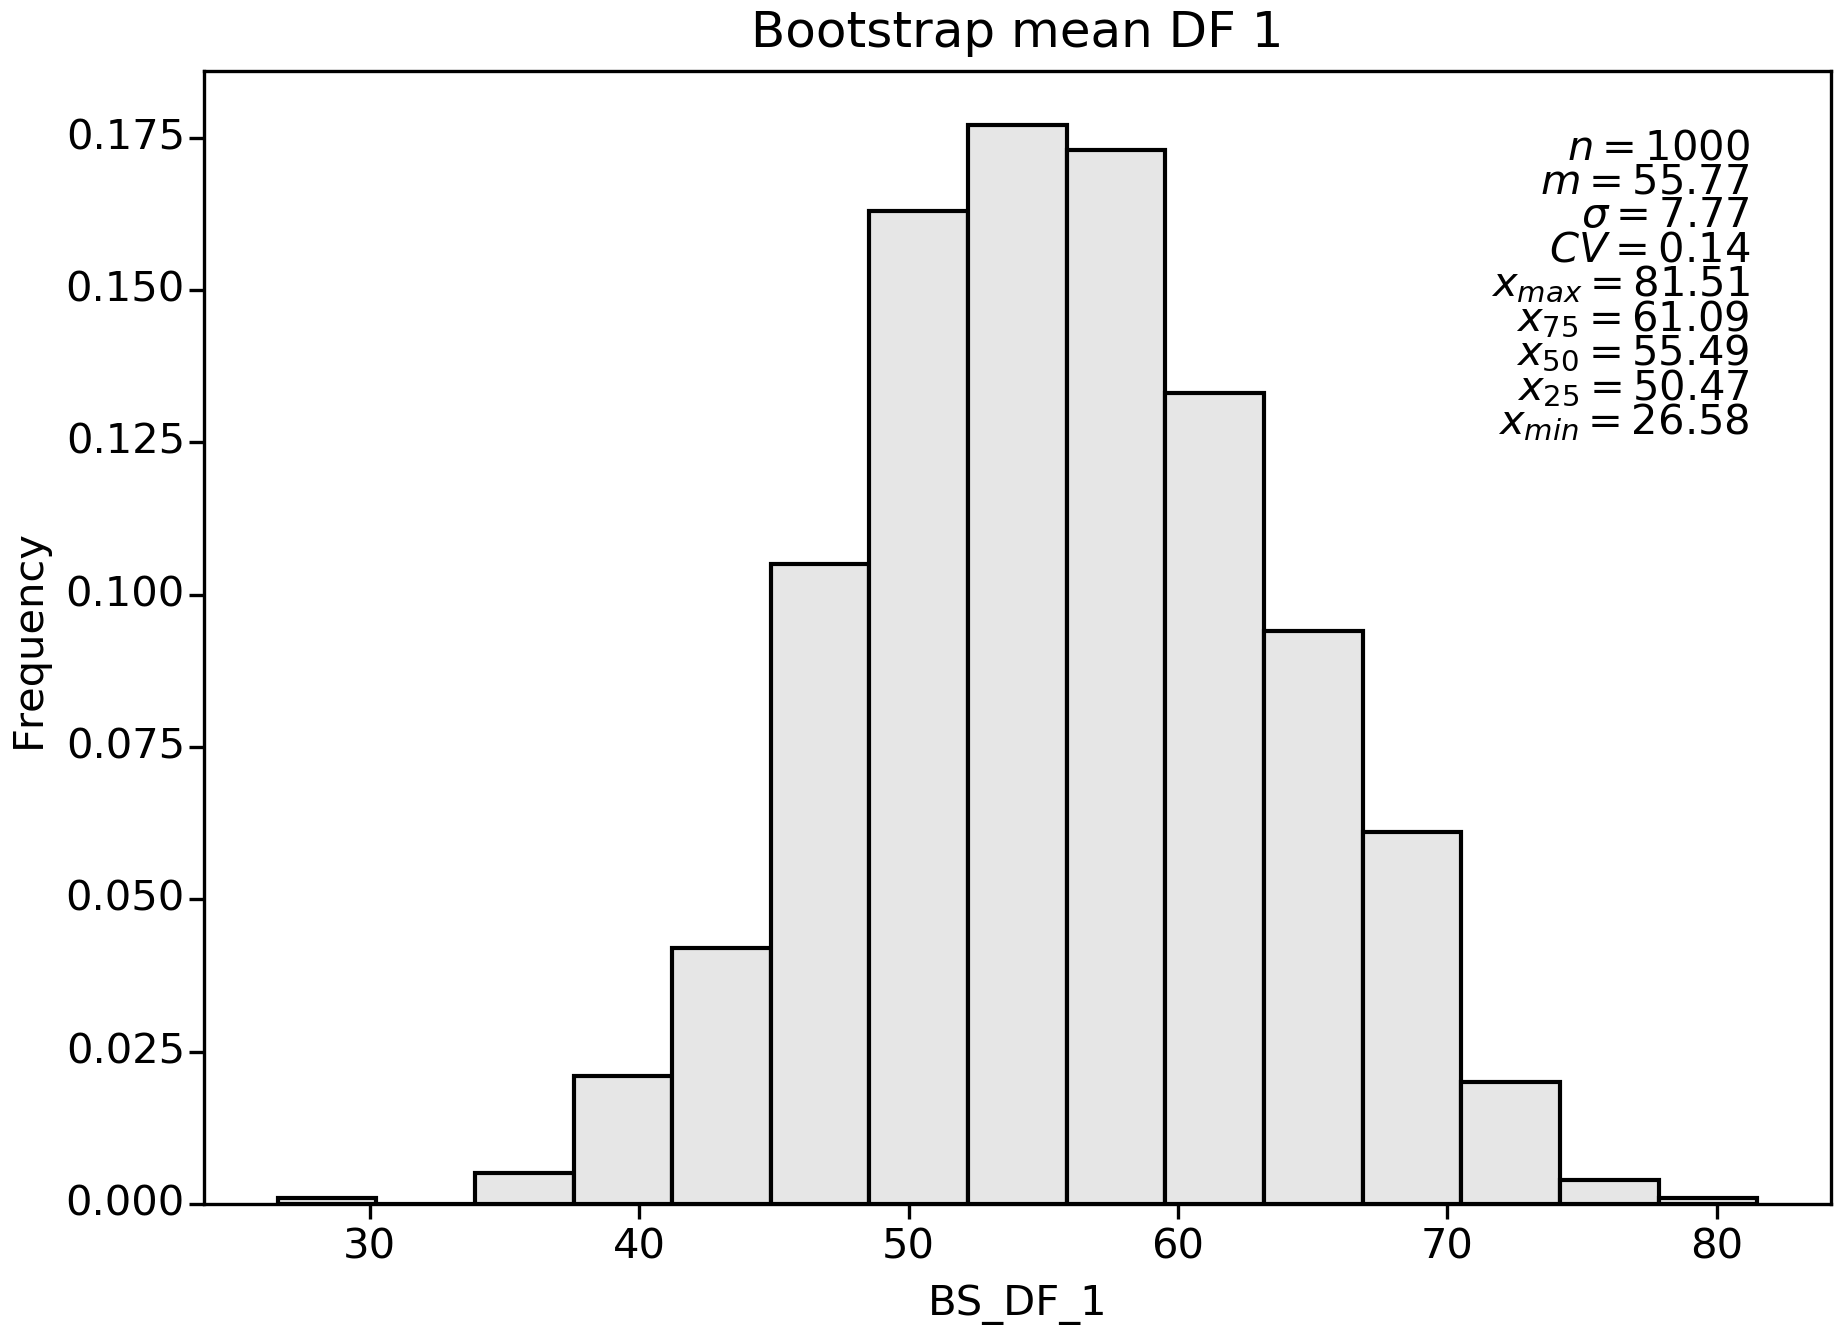
\includegraphics[width=0.5\textwidth]{capitulo_2/BS_DF_1.png}
	\end{center}
	%\legend{Fonte: \citeonline{rolo_dissertacao}}
\end{figure}

Valores para a média são tomados do histograma da média, gerado pelo \textit{bootstrap} espacial. Esses valores podem ser correspondentes ao p10, p50 e p90 por exemplo.

Então, as distâncias assinaladas são interpolados para os nós do grid por krigagem simples, que tem como hipótese a estacionariedade da média por todo o domínio. A média estacionária para a krigagem simples são os valores tomados do histograma.

O último passo consiste em extrair a iso superfície zero dos modelos implícitos gerados por krigagem simples com os diferentes valores da média estacionária tomadas do histograma da média. Em tese, quanto maior o percentil menor o risco associado, o volume do sólido modelado infla ou contrai de acordo com o valor escolhido para a média estacionária.

A \autoref{boundsim_table} mostra os blocos classificados como pertencentes à categoria 1 usando a metodologia apresentada, com valores de média estacionária correspondentes à p10, p50 e p90.

\begin{table}[]
\begin{center}
\begin{tabular}{lr}
Percentil & \multicolumn{1}{l}{Blocos dentro} \\ \hline
10 & 109886 \\
50 & 110446 \\
90 & 111069 \\ \hline
\end{tabular}
\end{center}
\caption{Blocos classificados como pertencentes à categoria 1.}\label{boundsim_table}
\end{table}

A metodologia é simples e direta, porém, deve ser aplicada à uma categoria por vez, na presença de múltiplos domínios alguma abordagem hierárquica deve ser estabelecida. A sensibilidade da krigagem simples à média depende da configuração espacial das amostras, muitas vezes a diferença entre os volumes obtidos é irrelevante, como no caso do banco de dados em estudo: a diferença no volume do sólido do caso mais conservador para o de maior risco é de pouco mais de 1\%. As iso superfícies são praticamente coincidentes.

O produto final do método pode ser utilizado nas etapas subsequentes do processo de avaliação, todavia, o método não avalia incerteza de forma adequada. Os autores do estudo original aplicaram a metodologia apenas em bancos de dados sintéticos e de geometria regular. 

\subsection{Simulação direta das distâncias assinaladas}\label{sim_direta}

\citeonline{caceres2011stochastic} e \cite{radtke_dissertacao} propuseram que as distâncias assinaladas sejam simuladas de forma direta: a partir de um modelo geológico implícito multi categórico (\autoref{multi_cat}) um coeficiente U de incerteza deve ser calculado de acordo com \autoref{u_eq}:

\begin{equation}\label{u_eq}
    U(u)=\frac{max\{D_{min}\}-min\{d^*_k(u)\}^K_{k=1}}{max\{D_{min}\}-min\{D_{min}\}}
\end{equation}

Onde:

\begin{equation}
    D_{min}=\{min\{d^*_k(u_1)\},...,\{min\{d^*_k(u_n)\}^K_{k=1}\}
\end{equation}

E $d^*_k(u)$ é a distância estimada no local u para a categoria k.

Os valores de U variam entre 0 e 1, um \textit{cutoff} em U determina a extensão da zona de incerteza ao redor dos contatos: quanto mais próximo de 1, mais estreita a zona. A \autoref{u_fig} mostra o coeficiente U calculado para todos os nós do grid a partir do modelo da \autoref{multi_cat_rbf}.

\begin{figure}[!ht]
	\caption{\label{u_fig}Coeficiente U calculado para todos os nós do grid.}
	\begin{center}
		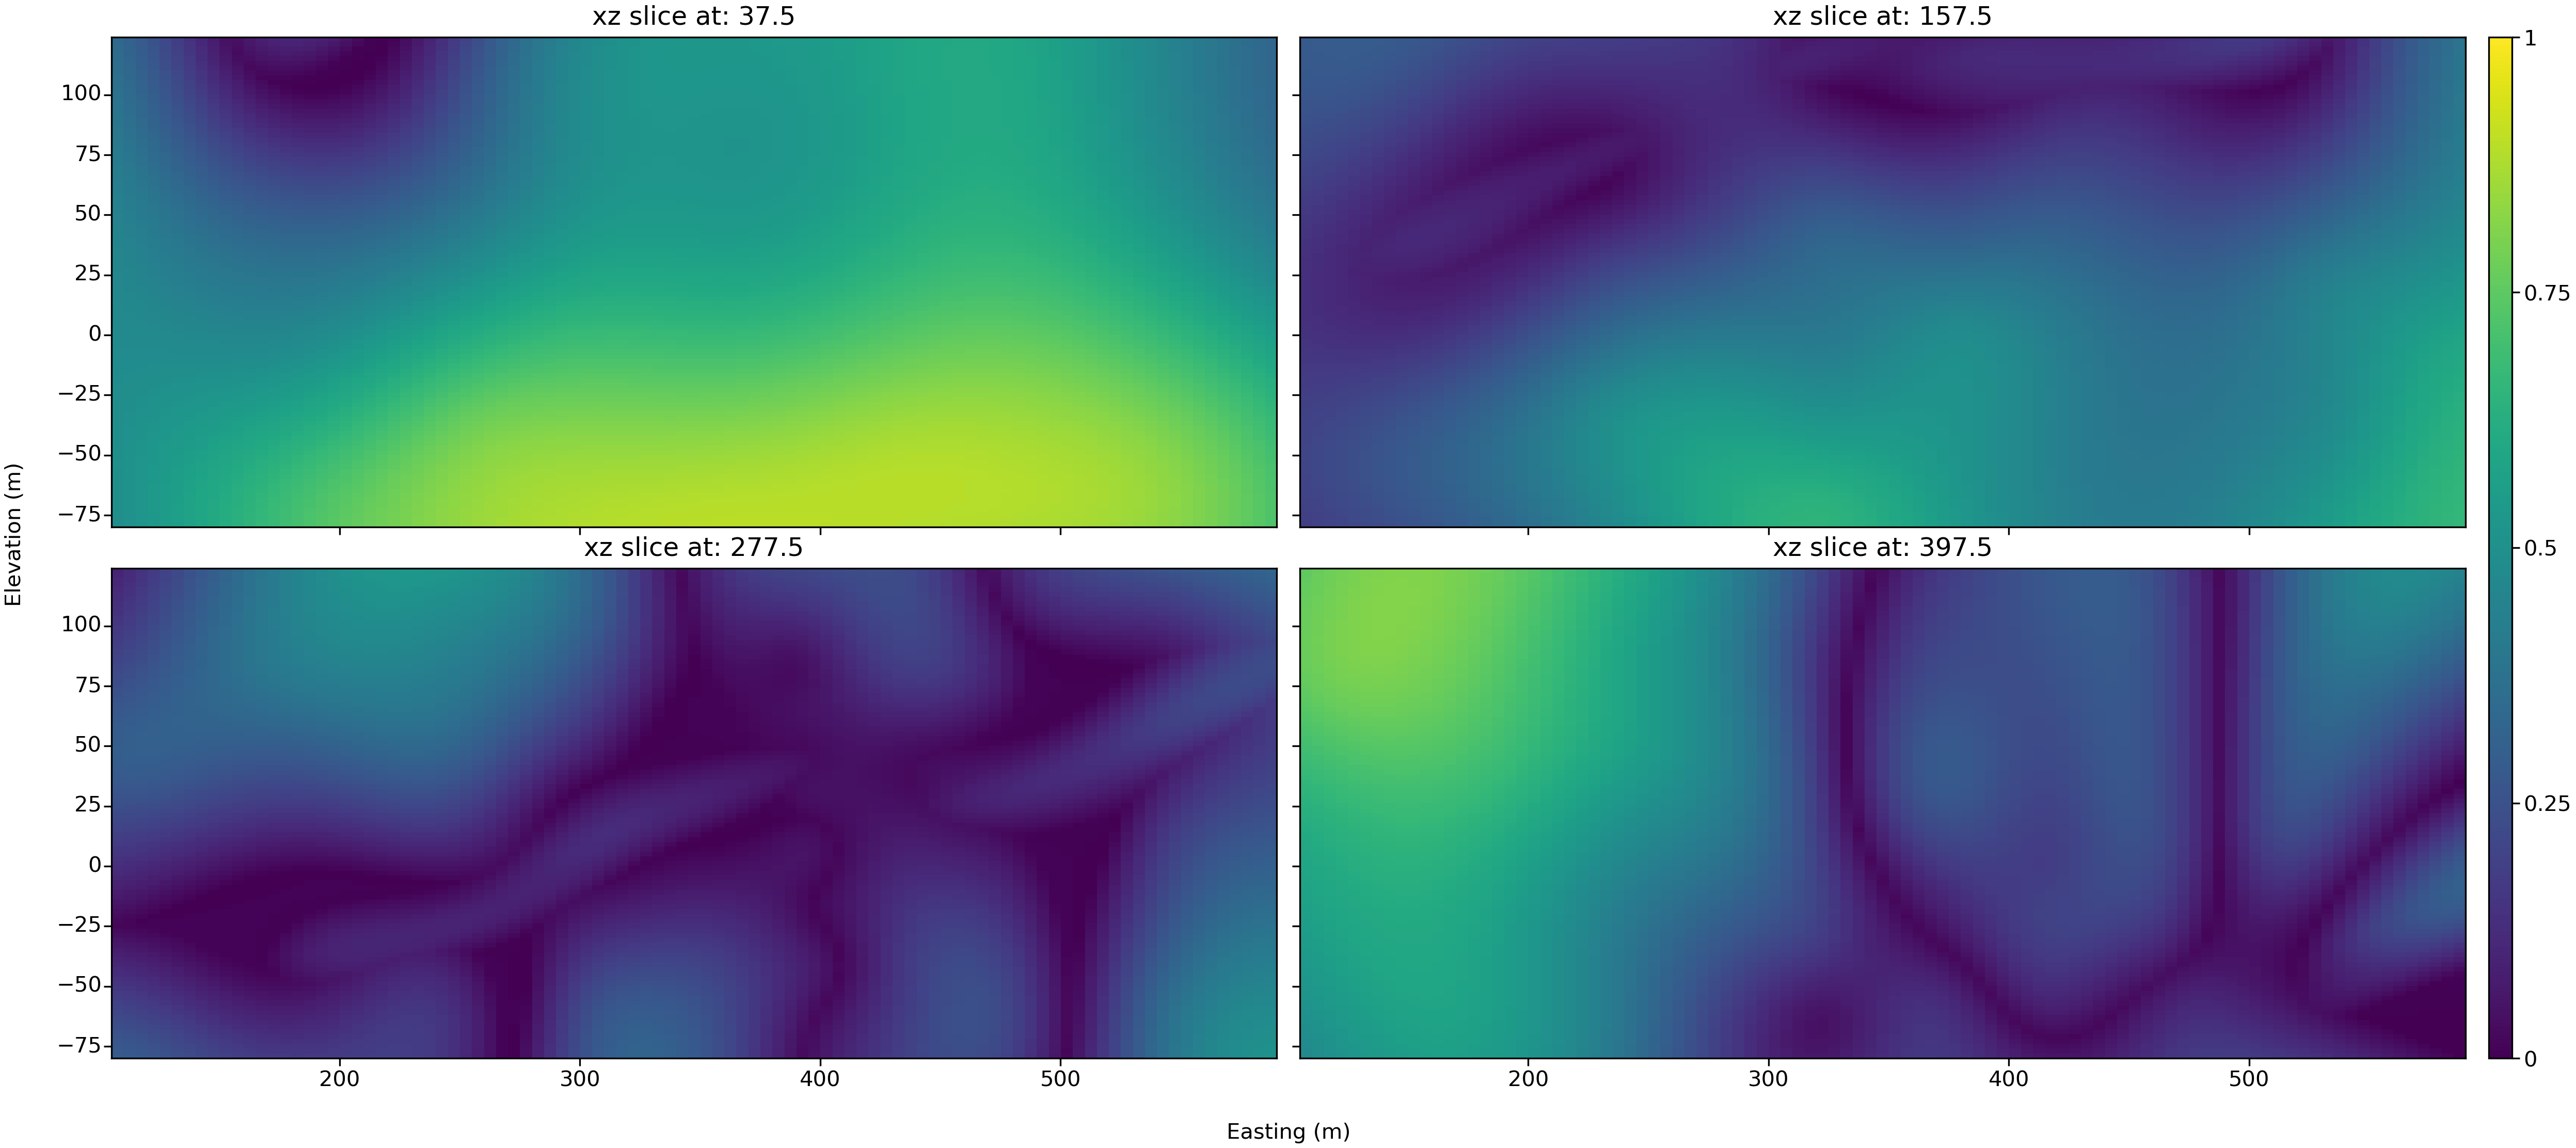
\includegraphics[width=0.8\textwidth]{capitulo_2/u_coef.png}
	\end{center}
	%\legend{Fonte: \citeonline{rolo_dissertacao}}
\end{figure}

Um \textit{cutoff} em 0.8 foi aplicado em U e as distâncias assinaladas foram simuladas por simulação sequencial Gaussiana na região de incerteza. A \autoref{dist_sim_u} mostra as distâncias simuladas para as três categorias do banco de dados na zona de incerteza. 

\begin{figure} 
    \caption{Distâncias simuladas na zona de incerteza para as categorias do banco de dados.} \label{dist_sim_u}
     \centering
     \subfloat[][Categoria 1]{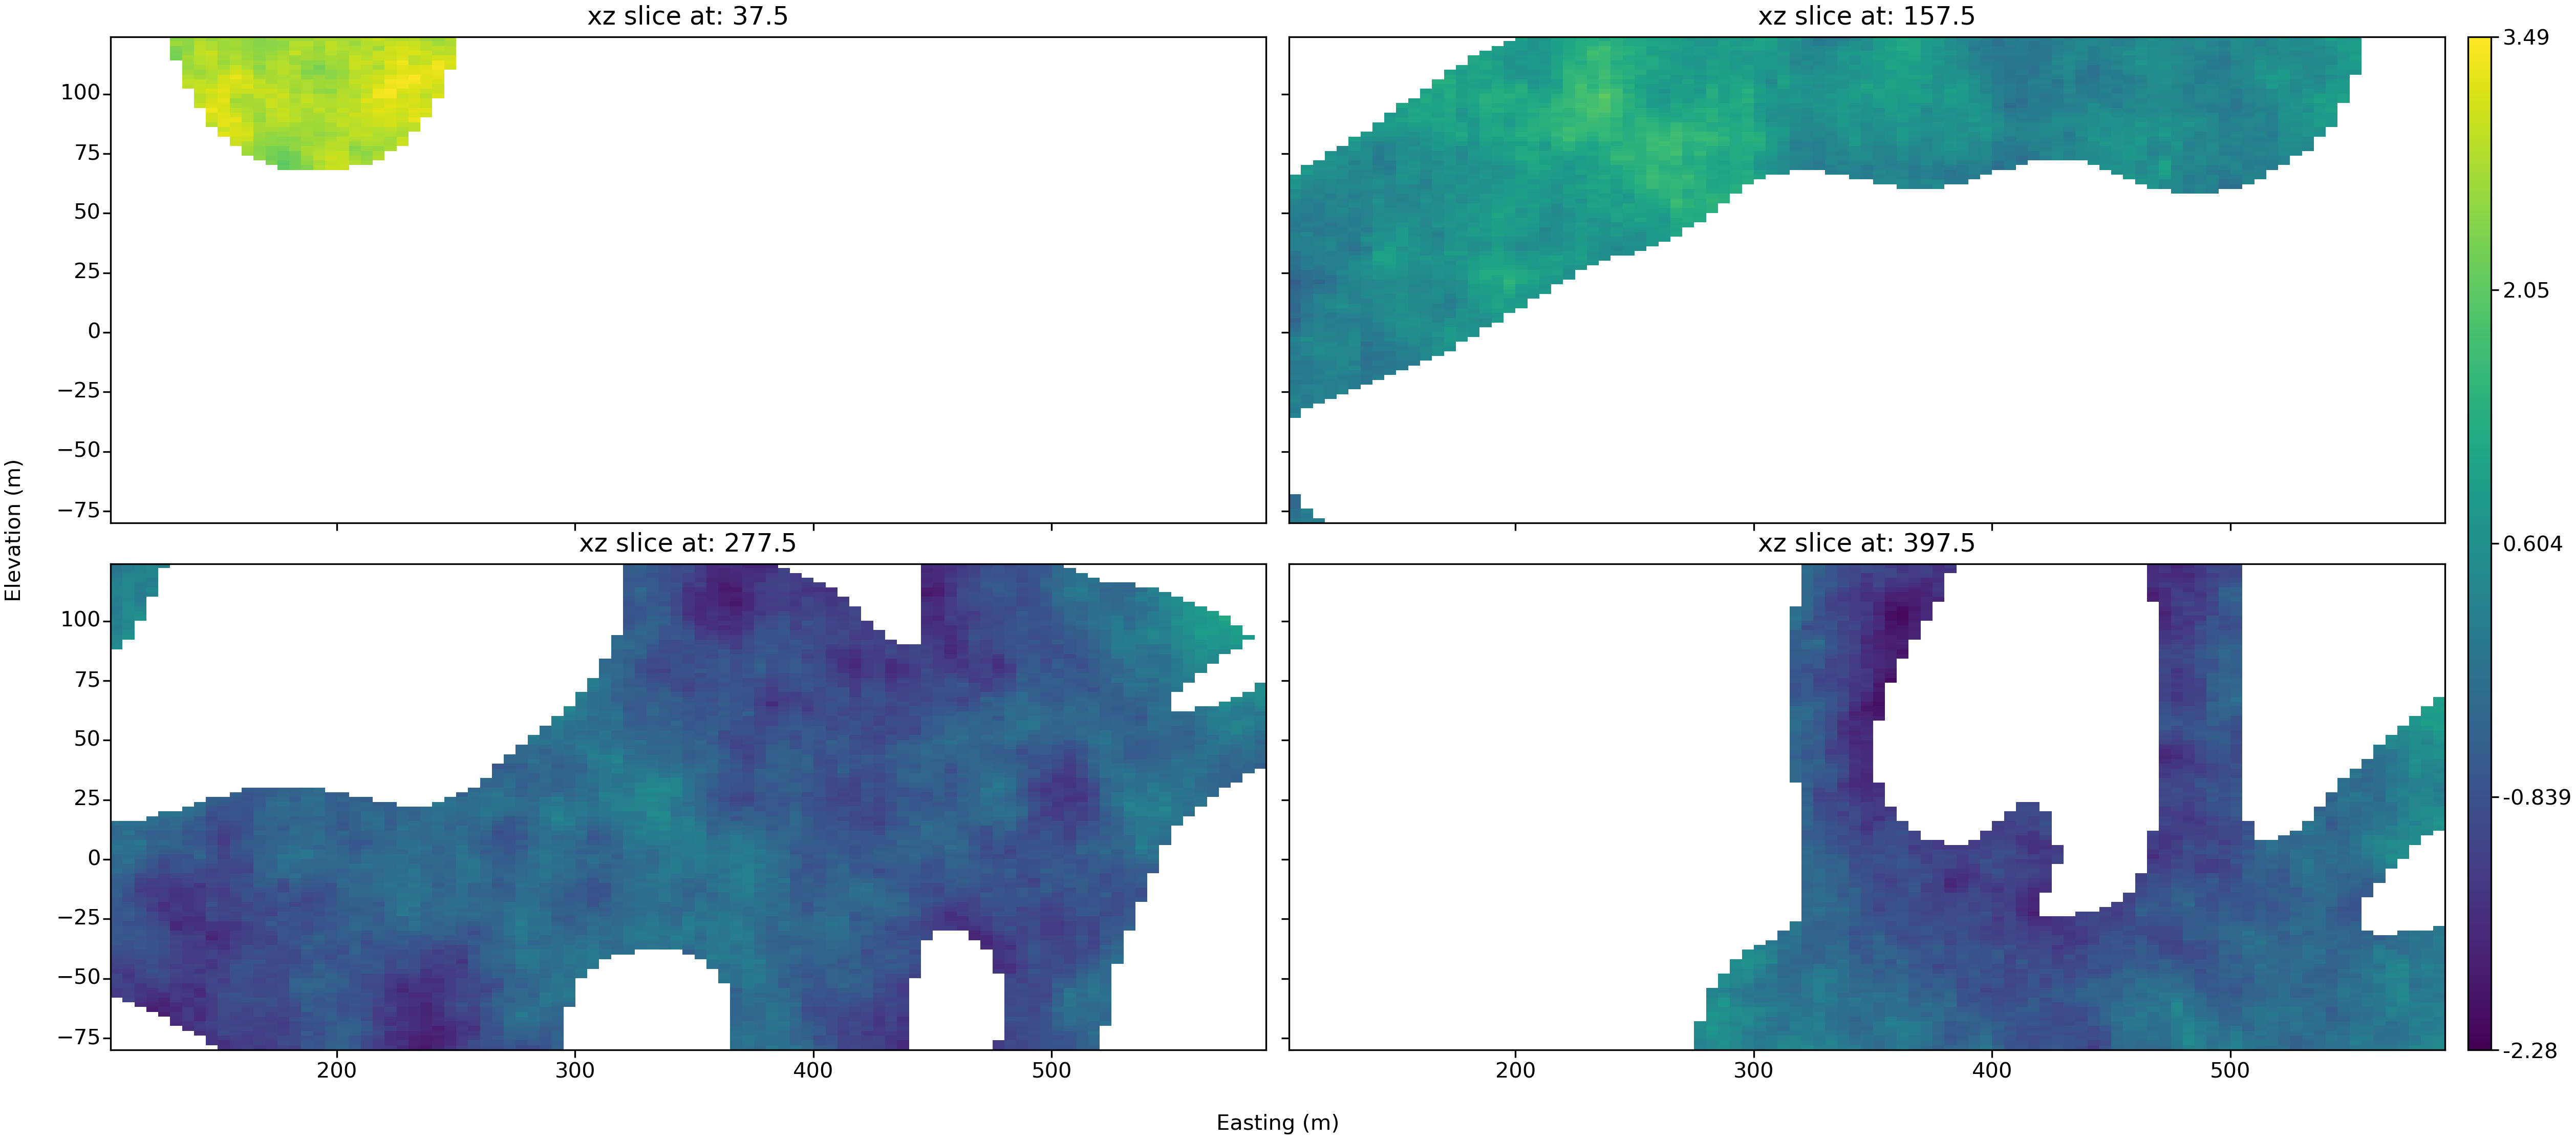
\includegraphics[width=.3\textwidth]{capitulo_2/Ucutoff1.png}\label{<figure1>}}
     \subfloat[][Categoria 2]{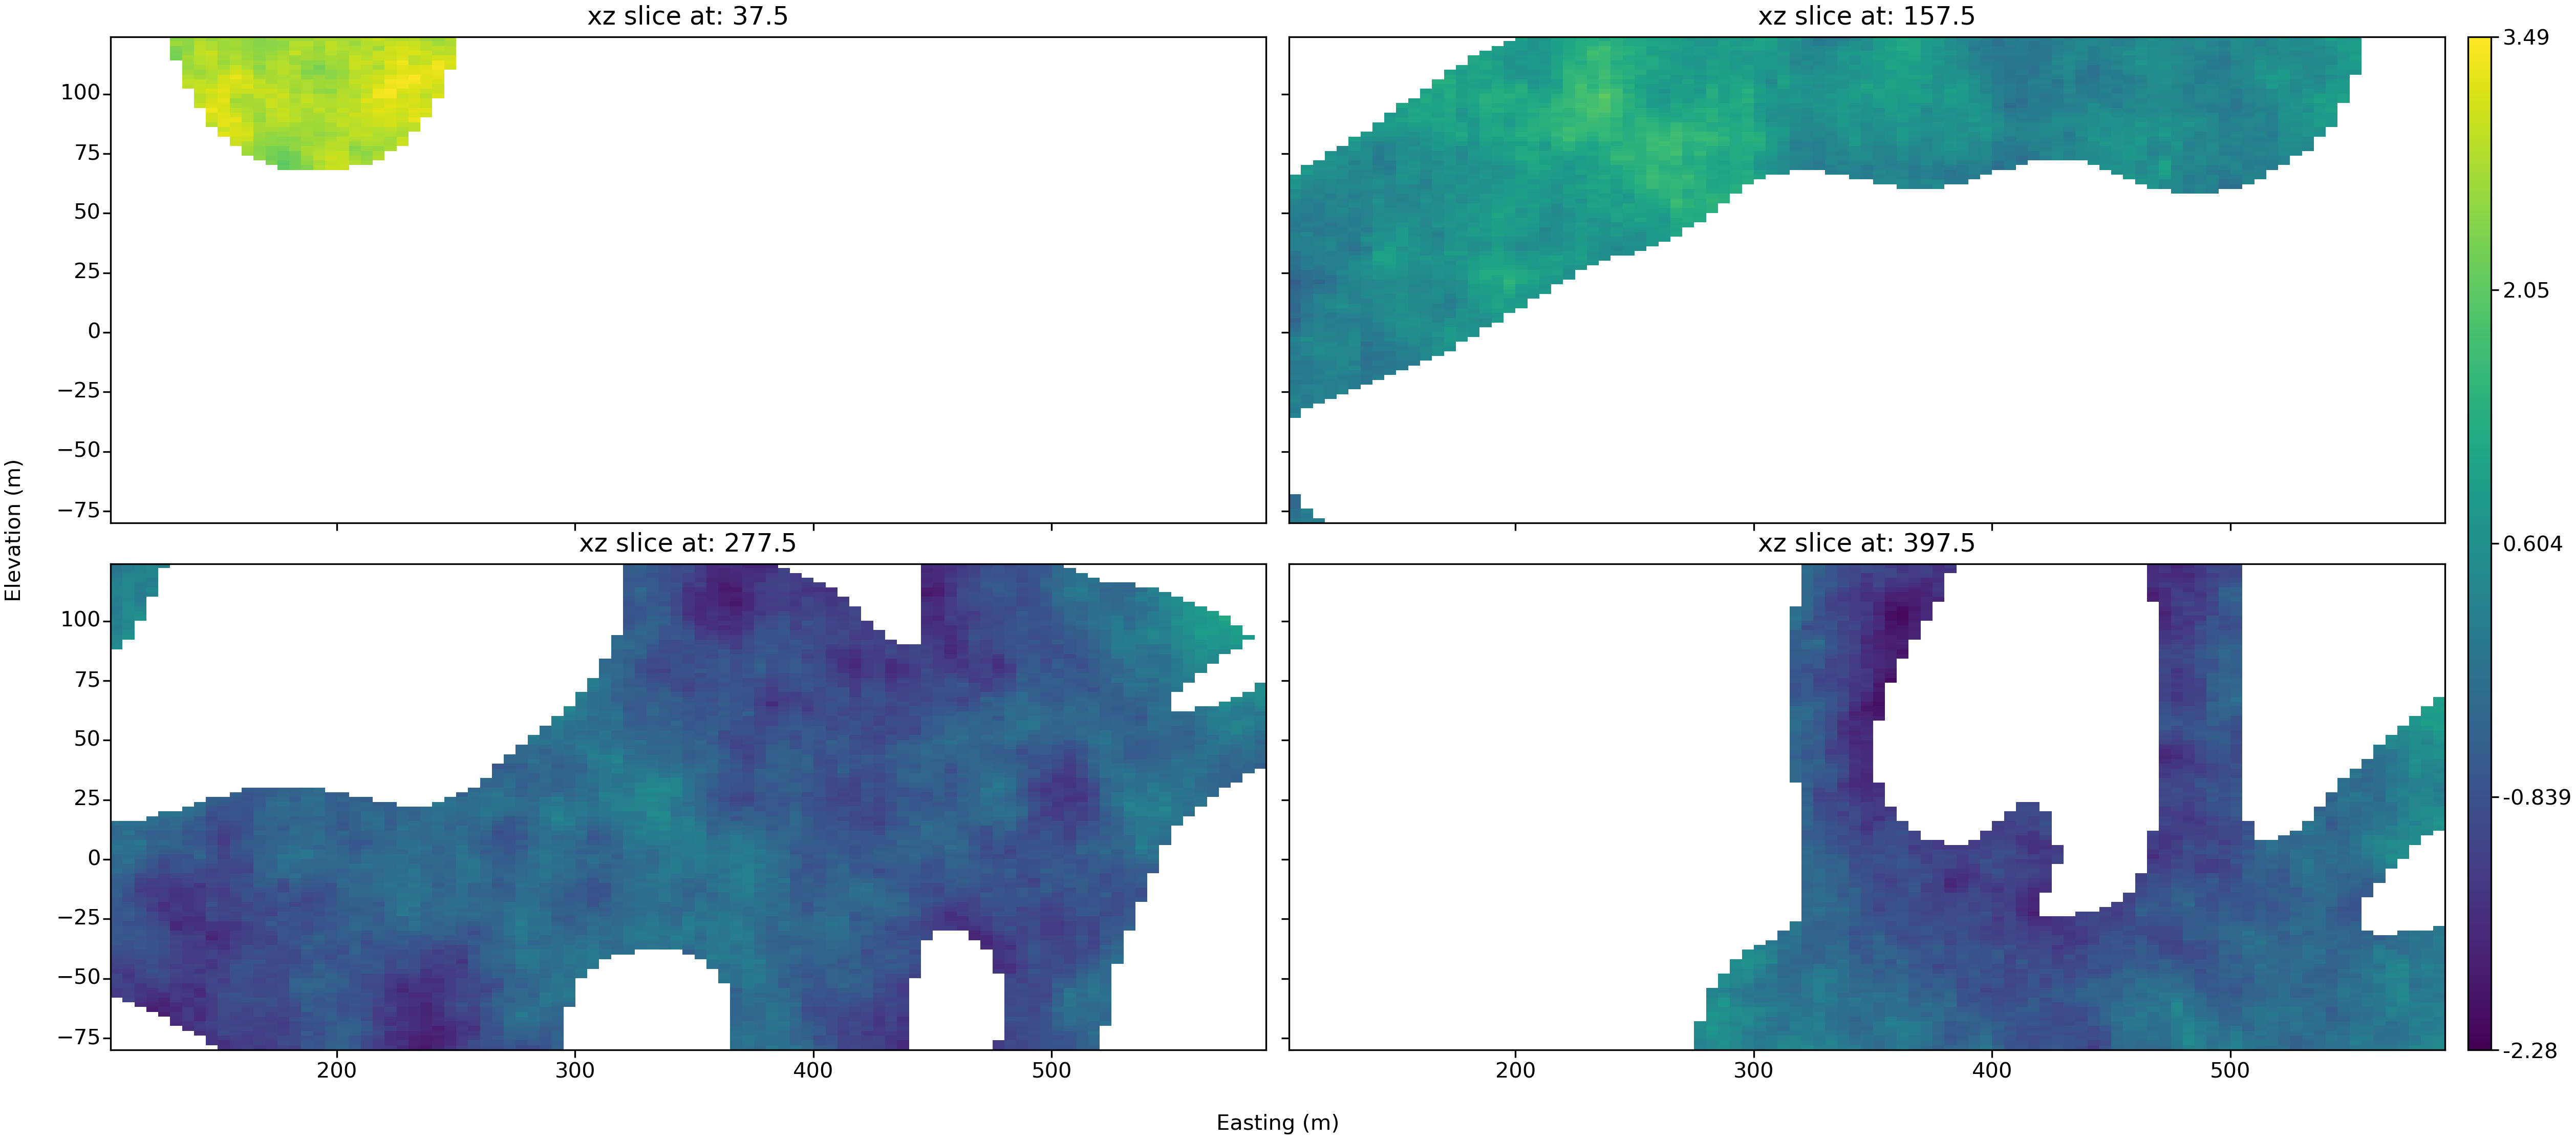
\includegraphics[width=.3\textwidth]{capitulo_2/Ucutoff2.png}\label{<figure2>}}
     \subfloat[][Categoria 3]{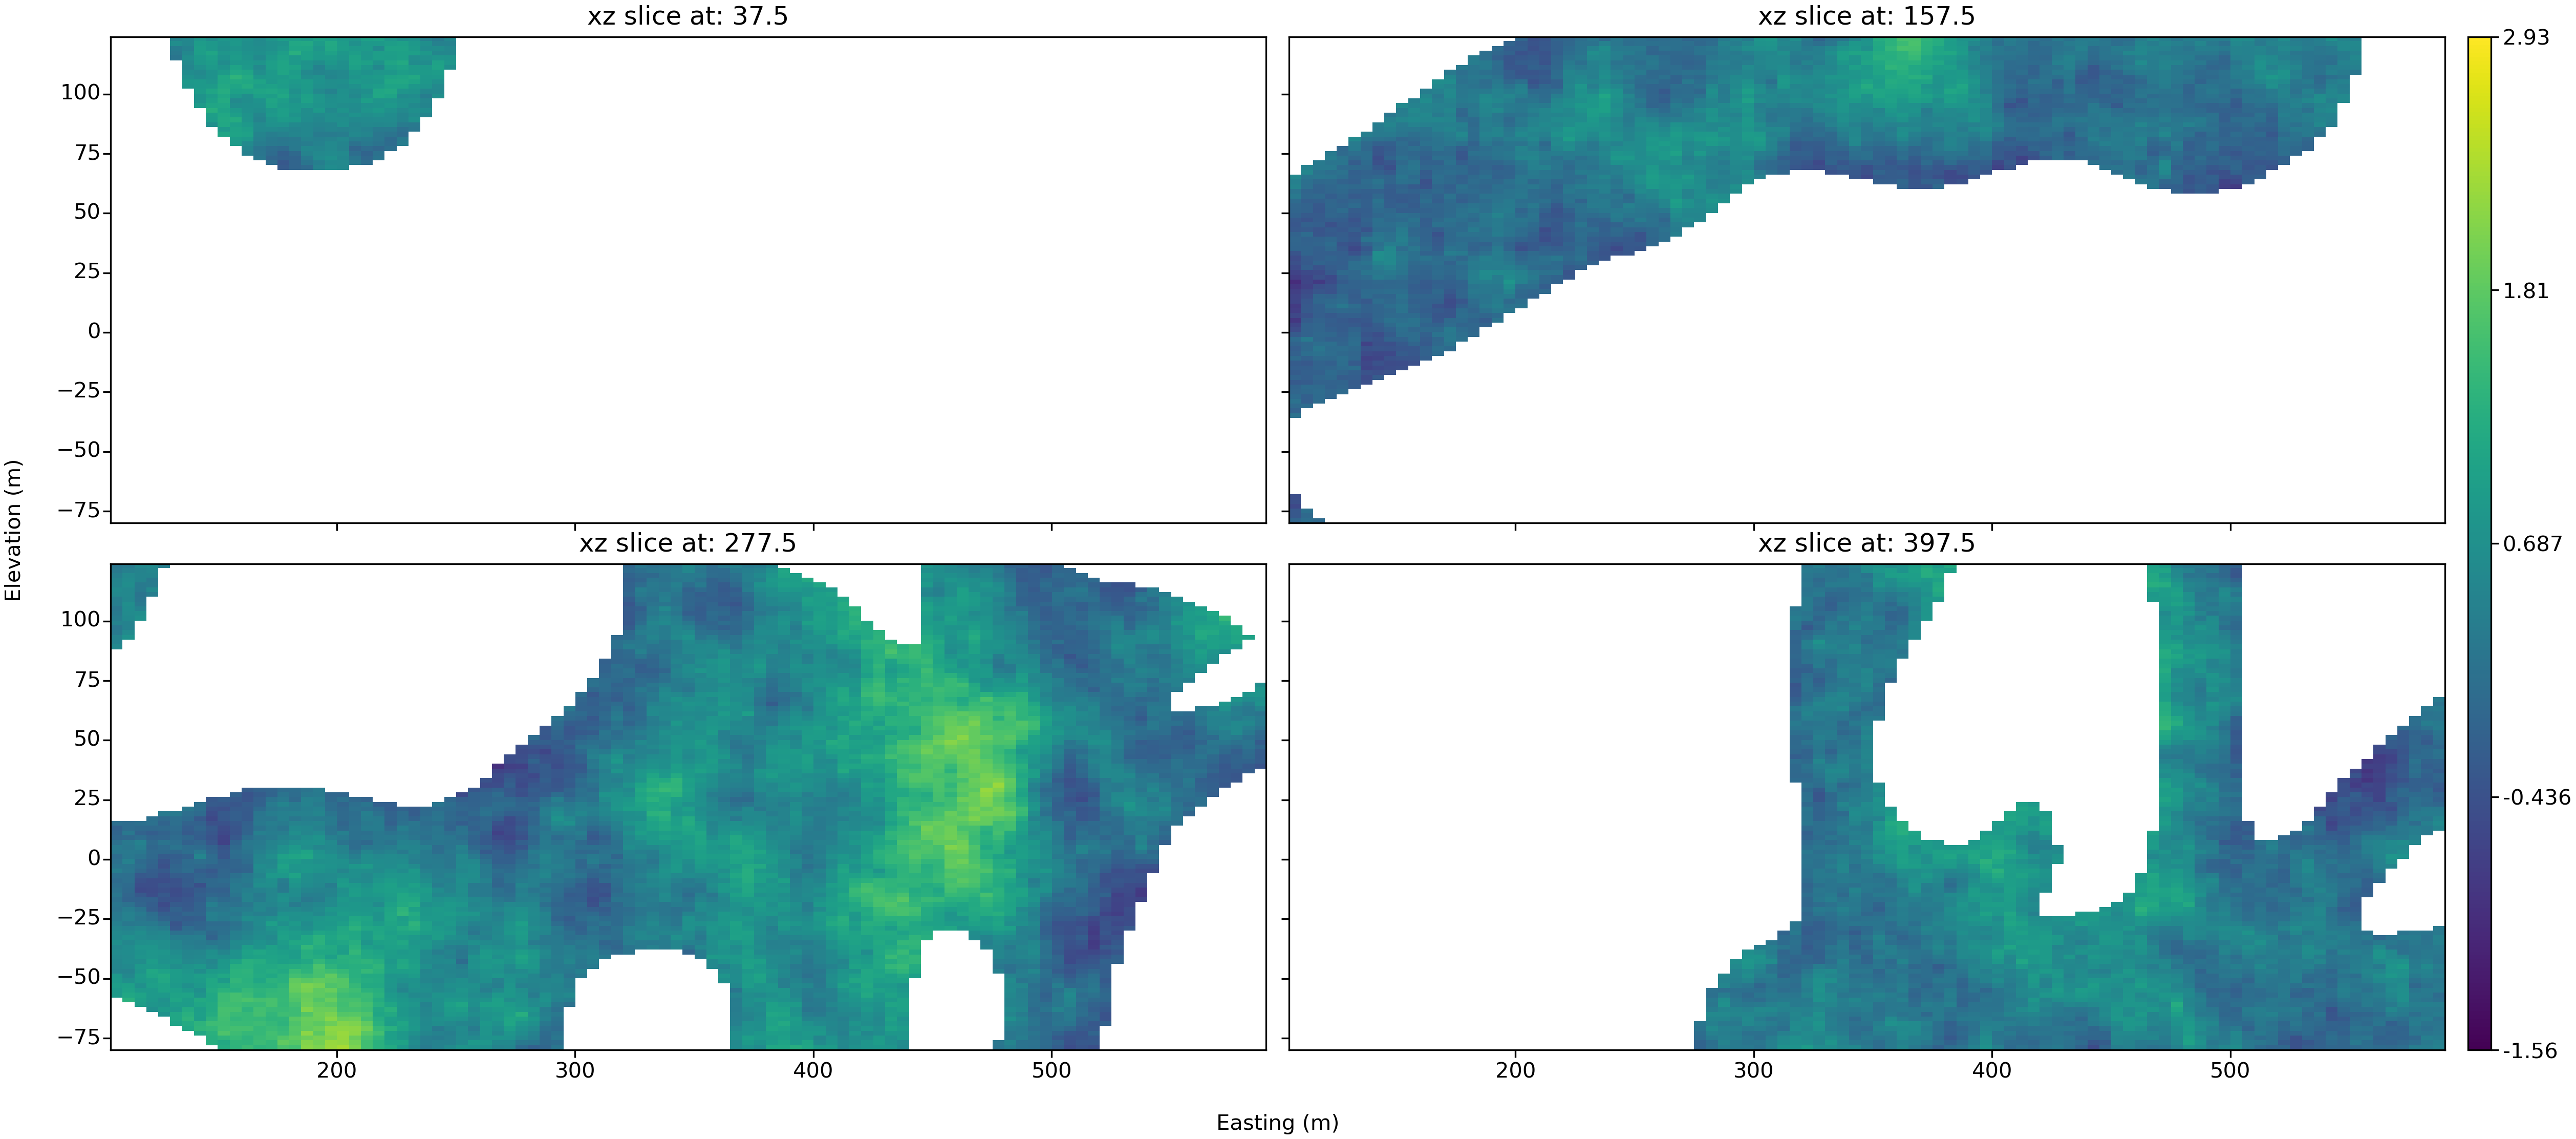
\includegraphics[width=.3\textwidth]{capitulo_2/ucutoff3.png}\label{<figure2>}}
\end{figure}

A categoria correspondente ao menor valor simulado é retida em cada bloco e os blocos simulados são concatenados com os blocos estáticos, atribuídos pela interpolação.

A \autoref{dif_real} mostra duas diferentes realizações do modelo geológico estocástico criado a partir da simulação direta das distâncias.

\begin{figure}[t]
\caption{Diferentes realizações do modelo geológico.} 
\label{dif_real}
\begin{center}
\subfloat[][Realização 1]{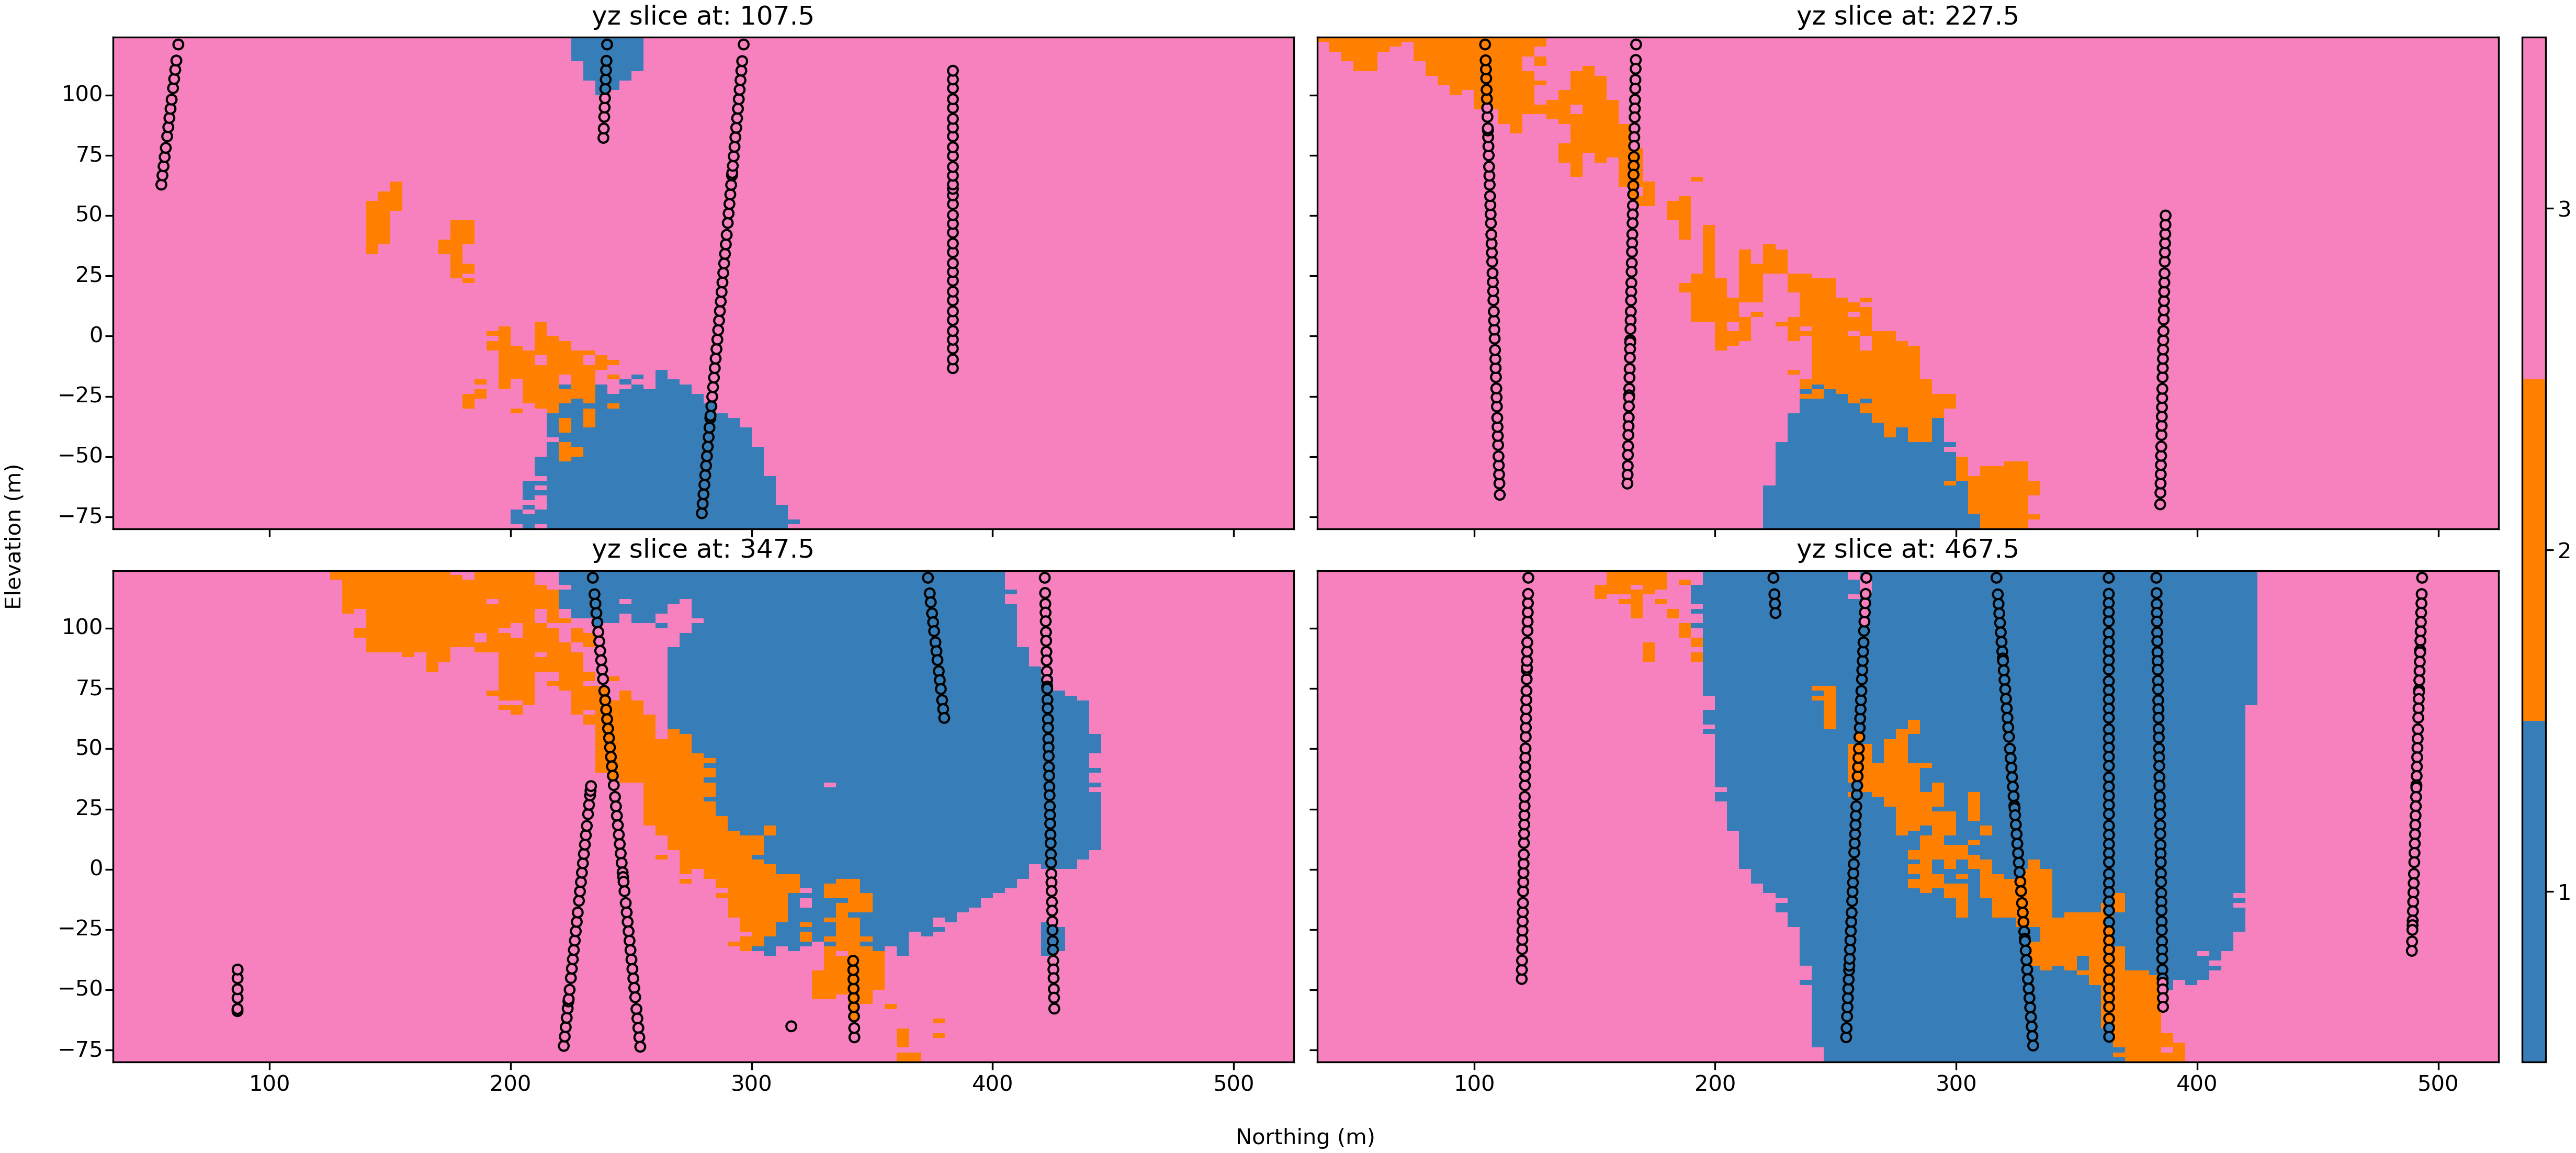
\includegraphics[width=0.8\textwidth]{capitulo_2/directsimreal1.png}\label{a}}\\
\end{center}
\begin{center}
\subfloat[][Realização 2]{\includegraphics[width=0.8\textwidth]{capitulo_2/directsimreal2.png}\label{b}}
\end{center}
\end{figure}

O método é baseado em múltiplas realizações do modelo geológico, então, seu produto final pode ser usado nas etapas posteriores do processo de avaliação. Entretanto, a metodologia tem muitos passos \cite{radtke_dissertacao}

\begin{enumerate}
\item Cálculo das distâncias assinaladas para todas as amostras e categorias;
\item Variografia das distâncias no espaço original para todas as categorias;
\item Interpolação das distancias; 
\item criação do modelo com base na menor distância interpolada;
\item Criação da zona de incerteza;
\item Transformação Gaussiana das distâncias;
\item Variografia das distâncias no espaço gaussiano para todas as categorias;
\item Geração de múltiplos modelos baseados na menor distância simulada;
\item Validação e pós processamento das realizações.
\end{enumerate}

Além disso, a simulação é muito sensível aos parâmetros, o que muitas vezes, gera modelos com muito ruído, que não são geologicamente realistas, e não honram as amostras, como os da \autoref{dif_real}. O resultado final não justifica o número excessivo de passos e parâmetros. O coeficiente U não controla a magnitude da incerteza, apenas diminui o tempo das simulações, o magnitude da incerteza é controlada pelo parâmetros da simulação.

\subsection{Simulação multi ponto}

\citeonline{silvaenhancedgeomodeling} propôs uma metodologia que integra modelagem geológica implícita com funções distâncias assinaladas e simulação geostatística multi ponto. A geostatística multi ponto utiliza imagens de treinamento para extrair e reproduzir estruturas geológicas complexas. Geralemnte, imagens de trinamento são baseadas em modelos conceituais do fenômeno geoógico. Em seu trabalho, \citeonline{silvaenhancedgeomodeling} cria imagens de trinamento a partir de modelos geológicos implícitos determinísticos criados com funções distância assinaladas e modelos estocásticos criados por simulação sequencial dos indicadores. No trabalho é introduzida uma metodologia  para integrar múltiplas imagens de treinamento, uma metodologia para calibrar a contribuição de cada imagem de treinamento e uma medida de entropia multi ponto ao longo dos furos de sondagem.

\citeonline{silvaenhancedgeomodeling} concluiu que imagens de treinamento geradas a partir das amostras produzem modelos geológicos estocásticos por MPS melhores. A \autoref{snesim_real} mostra duas realizações do modelo geológico criado a partir da aplicação do algoritmo \verb|snesim| usando a \autoref{multi_cat_rbf} como imagem de treinamento. 

\begin{figure}[t]
\caption{Diferentes realizações do modelo geológico.} 
\label{snesim_real}
\begin{center}
\subfloat[][Realização 1]{\includegraphics[width=0.8\textwidth]{capitulo_2/snesim_real1.png}\label{a}}\\
\end{center}
\begin{center}
\subfloat[][Realização 2]{\includegraphics[width=0.8\textwidth]{capitulo_2/snesim_real2.png}\label{b}}
\end{center}
\end{figure}

Os modelos mostram realismo geológico, não apresentam ruido excessivo. Além disso, o método é rápido e não depende de um grande número de parâmetros. Em contrapartida, não é possível controlar a magnitude da incerteza. 

\subsection{\textit{Boundary simulation}}\label{boundsim}

A metodologia proposta por \citeonline{wilde_sim_bound_reals} consiste em gerar realizações das fronteiras geológicas comparando distâncias modificadas interpoladas com simulações não condicionais. 

O primeiro passo é calibrar os parâmetros de incerteza, \citeonline{munroe_c_full_calibration} propuseram a calibração completa dos parâmetros C e $\beta$, onde C controla a largura da bande de incerteza e $\beta$ controla o viés. Os parâmetros devem ser otimizados para que a incerteza apropriada seja avaliada. Otimizar esses parâmetros é uma operação computacionalmente cara que requer múltiplos modelos de referência e duas funções objetivo \cite{wilde2012kriging}.

\citeonline{kaperov_review_boundary} propuseram uma metodologia de calibração para o parâmetro C simplificada, de modo empírico. considerando a malha amostral e a experiência e conhecimento do geomodelador.

\citeonline{wilde_new_way} propuseram uma outra metodologia de calibração, nessa metodologia apenas o parâmetro C é calibrado usando apenas as amostras disponíveis. Um subconjunto das amostras é removido antes do cálculo das distâncias assinaladas. Isso cria dois diferentes bancos dados: o banco de dados das distâncias assinaladas e o banco de dados \textit{jackknife}. O banco de dados das distâncias assinaladas é usado para condicionar a estimativa das distâncias nos locais do banco de dados \textit{jackknife}. Algumas amostras do banco de dados \textit{jackknife} que foram codificadas como fora do domínio terão distâncias estimadas negativas (dentro do domínio) e vice-versa. O parâmetro C é ajustado até que uma proporção pré definida de classificação errônea seja atingida.

A \autoref{c_param_1} mostra a calibração do parâmetro C para a categoria 1 do banco de dados. 25\% das amostras foram removidas de forma aleatória 50 vezes, gerando 50 bancos de dados de distância e 50 bancos de dados \textit{jackknife}, as distâncias foram estimados nos locais das amostras \textit{jackknife} e a taxa de classificação errônea foi registrada no eixo y. o parâmetro C foi incrementado, e somado ou subtraídos das distâncias de acordo com a \autoref{C_dist}, o processo é repetido enquanto C varia de 0 até 250m. Quanto maior for o valor de C, menor o índice de classificação errônea.

\begin{figure}[!ht]
	\caption{\label{c_param_1}Calibração do parâmetro C para a categoria 1.}
	\begin{center}
		\includegraphics[width=0.6\textwidth]{capitulo_2/uncert_1.png}
	\end{center}
	%\legend{Fonte: \citeonline{rolo_dissertacao}}
\end{figure}

\begin{equation}
	d_k(u_\alpha)=\begin{cases}
	-\parallel u_\alpha-u_\beta\parallel - C,\:\textrm{se $u_\alpha$ pertence ao domínio}\\
	+\parallel u_\alpha-u_\beta\parallel + C,\:\textrm{se $u_\alpha$ não pertence ao domínio}\end{cases}
    \label{C_dist}
\end{equation}

O valor do parâmetro C deve ser determinado a partir da calibração (\autoref{c_param_1}). \citeonline{manchuck_deutsch_Geometric} sugerem 2,5\% de classificação errônea em nível aceitável para depósitos tabulares, uma outra forma de escolha é o método do cotovelo, o valor tomado deve ser o ponto de inflexão da curva. Para a categoria 1 foi tomado o valor de C igual a 130 que corresponde a um índice de classificação errônea de 2\%. As distâncias modificadas pelo parâmetro C a partir da \autoref{C_dist} devem ser interpoladas para todos os nós do grid, e a truncagem entre -C e C define a zona de incerteza.

Valores para a função distância são então simulados uniformemente entre -C e C. Caso o valor interpolado seja menor que o valor simulado para a função distância, o local é considerado pertencente ao domínio, caso o valor seja maior, o local é considerado externo ao domínio. Nos locais onde a interpolação apresenta o mesmo valor da simulação são estabelecidos os contatos dos domínios como esquematizado na \autoref{class}.

\begin{figure}[!ht]
	\caption{\label{class}Classificação dos locais comparando valores estimados e simulados.}
	\begin{center}
		\includegraphics[width=0.8\textwidth]{capitulo_2/classificacao.png}
	\end{center}
	\legend{Fonte: Modificado de \citeonline{wilde_sim_bound_reals}}
\end{figure}

Para que a simulação seja realizada de forma uniforme entre –C e +C, o desvio padrão $y`(u)$, deve ser simulado e transformado pela relação:

\begin{equation}
    df'(u)=2*C*G^-1(y'(u))-C
\end{equation}

Onde: $df'(u)$ é o valor da função distância simulada, $y'(u)$ o valor normal padrão da simulação não condicional, e $G^-1$ representa a determinação do valor da distribuição acumulada padrão normal correspondente a $y'(u)$. Para garantir que os valores pertençam a região estabelecida. os valores são multiplicados por 2C e subtraídos de C.

O variograma utilizado na simulação não condicional pode ser o mesmo das distâncias assinaladas. O alcance do variograma determina a natureza do contato entre os domínios, menores alcances geram contatos mais rugosos enquanto maiores alcances, contatos suaves.

A \autoref{cat1_bound_sim} mostra as distâncias interpoladas e simuladas na zona de incerteza para a a categoria 1, definida entre -120m e 120m e os blocos classificados em pertencentes à categoria ou não. As probabilidades de cada bloco pertencer à categoria 1 pode ser calculada tomando a média dos blocos classificados com 1 ou 0 em todas as realizações.

\begin{figure} 
    \caption{Interpolação, simulação e classificação na zona de incerteza.} \label{cat1_bound_sim}
     \centering
     \subfloat[][Distâncias interpoladas]{\includegraphics[width=.3\textwidth]{capitulo_2/interpolated.jpeg}\label{<figure1>}}
     \subfloat[][Distâncias simuladas]{\includegraphics[width=.3\textwidth]{capitulo_2/simulated.jpeg}\label{<figure2>}}
     \subfloat[][Classificação]{\includegraphics[width=.3\textwidth]{capitulo_2/classification.jpeg}\label{<figure2>}}
\end{figure}

A \autoref{cpar_real} mostra seções em XY e YZ de uma das realizações para a categoria 1.

\begin{figure}[t]
\caption{Seções verticais de uma realização para a categoria 1.} 
\label{cpar_real}
\begin{center}
\subfloat[][Seção em XY]{\includegraphics[width=0.8\textwidth]{capitulo_2/cpar1.png}\label{a}}\\
\end{center}
\begin{center}
\subfloat[][Seção em YZ]{\includegraphics[width=0.8\textwidth]{capitulo_2/cparyz.png}\label{b}}
\end{center}
\end{figure}

O método é rápido já que é baseado em simulações não condicionais, gera modelos realistas sem ruído e com fronteiras contínuas. Tanto a magnitude da incerteza quanto a natureza da fronteira podem ser controlados. Entretanto, o método funciona apenas para uma categoria por vez e mesmo que simplificações tenham sido desenvolvidas, a calibração do parâmetro de incerteza ainda pode ser laboriosa e subjetiva.

\citeonline{amarante_incerteza_associada} propuseram uma adaptação  do método para múltiplas categorias simultâneas, uma série de regras hierárquicas baseadas na cronologia dos eventos geológicos devem ser definidas, a \autoref{hier_ex} mostra um esquema do método, evidenciando as regras de hierarquização e realizações dos grupos formados. Embora seja uma alternativa para ambientes multi categóricos, a definição das regras de hierarquização dependem de conhecimento geológico além das amostras, e muitas vezes indisponível.

\begin{figure}[!ht]
	\caption{\label{hier_ex}Esquema do método mostrando as regras de hierarquização e diferentes realizações dos grupos formados.}
	\begin{center}
		\includegraphics[width=0.9\textwidth]{capitulo_2/hier_example.png}
	\end{center}
	\legend{Fonte: \citeonline{amarante_incerteza_associada}}
\end{figure}

\subsection{Sumário dos métodos de avaliação de incerteza}

A \autoref{sumario} mostra um sumário dos métodos de incerteza que avalia: a simplicidade, o método deve, preferencialmente, ser simples e direto, não deve envolver um número excessivo de passos ou matemática complicada. A velocidade, o método deve ser de rápida execução. A capacidade de trabalhar em ambientes multi categóricos de forma direta, sem a necessidade de abordagens hierárquicas subjetivas. O realismo geológico, as formas geradas devem ser suaves e não apresentar ruído excessivo. O controle da incerteza, a incerteza deve ser controlada a partir de bandas de incerteza ou a partir dos parâmetros de simulação. Finalmente, a natureza do contato, ruidoso ou suave, deve ser controlada.

% Table generated by Excel2LaTeX from sheet 'Planilha1'
\begin{table}[htbp]
  \centering
  \resizebox{\textwidth}{!}{%
    \begin{tabular}{lcccccc}
    Método & \multicolumn{1}{l}{Simplicidade} & \multicolumn{1}{l}{Velocidade} & \multicolumn{1}{l}{Multi categórico} & \multicolumn{1}{l}{Realismo geológico} & \multicolumn{1}{l}{Controle da incerteza} & \multicolumn{1}{l}{Controle do tipo de contato} \\
    \midrule
    Heurístico & simples & rápido & sim   & não   & sim   & não \\
    Boundsim & simples & rápido & não   & sim   & não   & não \\
    Simulação direta & complexo & demorado & sim   & não   & sim   & não \\
    MPS   & simples & rápido & sim   & sim   & não   & não \\
    Boundary simulation & simples  & rápido & não   & sim   & sim   & sim \\
    \bottomrule
    \end{tabular}%
    }
  \caption{Sumário dos métodos de avaliação de incerteza de modelos geológicos.}\label{sumario}%
\end{table}%




